\documentclass{report}

\usepackage[utf8]{inputenc}
\usepackage{graphicx}
\usepackage[greek]{babel}

\usepackage{alphabeta}

\linespread{1.5}
\usepackage{minted}
\usemintedstyle{perldoc}
\oddsidemargin = 0pt
\marginparsep = 30pt
\textwidth = 450pt
\documentclass[14pt]
\usepackage{tgadventor}
\usepackage[LGR, T1]{fontenc}

\graphicspath{ {/Home/Pictures} }

\begin{document}

\vspace{5mm}

\begin{center}

\includegraphics{hualogo}
\end{center}

\vspace{5mm}

\begin{center}
ΧΑΡΟΚΟΠΕΙΟ ΠΑΝΕΠΙΣΤΗΜΙΟ ΑΘΗΝΩΝ
\end{center}

\vspace{5mm}

\begin{center}
ΣΧΟΛΗ ΨΗΦΙΑΚΗΣ ΤΕΧΝΟΛΟΓΙΑΣ
\end{center}
\begin{center}
ΤΜΗΜΑ ΠΛΗΡΟΦΟΡΙΚΗΣ ΚΑΙ ΤΗΛΕΜΑΤΙΚΗΣ
\end{center}

\vspace{10mm}

\begin{center}
ΠΤΥΧΙΑΚΗ ΕΡΓΑΣΙΑ
\end{center}

\begin{center}
Υλοποίηση του αλγορίθμου συστάσεων
\textlatin{SVD} στην πλατφόρμα \textlatin{Spark}
\end{center}

\vspace{5mm}

\begin{center}
Αλέξανδρος Ιωαννίδης
\end{center}

\vspace{5mm}

\begin{center}
Επιβλέποντες: 
\end{center}


\begin{center}
Ηρακλής Βαρλάμης, Επίκουρος Καθηγητής \end{center}


\begin{center}
Δημήτριος Μιχαήλ, Επίκουρος Kαθηγητής
\end{center}


\begin{center}
Κωνσταντίνος Τσερπές, Λέκτορας
\end{center}

\vspace{25mm}

\begin{center}
ΑΘΗΝΑ
\end{center}

\vspace{5mm}

\begin{center}
ΙΟΥΝΙΟΣ 2016
\end{center}
%-------------------------------------------------------------------------------------
\newpage

\begin{center}
ΠΤΥΧΙΑΚΗ ΕΡΓΑΣΙΑ         
\end{center}

\vspace{5mm}

\begin{center}
ΕΞΑΤΟΜΙΚΕΥΜΕΝΗ ΠΑΡΟΧΗ ΣΥΣΤΑΣΕΩΝ ΜΕ ΒΑΣΗ ΤΟ ΠΕΡΙΕΧΟΜΕΝΟ ΚΑΙ ΤΙΣ ΠΡΟΤΙΜΗΣΕΙΣ
\end{center}

\vspace{10mm}

\begin{center}
Αλέξανδρος Ιωαννίδης
\end{center}

\begin{center}
Α.Μ.: 21208
\end{center}

\vspace{10mm}

\begin{center}

\includegraphics{sparklogotrademark}
\end{center}

\vspace{5mm}

\begin{center}

\includegraphics{mllogo}
\end{center}

\vspace{20mm}

\begin{center}
Επιβλέποντες:  Ηρακλής Βαρλάμης, Επίκουρος Καθηγητής 
\end{center}
%-------------------------------------------------------------------------------------
\newpage



\begin{center}
Στον πατέρα μου Θεόφιλο, \\
στην μητέρα μου Μόνικα, \\
στην αδελφή μου Ελένη, \\
και στους φίλους μου Μανόλη και Σωκράτη
\end{center}

\newpage
\begin{center}
\huge{Περιεχόμενα}
\end{center}


\vspace{16mm}


\text{ ΠΡΟΛΟΓΟΣ ............................................................................................................... 7}
    \vspace{10mm}


\begin{list}
\textbf{1. ΕΙΣΑΓΩΓΗ.............................................................................................................. 8 }
   \vspace{2mm} 
    \item{1.1 Πεδίο διατριβής ................................................................................................... 8 }
    \item{1.2 Σκοπός ............................................................................................................... 8 }
    \item{1.3 Σύνοψη αποτελεσμάτων....................................................................................... 9}
    \vspace{5mm}
\end{list}


\begin{list}
\textbf{2. ΕΠΙΣΤΗΜΟΝΙΚΟ ΥΠΟΒΑΘΡΟ............................................................................. 11}
   \vspace{2mm} 
    \item{2.1 Βασικές έννοιες και βασικές βιβλιογραφικές αναφορές.......................................... 11}
    \item{2.2 Σχετικές επιστημονικές εργασίες ......................................................................... 12}
    \item{2.3 Περιγραφή συστημάτων που χρησιμοποιήθηκαν στη διατριβή................................ 13}
    \vspace{5mm}
\end{list}

\begin{list}
\textbf{3. ΑΝΑΛΥΣΗ ΤΗΣ ΠΡΟΣΕΓΓΙΣΗΣ ......................................................................... 17}
   \vspace{2mm} 
    \item{3.1 Θεωρητική διατύπωση του προβλήματος............................................................... 17}
    \item{3.2 Απαιτούμενη λειτουργικότητα .............................................................................. 17}
    \vspace{5mm}
\end{list}

\begin{list}
\textbf{4. ΣΧΕΔΙΑΣΗ ............................................................................................................ 19}
   \vspace{2mm} 
    \item{4.1 Αρχιτεκτονικό διάγραμμα .................................................................................... 19}
    \item{4.2 Περιγραφή υποσυστημάτων - λειτουργιών............................................................. 20}
    \vspace{5mm}
\end{list}

\begin{list}
\textbf{5. ΥΛΟΠΟΙΗΣΗ .............................................................................................................. 28}
   \vspace{2mm} 
    \item{5.1 Λεπτομέρειες υλοποίησης  ......................................................................................... 28}
    \item{5.2 Οθόνες εφαρμογής ................................................................................................... 40}
    \vspace{5mm}
\end{list}

\begin{list}
\textbf{6. ΑΠΟΤΕΛΕΣΜΑΤΑ - ΑΞΙΟΛΟΓΗΣΗ........................................................................... 44}
   \vspace{2mm} 
    \item{6.1 Μετρικές αξιολόγησης και συγκριτική αξιολόγηση...................................................... 44}
    \item{6.2 Αποτελέσματα............................................................................................................ 46}
    \vspace{5mm}
\end{list}

\begin{list}
\textbf{7. ΣΥΜΠΕΡΑΣΜΑΤΑ ...................................................................................................... 48}
   \vspace{2mm} 
    \item{7.1  Σύνοψη προτεινόμενης προσέγγισης με καινοτόμα στοιχεία και θετικά αποτελέσματα. 48}
    \item{7.2 Δυσκολίες που παρουσιάστηκαν................................................................................. 48}
    \item{7.3 Πιθανός χώρος για βελτιώσεις.................................................................................... 64}
    \item{7.4 Μελλοντικές επεκτάσεις.............................................................................................. 65}
    \vspace{5mm}
\end{list}

\begin{list}
\textbf{Βιβλιογραφία ....................................................................................................................... 67}
\item{}
\end{list}

\begin{list}
\textbf{Παραρτήματα ....................................................................................................................... 71}
\item{Πρόγραμμα \textlatin{C++} με \textlatin{MovieLens datasets} ........................................................................ 71}
\item{Πρόγραμμα \textlatin{Java} με \textlatin{MovieLens datasets} ......................................................................... 83}.
\item{Πρόγραμμα \textlatin{Java} στο \textlatin{Apache Spark} με \textlatin{MovieLens datasets} ............................................ 95}
\end{list}
%-------------------------------------------------------------------------------------
\newpage

\begin{center}
\huge{ΚΑΤΑΛΟΓΟΣ ΣΧΗΜΑΤΩΝ}
\end{center}
\\
Σχήμα 1: Σχήμα αρχιτεκτονικού διαγράμματος για σειριακό κώδικα ............................................. 19
\\
Σχήμα 2: Σχήμα αρχιτεκτονικού διαγράμματος για παράλληλο κώδικα........................................... 20

 \vspace{25mm}
 
\begin{center}
\huge{ΚΑΤΑΛΟΓΟΣ ΕΙΚΟΝΩΝ}
\end{center}
\\
Εικόνα 1: Εικόνα από την εκτέλεση του σειριακού κώδικα σε \textlatin{C++ MovieLens} .........................  41
\\
Εικόνα 2: Εικόνα από την εκτέλεση του σειριακού κώδικα σε \textlatin{Java MovieLens} .......................... 42
\\
Εικόνα 3: Εικόνα από την εκτέλεση του παράλληλου κώδικα σε \textlatin{Java} στο \textlatin{Spark} ....................... 42
%-------------------------------------------------------------------------------------
\newpage

\begin{center}
\LARGE{ΠΡΟΛΟΓΟΣ}
\end{center}

\vspace{10mm}

\par{ Η παρούσα πτυχιακή εργασία με τίτλο «Εξατομικευμένη παροχή συστάσεων με βάση το περιεχόμενο και τις προτιμήσεις» διενεργήθηκε στο πλαίσιο της υποχρεωτικής εκπόνησης πτυχιακής εργασίας στο κτίριο που στεγάζεται το τμήμα Πληροφορικής και Τηλεματικής του Χαροκοπείου Πανεπιστημίου Αθηνών.
}

\par { Η διεκπεραίωση της πτυχιακής εργασίας  επιτεύχθει με την αναλυτική καθοδήγηση και στενή παρακολούθηση του Επίκουρου Καθηγητή Βαρλάμη Ηρακλή και τον οποίο θα ήθελα να ευχαριστήσω για όλες τις άμεσες και επεξηγηματικές απαντήσεις του σε όλες τις απορίες μου.
}

%-------------------------------------------------------------------------------------
\newpage

%\fancyhead[L]{Εξατομικευμένη παροχή συστάσεων με βάση το περιεχόμενο και τις προτιμήσεις}

\begin{center}

\LARGE{1. ΕΙΣΑΓΩΓΗ}

\end{center}

\vspace{2mm} 

\textbf{\large{1.1 Πεδίο διατριβής}}

\vspace{2mm}

Το θέμα της διατριβής, αφορά την επέκταση ενός συστήματος στηριζόμενο σε λογισμικό, το οποίο προτρέπει χρήστες μιας ιστοσελίδας  εικονικής κοινότητας, με συμβουλευτικές προτάσεις για τη παρακολούθηση νέων ταινιών προσαρμοσμένες στις ανάγκες του κάθε χρήστη ξεχωριστά, όπως το γνωστό \textlatin{MovieLens}.
\vspace{1mm}

\\
Η δημιουργία των προτάσεων, προκύπτει από την συσσώρευση πληροφοριών, από το περιεχόμενο κάθε χρήστη και την ιστορική καταγραφή των προτιμήσεών του, σύμφωνα με τη συμμετοχή του σε προηγούμενες ψηφοφορίες στις οποίες έχει κληθεί να βαθμολογήσει ταινίες. Το σύστημα αναπτύχθηκε με τη μέθοδο συνεργατικού φιλτραρίσματος \textlatin{Collaborative Filtering (CF)} με την στενότερη έννοια, δηλαδή δημιουργώντας αυτόματες προβλέψεις για τους χρήστες. Μια από τις μεθόδους που υλοποιείται το \textlatin{(CF)} και στην οποία βασίζεται το λογισμικό που έχει αναπτυχθεί, είναι η υβριδική μέθοδος που συνδυάζει δύο τεχνικές πρώτον με βάση το περιεχόμενο του χρήστη \textlatin{(content based)} και δεύτερον το \textlatin{(item based)} το οποίο είναι το ιστορικό των προτιμήσεων κάθε χρήστη.

Το ήδη υπάρχον λογισμικό που πρόκειται να επεκταθεί σε άλλη γλώσσα προγραμματισμού από μέρους μου, παρουσιάζει έναν αλγόριθμο που υλοποιεί την προηγούμενη υβριδική μέθοδο. Ο
αλγόριθμος αυτός είναι ο \textlatin{Singular Value Decomposition (SVD)}.

Οι συστάσεις που γίνονται από το σύστημα στο χρήστη, προκύπτουν με βάση την επεξεργασία των αποθηκευμένων στοιχείων που αφορούν τον κάθε χρήστη και από τον αλγόριθμο \textlatin{(SVD)} ο οποίος υπολογίζει και εξάγει με τη παραγοντοποίηση ενός πολύπλοκου πίνακα ο οποίος περιέχει στατιστικά στοιχεία με βάση τα οποία γίνονται οι προβλέψεις για τη πιθανή μελλοντική συμπεριφορά ενός χρήστη. 

\vspace{20mm} 


\textbf{\large{1.2 Σκοπός}}

\vspace{2mm}

Στόχος της παρούσας πτυχιακής εργασίας, είναι η επέκταση υπάρχουσας εφαρμογής με την συμβολή της βιβλιοθήκης \textlatin{Lenskit}. Σε αυτό το σκοπό συμπεριλαμβάνονται τα ακόλουθα στάδια, πρώτα η παραμετροποίηση του αρχικού σειριακού κώδικα δοσμένου σε \textlatin{C++} έτσι ώστε να δέχεται ως είσοδο τα \textlatin{dataset} του \textlatin{MovieLens}, έπειτα μετατροπή του ήδη υπάρχοντος προγράμματος σειριακής ακολουθίας, κατασκευασμένου σε γλώσσα προγραμματισμού \textlatin{C}++ σε σειριακό πρόγραμμα, με χρήση της γλώσσας προγραμματισμού \textlatin{Java}, και έπειτα η μετατροπή του σειριακού κώδικα ανεπτυγμένου σε \textlatin{Java} σε παράλληλο πρόγραμμα χρησιμοποιώντας την πλατφόρμα ανάπτυξης
\textlatin{Apache Spark} η οποία αποτελεί μια γρήγορη μηχανή επεξεργασίας δεδομένων μεγάλης κλίμακας και της γλώσσας προγραμματισμού \textlatin{Java}.
\vspace{1mm}

\\  Τελικά, γίνεται η χρονική καταγραφή της εκτέλεσης του σειριακού προγράμματος αναπτυγμένου σε \textlatin{Java} και του αντίστοιχου παράλληλου προγράμματος επίσης σε \textlatin{Java} έτσι ώστε να διαπιστωθεί αν παράγονται παρόμοια αποτελέσματα και να γίνει αντιπαραβολή των διαφορετικών χρόνων εκτέλεσης των προγραμμάτων και να παρατηρηθεί αν έχει επιτευχθεί κάποια βελτιστοποίηση με τη παραλληλοποίηση ή όχι, και συμπερασματικά αν υπάρχουν περιθώρια περαιτέρω βελτίωσης του προγράμματος.

\vspace{25mm}
\\
\textbf{\large{1.3 Σύνοψη αποτελεσμάτων}}
\vspace{2mm}
\\
Συνοπτικά, τα αποτελέσματα που προέκυψαν ήταν αρχικά από την παραμετροποιήση του αρχικού κώδικα σε \textlatin{C++}, δηλαδή η εξαγωγή των αποτελέσμάτων για το \textlatin{dataset} του \textlatin{MovieLens} των 100000 βαθμολογιών, έπειτα με την εκτέλεση του σειριακού κώδικα που μετατράπηκε σε \textlatin{Java} διαπιστώθηκε αξιοσημείωτη βελτίωση στον συνολικό χρόνο υλοποίησης καθώς επίσης και στους χρόνους εκτέλεσης των επιμέρους μεθόδων συγκριτικά με τον αρχικό κώδικα σε \textlatin{C++}. Η διάρκεια για την κατασκευή του \textlatin{engine}, του \textlatin{load history} και του \textlatin{processing test}  είναι 0 \textlatin{seconds}, άρα συνολικά 6 \textlatin{seconds}, χρησιμοποιώντας ως \textlatin{training file} το \textlatin{u.data} το οποίο αποτελεί ολόκληρο το \textlatin{data set} αυτό των 100.000 βαθμολογιών όπου και οι χρήστες και οι ταινίες είναι απαριθμημένα συνεκτικά από το 1. Ως  \textlatin{testing file}  χρησιμοποιήθηκε το \textlatin{u1.test} το οποίο αποτελείται από 2 κομμάτια, το πρώτο κομμάτι αποτελεί το 80\% του συνόλου και είναι από το \textlatin{u data} και το δεύτερο κομμάτι αποτελεί το 20\% του συνόλου και είναι από το \textlatin{test data}. Τέλος χρησιμοποιήθηκε το \textlatin{u1.predictions} αντίστοιχα για να γραφτούν τα παραγόμενα αποτελέσματα με μέση εκτίμηση λάθους να είναι 0,679812.

Στην συνέχεια το παράλληλο πρόγραμμα υλοποιημένο σε \textlatin{Java} στο \textlatin{Spark} επιτυγχάνει την παραλληλοποιήση όλων των \textlatin{function} εκτός της \textlatin{CalcFeatures} η οποία εκτελείται ακολουθιακά όπως προηγουμένως. Συγκεκριμένα ο χρόνος υλοποιήσης του \textlatin{engine construction} διαρκεί 5 \textlatin{seconds}, της \textlatin{LoadHistory} 3 \textlatin{seconds} και η \textlatin{ProcessTest} 1 \textlatin{second}, ενώ η εκτέλεση για τη \textlatin{CalcFeatures} που εκτελείται σειριακά είναι 18 \textlatin{seconds}. Συνεπώς ο συνολικός χρόνος εκτέλεσης του παράλληλου προγράμματος είναι 27 \textlatin{seconds} χρησιμοποιώντας το \textlatin{MoovieLens Dataset} ίδιου μεγέθους με αυτό που χρησιμοποιήθηκε στα άλλα 2 προγράμματα δηλαδή αυτό των 100.000 βαθμολογιών.   
 
Η  υλοποιήση της \textlatin{function CalcFeatures} δυστυχώς παρέμεινε σειριακή λόγω των περιορισμών παραλληλοποιήσης που έχει ο αρχικός αλγόριθμος σε αυτό το κομμάτι του.  
    
 Η κυρίως εργασία του αλγορίθμου γίνεται με τη μέθοδο \textlatin{CalcFeatures} που σκοπό έχει τον υπολογισμό των τιμών στους 2 πίνακες \textlatin{CustomerFeatures} και \textlatin{MovieFeatures}. Οι τιμές στα κελιά των πινάκων αυτών ενημερώνονται κατά κύματα \textlatin{(epochs) }μέχρι να επιτευχθεί κάποιο αποδεκτό συνολικό σφάλμα. Η εργασία αυτή αποτελείται από 3 ένθετους βρόχους, με κατ' ελάχιστο εκτελέσεις των εντολών του εσωτερικού βρόγχου να είναι [10^5 * 120 * 64 = 768000000]. 
 
  Οι εντολές αυτές είναι κυρίως οι 4 βασικές πράξεις αριθμητικής και ανάγνωση και εγγραφή σε 2 δισδιάστατους και έναν μονοδιάστατο πίνακα.
  
  Επιπρόσθετα όλοι οι πίνακες έχουν μετατραπεί σε κάποιο \textlatin{RDD<Type>}, οποιαδήποτε διάβασμα αλλά και τροποποίηση δεδομένων απαιτεί κάποιο \textlatin{transformation} ή \textlatin{action} πάνω στο \textlatin{RDD}. Για τα \textlatin{transformation} χρειάζεται να περιγραφεί η μετατροπή με \textlatin{lambda expression, anonymous class, inner class} ή \textlatin{static nested class}. Για να επιτευχθεί η επιθυμητή λειτουργικότητα \textlatin{R/W} σε πολλαπλά \textlatin{RDD} σε ένα ενιαίο βήμα, θα έπρεπε να μπορεί να γίνει κλήση \textlatin{RDD transformation/action} μέσα από την \textlatin{function} του \textlatin{anonymous class/lambda expression,} πράγμα που απαγορεύεται στο \textlatin{Spark}. 
 
 Στην ενότητα 7 με τα συμπεράσματα γίνεται μια αναλυτική περιγραφή με τα αναλυτικά συμπεράσματα, την αδυναμία παραλληλοποίησης ενός συγκεκριμένου τμήματος κώδικα και τις δυσκολίες που παρουσιάστηκαν κατά την διαδικασία εκπόνησης της παρούσας πτυχιακής εργασίας.
 

\newpage

\begin{center}
\LARGE{2. ΕΠΙΣΤΗΜΟΝΙΚΟ ΥΠΟΒΑΘΡΟ}
\end{center}

\vspace{5mm}

\textbf{\large{2.1 Βασικές έννοιες και βασικές βιβλιογραφικές αναφορές}}
\vspace{2mm}
\\
Σημαντικές έννοιες, που εμπεριέχονται στην υπάρχουσα εργασία, είναι αρχικά η έννοια του \textlatin{recommendation system} το οποίο αποτελεί μια υποκλάση ενός συστήματος φιλτραρίσματος πληροφοριών που έχει ως σκοπό την αναζήτηση της πρόβλεψης της βαθμολογίας ή της προτίμησης των χρηστών σε αντικείμενα. Δημοφιλής εφαρμογές στις οποίες χρησιμοποιούνται συνήθως είναι σε ταινίες όπως και στη περίπτωση της τρέχουσας εργασίας αλλά και σε τραγούδια.  

Επιπρόσθετα, η έννοια του \textlatin{Collaborative filtering} είναι μια τεχνική που χρησιμοποιείται από τη προαναφερθείσα έννοια \textlatin{recommendation system} και διακρίνεται σε 2 έννοιες την πιο στενή και την πιο γενική. Νεότερη καθώς επίσης και αυτή που εξετάζεται στην εργασία είναι η στενότερη έννοια στην οποία η διαδικασία του φιλτραρίσματος αφορά τις πληροφορίες των χρηστών ή ακόμα καλύτερα τη τάση που έχουν να συμπεριφέρονται οι χρήστες. Επιπλέον αυτή η τεχνική δημιουργεί αυτόματες προβλέψεις για τα ενδιαφέροντα των χρηστών συλλέγοντας πληροφορίες για τις προτιμήσεις ή τη συσχέστιση της συμπεριφοράς πολλών χρηστών ή και τα δύο μαζί ταυτόχρονα.

Πρόσθετα, σπουδαία κρίνεται η σημασία του αλγορίθμου \textlatin{singular value decomposition} ο οποίος υλοποιεί τη παραγοντοποίηση ενός σχήματος \textlatin{U}Σ\textlatin{V}*  όπου το \textlatin{U} αποτελεί έναν \textlatin{m x m} μοναδιαίο πίνακα, το \textlatin{Σ} αποτελεί έναν \textlatin{m x n} διαγώνιο πίνακα χωρίς αρνητικούς αριθμούς στη κύρια διαγώνιό του και το \textlatin{V}* αποτελεί τον συζυγή ενός \textlatin{n x n} μοναδιαίου πίνακα.
 
Επίσης, σημαντική είναι η έννοια του \textlatin{data set} που αποτελεί μια συλλογή  σχετικών και διακριτών στοιχείων από συσχετιζόμενα δεδομένα που είναι οργανωμένα σε κάποιο είδος δομής δεδομένων που μπορούν να προσπελαστούν ατομικά ή σε συνδυασμό ή διαχειρίζονται στο σύνολο σαν οντότητα.  Μια βάση δεδομένων μπορεί να θεωρηθεί ένα σύνολο δεδομένων, όπως και τα υποτμήματα των δεδομένων μέσα σε μια ΒΔ που συσχετίζονται με ένα συγκεκριμένο είδος πληροφοριών.
 
Από κάτω, παραθέτονται βιβλιογραφικές  αναφορές που ξεχωρίζουν για τη σημαντικότητά τους και τη συνεισφορά τους στη διεκπεραίωση της πτυχιακής εργασίας.

Από τη βιβλιογραφική αναφορά με τον αριθμό [4], χρησιμοποιήθηκε το δείγμα του πηγαίου κώδικα σε
γλώσσα προγραμματισμού \textlatin{C++} που υλοποιεί τον αλγόριθμο \textlatin{SVD}, ως σημείο αναφοράς για την παρούσα
εργασία. Ο προηγούμενος αυτός κώδικας, τροποποιήθηκε στην ίδια γλώσσα προγραμματισμού έτσι ώστε
να δέχεται ως είσοδο \textlatin{dataset} στη μορφή του \textlatin{MovieLens}, έπειτα μετατράπηκε σε πρόγραμμα \textlatin{Java} σειριακής
ακολουθίας και έπειτα επεκτάθηκε σε παράλληλο πρόγραμμα επίσης αναπτυγμένο σε \textlatin{Java}.
Η βιβλιογραφική αναφορά με τον αριθμό [5], προχωράει ένα βήμα μακρύτερα και επεξηγεί πιο αναλυτικά
τα κομμάτια που περιέχουν μαθηματικές πράξεις και σύμβολα για τον υπολογισμό του \textlatin{SVD} βασισμένο στο
πηγαίο κώδικα από τη πηγή [4].
Από τη πηγή [7], αξιοποιήθηκαν θεμελιώδεις γνώσεις για τη χρησιμότητα αλλά και για τη κατανόηση
της λειτουργίας του διαδικτυακού ιστότοπου \textlatin{Movie Lens} καθώς κατά την διαδικασία ανάπτυξης και ελέγχου
των αποτελεσμάτων των προγραμμάτων χρησιμοποιούνται τα \textlatin{data sets} του \textlatin{Movie Lens}.
Από τη πηγή [8], βρέθηκαν και χρησιμοποιήθηκαν τα \textlatin{data sets} του \textlatin{Movie Lens}. Κυρίως χρησιμοποι
ήθηκε το \textlatin{data set} με τις 100.000 βαθμολογίες.
Από τη πηγή [9], αντλήθηκαν πολλές πληροφορίες για τον τρόπο εγκατάστασης και χρήσης της πλαtφόρμας \textlatin{Apache Spark} σε εφαρμογές με \textlatin{Java} και σε περιβάλλον λειτουργικού συστήματος \textlatin{Linux}.


\vspace{5mm}

\textbf{\large{2.2  Σχετικές επιστημονικές εργασίες }}

\vspace{2mm}

Κατά τη διάρκεια εκπόνησης της πτυχιακής εργασίας μου, εντόπισα ορισμένες πτυχιακές εργασίες με συνα-
φές αντικείμενο με το δικό μου. Συγκεκριμένα παραθέτονται οι πηγές από [10] έως [13] τις οποίες θεώρησα
σημαντικότερες.
Από τη πηγή [10] στην οποία παρουσιάζεται μια γενική περιγραφή των \textlatin{recommendation system} και των
σύγχρονων μεθόδων που τα υλοποιούν και οι οποίες είναι το \textlatin{content-based}, \textlatin{collaborative} και το \textlatin{hybrid}.
Ειδική έμφαση δόθηκε στη παράγραφο 2.3.1, 2.3.2 και 2.3.3 όπου περιγράφεται η διαδικασία πρόσθεσης
content-based χαρακτηριστικών σε collaborative μοντέλα για τη δημιουργία hybrid μεθόδων.
Αναλυτικότερα, από τη πηγή [11] η οποία αποτελεί έρευνα της Microsoft τριών ατόμων, στην οποία
έκαναν μια αναλυτική σύγκριση διαφόρων μεθόδων για την υλοποίηση του \textlatin{(CF)} με 2 διαφορετικές μετρικές
13
αξιολόγησης, η πρώτη χαρακτηρίζεται από ακρίβεια σε ένα σύνολο από ατομικές προβλέψεις ως προς την
απόλυτη μεσαία τυπική απόκλιση, ενώ η δεύτερη μετρική υπολογίζει τη χρησιμότητα μιας βαθμολογημένης
λίστας προτεινόμενων αντικειμένων. Επίσης μέσα από την έμμεσα διεξοδική παρουσίαση των διαφορών με-
ταξύ memory-based αλγορίθμων και model-based μεθόδων κατανόησα καλύτερα τη λειτουργία της πρώτης
κατηγορίας που προβλέπει τις βαθμολογίες ενός ενεργού χρήστη βασιζόμενο σε μερικές πληροφορίες σχετι-
κά με τον χρήστη και ενός συνόλου από υπολογίσιμα βάρη από τη βάση δεδομένων των χρηστών συνολικά.
Ενώ στη δεύτερη περίπτωση, αντιλήφθηκα τον τρόπο που υπολογίζεται η αναμενόμενη τιμή μιας ψηφοφο-
ρίας για αντικείμενα που δεν έχουν παρακολουθηθεί ακόμα από έναν χρήστη, με βάση τα αποτελέσματα
προηγούμενων ψηφοφοριών στις οποίες έχει συμμετάσχει ο ίδιος.
Στη συνέχεια, η πηγή [12] που αποτελεί Διπλωματική εργασία άλλου ατόμου στην οποία συμπεριλαμ-
βάνεται η υλοποίηση του αλγορίθμου \textlatin{SVD} για τη μείωση των διαστάσεων ενός διανυσματικού χώρου ως
μέρους ενός ευρύτερου προβλήματος και αφαιρώντας τις μειονεκτικές επιπτώσεις της πολλαπλής σημασίας
ή συνωνυμίας όρων διατυπώνοντας τις σημαντικές σχέσεις μεταξύ των όρων, βοήθησε αρκετά στη διαμόρ-
φωση μιας πιο σφαιρικής άποψης για την χρησιμότητα του αλγορίθμου. Επιπλέον κατανόησα καλύτερα
τη λειτουργία του αλγορίθμου καθώς επίσης και το ευρύ φάσμα εφαρμογών που έχει ο συγκεκριμένος
αλγόριθμος.
Τελικά, από τη πηγή [13] έγινε σαφέστερη η λειτουργία του \textlatin{SVD}, καθώς επίσης παρουσιάζει τρόπους
προσέγγισης του αλγορίθμου από προγραμματιστική σκοπιά, πως θα μπορούσαν να αναπαρισταθούν οι
\textlatin{SVD} πίνακες και πως μπορούν να υπολογιστούν οι τιμές τους και επιπλέον παρουσίασε μια εναλλακτική
προσέγγιση του αλγορίθμου που με βοήθησε αρκετά.



\vspace{20mm} 

\textbf{\large{2.3 Περιγραφή συστημάτων που χρησιμοποιήθηκαν στη διατριβή}}
\vspace{2mm}
\\
Για την συγγραφή της εργασίας, χρησιμοποιήθηκε το ευέλικτο σύστημα στοιχειοθεσίας κειμένων \textlatin{LaTex}, το οποίο μου επέτρεψε να εστιάσω περισσότερο στη λογική δομή του κειμένου, δίνοντας πολλές δυνατότητες σε εμένα, αλλά ίσως το βασικότερό του πλεονέκτημα είναι η γρήγορη ενσωμάτωση  εικόνων, πινάκων, \textlatin{cross-references} και τμημάτων κώδικα όπως επίσης και η εύκολη επεξεργασία τους. Πιο συγκεκριμένα χρησιμοποιήθηκε το \textlatin{ShareLaTeX} το οποίο είναι ένας \textlatin{online} επεξεργαστής \textlatin{LaTeX} που επιτρέπει την απευθείας σύνδεση και μεταγλώττιση των έργων σε \textlatin{PDF format}. Επίσης επειδή είναι εφαρμογή που στηρίζεται σε διακομιστή είχα πρόσβαση στη συγγραφή της παρούσας πτυχιακής εργασίας συνεχώς, ανεξαρτήτως τοποθεσίας μέσω ενός προγράμματος περιήγησης.  

Για την υλοποιήση της εργασίας, χρησιμοποιήθηκε αρχικά η πλατφόρμα ανάπτυξης λογισμικού \textlatin{Visual Studio 13} σε \textlatin{Windows 7} για την παραμετροποιήση του αρχικού αλγορίθμου υλοποιημένου σε \textlatin{C++} που δίνεται από τον ιστότοπο \textlatin{http://www.timelydevelopment.com/demos/NetflixPrize.aspx} έτσι ώστε να μπορεί να δέχεται ως είσοδο τα \textlatin{dataset} του \textlatin{MovieLens}. Για την εκτέλεση του προγράμματος σε \textlatin{C++} χρησιμοποιήθηε το \textlatin{Visual Studio 13} της \textlatin{Microsoft} όπως προανέφερα, πρόσβαση στο εργαλείο αυτό είχα από από τον υπολογιστή στο χώρο εργασίας μου σε λειτουργικό σύστημα \textlatin{Windows 7} για την εκτέλεση του προγράμματος σε λογισμικό της \textlatin{Microsoft} μόνο  και όχι από τον προσωπικό υπολογιστή μου που έχει σαν βασικό λειτουργικό σύστημα μόνο \textlatin{Ubuntu} 14.04. Τα χαρακτηριστικά του υπολογιστή εργασίας είναι επεξεργαστής \textlatin{Intel(R) Core(TM) i3 CPU 550, 3.20GHz, RAM 4,00 GB , 32-bit} αρχιτεκτονική συστήματος.

Με αυτόν τον τρόπο θα εξαχθούν αποτελέσματα από το \textlatin{predictions file} έτσι ώστε να χρησιμοποιηθούν στην συνέχεια για επαλήθευση των αποτελεσμάτων που θα προκύψουν από το σειριακό και παράλληλο πρόγραμμα μετέπειτα. Ύστερα αξιοποιήθηκε το \textlatin{Netbeans IDE} 8.1 για την μετατροπή του σειριακού κώδικα από \textlatin{C}++ σε σειριακό κώδικα σε \textlatin{Java}, σε υπολογιστή με βασικό λειτουργικό σύστημα \textlatin{Ubuntu} 14.04 και με τα εξής χαρακτηριστικά: επεξεργαστής \textlatin{Intel Core i7-4700MQ CPU 2.40 GHz x 8}, 24 \textlatin{GB RAM } και αρχιτεκτονική συστήματος 64-\textlatin{bit}. Έπειτα χρησιμοποιήθηκε η πλατφόρμα \textlatin{Apache Spark} σε συνδυασμό με τη πλατφόρμα ανάπτυξης λογισμικού \textlatin{IntelliJ IDEA} 15 επίσης σε λειτουργικό σύστημα \textlatin{Ubuntu} 14.04 για την ανάπτυξη της εφαρμογής παράλληλα. Η έκδοση του \textlatin{Apache Spark} 1.6.1 που χρησιμοποιήθηκε είναι η \textlatin{Pre-built} για το  \textlatin{Hadoop} 2.6 και μετά. Επίσης κατά τη διαδικασία εγκατάστασης του \textlatin{IntelliJ IDEA} έγινε και εγκατάσταση του \textlatin{SBT Plugin} το οποίο εργαλείο δίνει τη δυνατότητα παράλληλης εκτέλεσης εργασιών και συμπεριλαμβάνει την παράλληλη εκτέλεση δοκιμών.

Επίσης, για το σχεδιασμό και την υλοποιήση των διαγραμμάτων που θα ακολουθήσουν στη συνέχεια, χρησιμοποιήθηκε το λογισμικό \textlatin{Gliffy} το οποίο είναι \textlatin{SaaS} προσβάσιμο από παντού μέσω ενός προγράμματος περιήγησης και χρησιμοποιείτε κυρίως για τη δημιουργία \textlatin{UML} διαγραμμαάτων και \textlatin{flowcharts} καθώς επίσης το πρόγραμμα \textlatin{Dia} το οποίο είναι είναι ένα γενικού σκοπού λογισμικό για σχεδίαση διαγραμματών..  

Στη συνέχεια, για τη ανάπτυξη της παράλληλης υλοποίησης χρησιμοποίησα το \textlatin{Virtualbox} για τη δημιουργία δύο \textlatin{client} μηχανημάτων, και τα 2 έχουν λειτουργικό σύστημα \textlatin{Ubuntu} 14.04 όπως επίσης και ο \textlatin{server} που είναι το φυσικό μηχάνημα μου. Έτσι δημιούργησα ένα \textlatin{network-mounted shared file system}.

 Στον \textlatin{host-server} μηχάνημα μου τροποποιήσα το αρχείo \textlatin{/etc/exports} με διακιώματα \textlatin{root} και πρόσθεσα αυτή την εντολή \textlatin{/nfs} * \textlatin{(rw,sync,no\_root\_squash,no\_subtree\_check)} έτσι ώστε οτιδήποτε προστεθεί κάτω από το \textlatin{directory}  του διακομιστή \textlatin{/nfs} να είναι προσβάσιμο σε όλους τους πελάτες χωρίς δικαιώματα χρήστη για αυτό προστέθηκε και στις παραμέτρους το \textlatin{no\_}\textlatin{root\_}\textlatin{squash}.

Έπειτα, από τη μεριά των \textlatin{clients} αρκούσε η εντολή \textlatin{mount -t nfs} 192.168.56.1:\textlatin{/nfs} \textlatin{/nfs} όπου το 192.168.1.24 είναι το \textlatin{domain name} του \textlatin{server}, στη συνέχεια ακολουθεί το \textlatin{directory} του \textlatin{server} που θα γίνει \textlatin{mount} και τέλος ακολουθεί το \textlatin{target directory} του \textlatin{client}. Επειδή χρησιμοποιούνται μονοπάτια τοπικού συστήματος αποθήκευσης αρχείων, το αρχείο πρέπει να είναι επίσης προσβάσιμο στο ίδιο μονοπάτι σε όλους τους \textlatin{worker} κόμβους όπως και στον \textlatin{driver-master}.    

Επιπλέον, για να μπορέσω να δημιουργήσω αυτή τη συνδεσμολογία χρειάστηκε να τροποποιήσω και να εγκαταστήσω στο \textlatin{Virtualbox} ένα \textlatin{Host-Only Network} το \textlatin{vboxnet0} για μπορώ να αναπύσσω στο χώρο εργασίας ή όταν βρισκόμουν εκτός οικίας και πρόσθεσα στα 2 \textlatin{virtual machine} που δημιούργησα για να έχουν τον ρόλο των \textlatin{clients}, από ένα \textlatin{adapter Host-only} στο καθένα. Επιπρόσθετα ενεργοποιήσα από τις επιλογές \textlatin{Promiscuous Mode να είναι Allow All}.

Ενώ όταν βρισκόμουν εντός σπιτιού το \textlatin{"set up"} γινόταν με \textlatin{bridged mode}. Οπότε για εκείνη την περίπτωση εγκατέστησα και 2 \textlatin{bridged adapters} έναν για κάθε εικονικό μηχάνημα. Επομένως ανάλογα σε ποιο χώρο βρισκόμουν έκανα εναλλαγή μεταξύ των \textlatin{"adapters"} στα εικονικά μηχανήματα. 

Συνεχίζοντας, για την εγκατάσταση του \textlatin{Spark} σε \textlatin{Standalone Mode} σε  \textlatin{Cluster} χρειάστηκε να τοποθετηθεί μια μεταγλωττισμένη έκδοση του \textlatin{Spark} σε κάθε κόμβο του \textlatin{Cluster}. Επιπλέον έπρεπε να είναι εγκατεστημένο το \textlatin{openssh server} και στα 3 μηχανήματα έτσι ώστε να μπορούν να επικοινωνούν με ασφαλή τρόπο κατά τη διάρκεια της συνεργασίας τους. Μετά ακολούθησε η ενεργοποίηση του \textlatin{SPARK\_SSH\_FOREGROUND} μέσω της εντολής \textlatin{export SPARK\_SSH\_FOREGROUND = YES} για να μην ζητείται \textlatin{password} κατά την επικοινωνία με \textlatin{ssh} των πόρων μεταξύ τους. Επιπρόσθετα χρειάστηκε να ρυθμιστεί η διεύθυνση του \textlatin{master} το οποίο και έγινε μέσω της εντολής \textlatin{export SPARK\_MASTER\_IP = } 192.168.1.24 όταν είχα σύνδεση με \textlatin{host-only} ή \textlatin{export SPARK\_MASTER\_IP = } 192.168.56.1 όταν ήμουν συνδεδεμένος με \textlatin{bridged mode}. Σημείωση οι προηγούμενες διευθύνσεις δεν ήταν πάντα ίδιες, ήταν οι πιο συχνές όμως, κάποιες φορές διαφέρανε ανάλογα με την \textlatin{IP address} που έπαιρνε το \textlatin{host} μήχανημα από τον \textlatin{DHCP server}. Η εκκίνηση του \textlatin{standalone master server} έγινε στο φυσικό μηχάνημα εκτελώντας την εντολή \textlatin{.spark-1.6.1-bin-hadoop2.6/sbin/start-master.sh} καθώς η εγκατάσταση του \textlatin{Spark} έγινε στο \textlatin{directory} κάτω από το \textlatin{/home/alex} . Έπειτα με τη βοήθεια ενός προγράμματος περιήγησης, αναζητώντας το \textlatin{http://localhost:8080} βλέπουμε την χρήσιμη διεπιφάνεια χρήστη του \textlatin{master} που παρέχει το \textlatin{Spark} για παρουσίαση σημαντικών πληροφοριών σχετικά με τα αναλυτικά στοιχεία των \textlatin{slaves} που έχουν συνδεθεί στο \textlatin{cluster}, συνολική μνήμη και πυρήνες που έχει το \textlatin{cluster}, καθώς επίσης \textlatin{url} του \textlatin{master} μαζί με τη θύρα στην οποία θα συνδεθούν οι \textlatin{client-slaves} αλλά και αναλυτικές πληροφρορίες για την εκτέλεση κάθε \textlatin{task} και το \textlatin{standard output} του κάθε \textlatin{executor}.

Από τη μεριά των \textlatin{client} τώρα, είναι αναγκαία η ύπαρξη του \textlatin{jdk} 8, για αυτό το λόγο κατέβασα και εκτέλεσα την παρακάτω εντολή 	\textlatin{export JAVA\_HOME\=/home/alex/jdk1.8.0\_91} και επαλήθευσα την ορθότητα με το
 \textlatin{echo \$JAVA\_HOME}, έπειτα έγινε η εκκίνηση των \textlatin{workers} και η σύνδεσή τους στο \textlatin{master} με την εκτέλεση της εντολής ξανά μέσα από το \textlatin{directory home/alex/} που έχει γίνει η εγκατάσταση του \textlatin{Spark} σε κάθε \textlatin{virtual machine} \textlatin{.spark-1.6.1\-bin\-hadoop2.6/sbin/start-slave.sh spark://192.168.1.24:7077}, όπου το \textlatin{spark://192.168.1.24:7077} είναι το \textlatin{url} που είναι σηκωμένος ο \textlatin{master}. Η σύνδεση των \textlatin{workers} στον \textlatin{master} μπορεί να επαληθευτεί από την διεπιφάνεια χρήστη από τη μεριά του \textlatin{master} ότι δηλαδή είναι \textlatin{alive} οι συνδέσεις. 

Επιπλέον, κάποιες σημαντικές παρατηρήσεις, είναι ότι και τα 3 μηχανήματα έχουν ίδιο όνομα υπολογιστή καθώς επίσης ο βασικός, o πρώτος χρήστης που δημιουργήθηκε είχε επίσης το ίδιο όνομα και αυτό γιατί όταν μοιράζονται κοινό \textlatin{NFS directory} οι \textlatin{clients} θα υιοθετούν τις ρυθμίσεις για \textlatin{R/W access} αυτού που "μοιράζει" το \textlatin{directory}, η έκδοση του \textlatin{Spark} πρέπει να είναι η ίδια  εκγατεστημένη σε όλα τα μηχανήματα, \textlatin{spark-1.6.1}, το οποίο είναι σημαντικό, διότι αρχικά παρατηρήθηκε μη δυνατότητα σύνδεσης των \textlatin{slaves} στο \textlatin{master} όταν χρησιμοποιούνταν διαφορετικές εκδόσεις. Επίσης το  \textlatin{JAVA\_HOME path} πρέπει να είναι είναι ρυθμισμένο σωστά και στα 3 μηχανήματα. Για την τελευταία παρατήρηση άνοιξα το αρχείο  \textlatin{.bashrc} με διακιώματα διαχειριστή με την εντολή  \textlatin{sudo gedit .bashrc}, πρόσθεσα στη τελευταία γραμμή το \textlatin{JAVA\_HOME} με το αντίστοιχο μονοπάτι στο οποίο είναι εγκατεστημένο το \textlatin{bin} του \textlatin{java -version} για κάθε μηχάνημα, αποθήκευσα τις αλλαγές στο αρχείο και έκανα επανεκκίνηση κάθε μηχάνημα για να αποθηκευτούν οι αλλαγές μόνιμα.

Επιπλέον κάποιες συμπληρωματικές πληροφορίες που αφορούν την εκτέλεση του παράλληλου προγράμματος με το \textlatin{Apache Spark}, σε γλώσσα προγραμματισμού \textlatin{Java}, είναι ότι χρειάστηκε η εγκατάσταση του \textlatin{maven}. Εγκαταστάθηκε λοιπόν η έκδοση \textlatin{Apache Maven} 3.3.9 και στα 3 μηχανήματα και πρόσθεσα στις μεταβλητές περιβάλλοντος του καθενός το \textlatin{bin} της εκγατάστασης του \textlatin{maven}, η εγκατάσταση έγινε κάτω από το \textlatin{home  directory} και στα 3 μηχανήματα ανοίγοντας το αρχείο \textlatin{.bashrc} με δικαιώματα χρήστη και προσθέτοντας στη τελευταία γραμμή την ακόλουθη εντολή \textlatin{PATH} = \textlatin{"\$HOME/apache-maven-3.3.9/bin:\$PATH"} και έγινε και επανεκκίνηση σε κάθε μηχάνημα για να αποθηκευτούν οι αλλαγές. 

Το πρόγραμμα έχει τη μορφή πακέτου \textlatin{maven} δηλαδή στη ρίζα του αρχείου του προγράμματος βρίσκεται ο φάκελος \textlatin{src} και το \textlatin{pom.xml} με τα \textlatin{dependencies} καθώς επίσης και ο παραγόμενος φάκελος \textlatin{target}. Κάτω από το φάκελο \textlatin{src} υπάρχει ο φάκελος \textlatin{main}, κάτω από τον οποίο βρίσκεται ο φάκελος \textlatin{java} ο οποίος περιέχει τις κλάσεις του προγράμματος. Πολλές φορές για γρήγορες και μικρές αλλαγές η επεξεργασία των κλάσεων γίνονταν κατευθείαν από το φάκελο \textlatin{java} με έναν απλό \textlatin{editor} αλλά η ανάπτυξη έγινε κυρίως στο \textlatin{Intellij} λόγω της άνεσης που προσφέρει στην μετατροπή συγκεκριμένων τμημάτων κώδικα σε \textlatin{lambda} \textlatin{expressions}. 
\vspace{20mm}

\newpage

\begin{center}
\LARGE{3. ΑΝΑΛΥΣΗ ΤΗΣ ΠΡΟΣΕΓΓΙΣΗΣ}
\end{center}

\vspace{5mm}

\textbf{\large{3.1 Θεωρητική διατύπωση του προβλήματος}}
 
\vspace{2mm}

Το πρόβλημα που καλείται να εξεταστεί στη παρούσα πτυχιακή εργασία, είναι καταρχήν καταπόσο μπορεί να παραλληλοποιηθεί με τις δομές που υποστηρίζει το \textlatin{Apache Spark}, ο ακολουθιακός αλγόριθμος που έχει μετατραπεί σε \textlatin{Java} και αφετέρου κατά πόσο μπορεί να υπάρξει βελτιστοποιήση του συνολικού χρόνου εκτέλεσης μιας μεθόδου υλοποίησης του αλγορίθμου \textlatin{SVD}, που έχει παρθεί από τη πηγή με σύνδεσμο \textlatin{http://www.timelydevelopment.com/demos/NetflixPrize.aspx}. Ουσιαστικά θα γίνει σύγκριση για την ορθότητα των αποτελεσμάτων και του χρόνου διεκπεραίωσης της σειριακής υλοποίησης του αλγορίθμου με αυτήν της παράλληλης αφού προηγουμένως έχει προηγηθεί η κατάλληλη μετατροπή  σε γλώσσα προγραμματισμού \textlatin{Java} και του σειριακού προγράμματος αλλά και αφότου διαπιστωθεί ότι είναι εφικτή η παραλληλοποίηση του αλγορίθμου στη διεπιφάνεια προγραμματισμού \textlatin{Apache Spark} και γίνει η εξήγηση και των δύο προγραμμάτων. Η απόπειρα για τη προσπάθεια βελτιστοποιήσης θα γίνει με παράλληλη υλοποίηση του αλγορίθμου σε περιβάλλον ανάπτυξης \textlatin{Apache Spark} με γλώσσα προγραμματισμου \textlatin{Java} και θα ακολουθήσει η σύγκριση με την σειριακή υλοποίηση του αλγορίθμου  για να εξεταστεί πρωταρχικά αν ο συνολικός χρόνος εκτέλεσης του προγράμματος ελαττώνεται το οποίο είναι δευτερεύον ζητούμενο και έπειτα οι διαφορές στους χρόνους για κάθε \textlatin{function} που καλείται από την εναρκτήρια \textlatin{main} συνάρτηση  μεταξύ των δύο υλοποιήσεων αλλά και το κύριο ζητούμενο το οποίο είναι κατά πόσο αλλάζει ή  παραμένει ίδιος ο δείκτης μέσου όρου της απόλυτης τιμής της διαφοράς μεταξύ του \textlatin{rating} και \textlatin{predict rating}  των αποτελεσμάτων, ο οποίος ιδανικά θα παρέμενε όμοιος.  
\vspace{25mm} 

\textbf{\large{3.2 Απαιτούμενη λειτουργικότητα}}
\\
Η απαιτούμενη λειτουργκότητα και για το σειριακό πρόγραμμα αλλά και για το παράλληλο πρόγραμμα πρέπει να περιλαμβάνει αρχικά την δήλωση και αρχικοποίηση του μέγιστου αριθμού των βαθμολογιών, των πελατών, των ταινιών, των \textlatin{features} και των εποχών καθώς επίσης και τον ελάχιστο αριθμό των εποχών για το \textlatin{dataset} που θα χρησιμοποιηθεί, έπειτα την δημιουργία του \textlatin{constructor} έτσι ώστε να συμπεριληφθούν και να αρχικοποιηθούν οποιαδήποτε στοιχεία και οποιεσδήποτε μεταβλητές και δομές δεδομένων χρειαστούν στην συνέχεια της υλοποίησης του κάθε προγράμματος, την ανάγνωση των αρχείων \textlatin{training file} και \textlatin{testing file} και την αποθηκευσή των πληροφοριών τους σε κατάλληλες δομές δεδομένων για την αντίστοιχη επεξεργασία που θα ακολουθηθεί σε κάθε περίπτωση και την υλοποίηση των μεθόδων \textlatin{LoadHistory}, \textlatin{CalcFeatures}, \textlatin{PredictRating} και τελευταία τη \textlatin{ProcessTest} για την αποθήκευση των αποτελεσμάτων των προβλέψεων στο \textlatin{predictions file} και τελικά την καταγραφή των χρόνων για την υλοποίηση κάθε προαναφερμένου τμήματος.  

Τα αποτελέσματα που αποθηκεύονται στο αρχείο \textlatin{predictions file}  από το  παράλληλο πρόγραμμα σε \textlatin{Java} πρέπει να παρουσιάζονται στην ίδια μορφή με τα αποτελέσματα που αποθηκεύονται στο αντίστοιχο \textlatin{predictions file} στο σειριακό πρόγραμμα σε \textlatin{Java} καθώς επίσης και στο σειριακό πρόγραμμα σε \textlatin{C++} που έχει παραμετροποιηθεί για να δέχεται τα \textlatin{dataset} του \textlatin{MovieLens}, δηλαδή 5 στήλες (χρήστης, ταινία, βαθμολογία, εκτιμώμενη βαθμολογία, απόκλιση εκτιμώμενης βαθμολογίας από αυτή που έχει δώσει ο χρήστης).

Τα αποτελέσματα από τα εξαγόμεα αρχεία \textlatin{predictions files} που προκύπτουν από το σειριακό και παράλληλο πρόγραμμα πρέπει να είναι ακριβώς ίδια με τα αποτελέσματα από το \textlatin{prediction file} που προκύπτει από την εκτέλεση του προγράμματος σε \textlatin{C++}. Δηλαδή όλες οι τιμές σε όλες τις στήλες να είναι ίδιες ακριβώς καθώς επίσης και ο αριθμός των συνολικών προβλέψεων σε κάθε αρχείο να είναι ίδιος εφόσον έχουν εκτελεστεί και τα 3 προγράμματα με \textlatin{MovieLens dataset} ίδιου μεγέθους. Επίσης αφού υλοποιείται ίδιος αλγόριθμος πρέπει ο μέσος όρος απόκλισης της διαφοράς σε απόλυτη τιμή ανάμεσα στη βαθμολογία και εκτιμώμενη βαμολογία να είναι o ίδιος σε όλα τα προγράμματα.

\newpage

\begin{center}
\LARGE{4. ΣΧΕΔΙΑΣΗ}
\end{center}

\vspace{2mm}

\textbf{\large{4.1 Αρχιτεκτονικό διάγραμμα}}

\vspace{2mm}

Ακολουθεί το διάγραμμα που αντικατοπτρίζει την υλοποίηση του σειριακού κώδικα σε \textlatin{Java}.

\vspace{1mm}

\textbf{Σχήμα 1}.

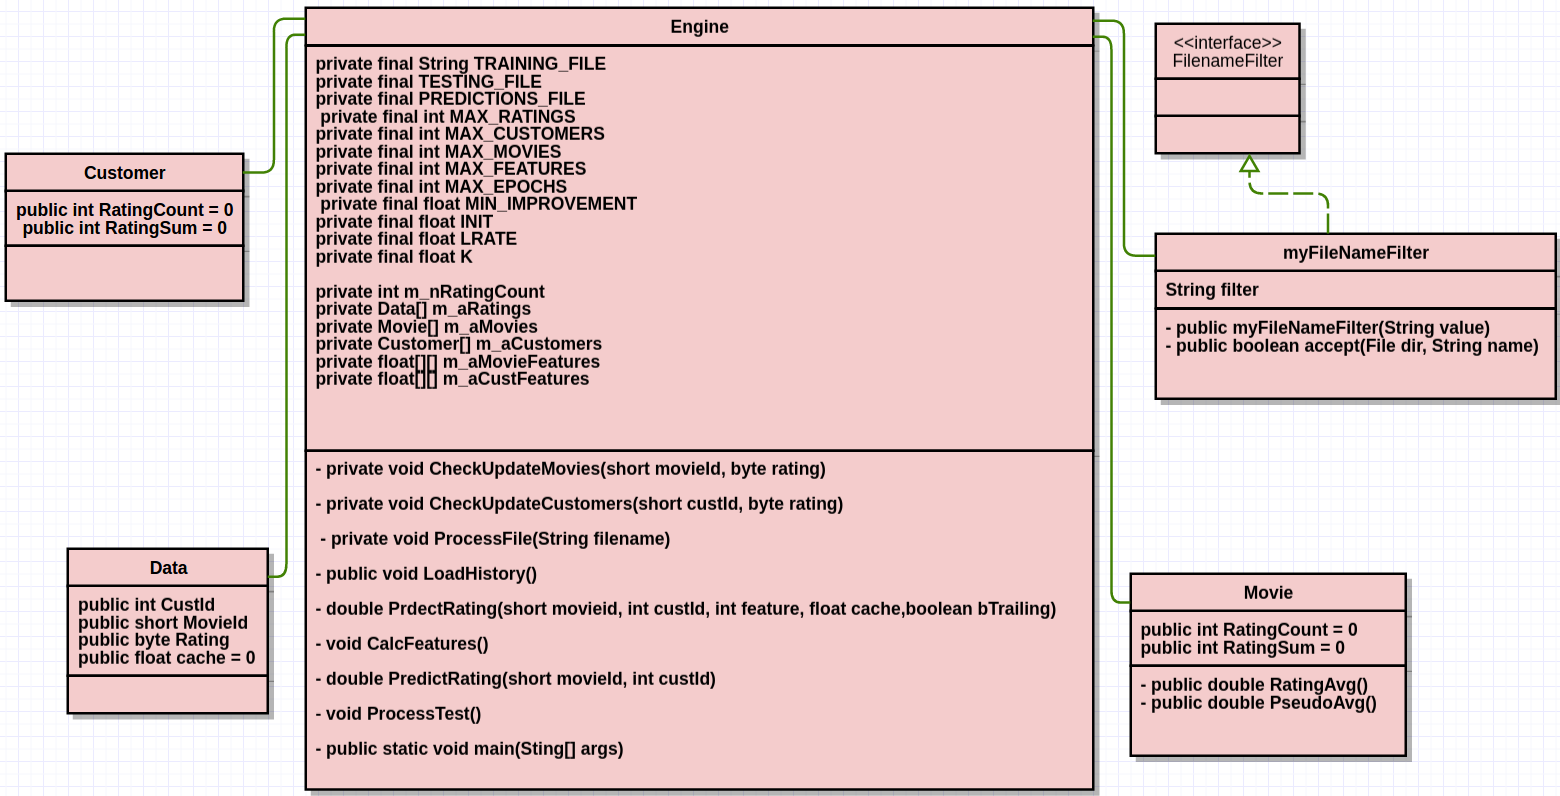
\includegraphics[width=18cm]{arxitektonikodiagramma1}

\vspace{10mm} 

Ακολουθεί το διάγραμμα που αντικατοπτρίζει την υλοποίηση του παράλληλου κώδικα σε \textlatin{Java}.

\vspace{80mm}

\textbf{Σχήμα 2}.

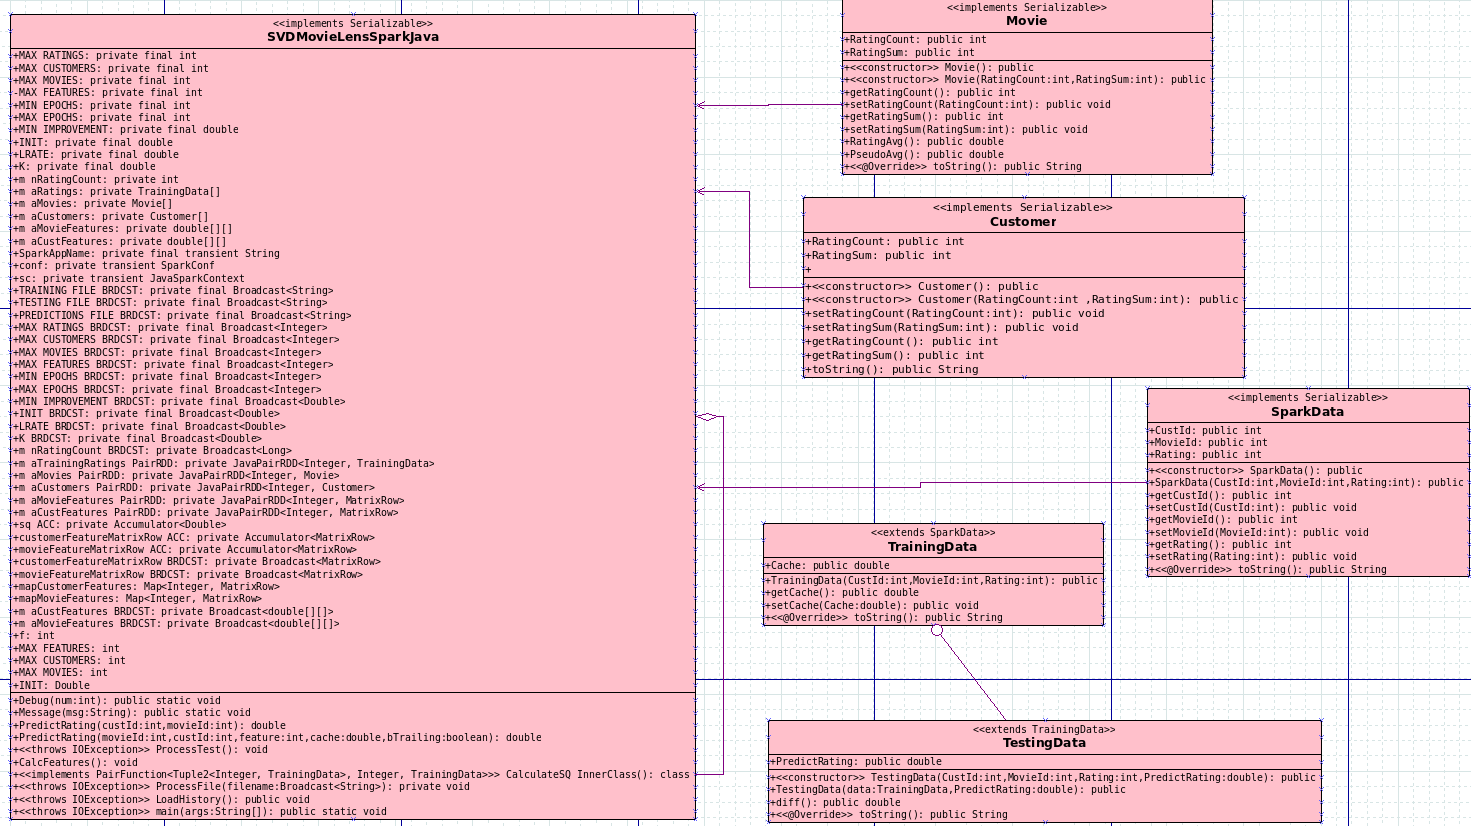
\includegraphics[width=18.5cm]{diagr2}

\vspace{20mm} 

\textbf{\large{4.2 Περιγραφή υποσυστημάτων - λειτουργιών}}

\vspace{4mm} 

\textbf{Περιγραφή ακολουθιακού αλγορίθμου σε \textlatin{C++} με \textlatin{MovieLens Dataset} }

\vspace{2mm}

Αρχικά έπρεπε να γίνει τροποποιήση του αρχικού κώδικα που δόθηκε σε \textlatin{C++} έτσι ώστε να δέχεται ως είσοδο τα \textlatin{MovieLens Dataset}. Καθώς τα \textlatin{dataset} του \textlatin{MovieLens} και του \textlatin{Netflix} διαφέρουν ως προς το πλήθος και τη μορφή των \textlatin{training} αρχείων εισόδου. Τα \textlatin{customer} \textlatin{ID} και \textlatin{movie ID} στο \textlatin{NETFLIX} δεν είναι «κανονικοποιημένα» σε περιοχές [1…] αλλά είναι οι κανονικοί κωδικοί πελάτη και ταινίας, με αποτέλεσμα να μην είναι δυνατή η άμεση χρήση τους σε διευθυνσιοδότηση πινάκων. Παρόλα αυτά έγινε η κατάλληλη μετατροπή στις κρίσιμες \textlatin{functions} που διαβάζουν τα 2 αρχεία. Ο ίδιος που έχει γράψει τον αρχικό κώδικα (\textlatin{http://www.timelydevelopment.com/demos/NetflixPrize.aspx}) αναφέρει ότι ο αλγόριθμος του μπορεί να χρησιμοποιηθεί και να τροποποιηθεί αρκεί να συμπεριληφθεί το μεγάλο σχόλιο που έχει προσθέσει ο ίδιος πάνω από το πρόγραμμα το οποίο περιέχει τις σχετικές ανακοινώσεις και αποδόσεις. Το πρόγραμμα το μετέτρεψα σε περιβάλλον \textlatin{Visual Studio} 13 από τον χώρο εργασίας, καθώς μόνο εκεί είχα πρόσβαση στο εργαλείο αυτό.

Συνεπώς είναι επιτακτική η ανάγκη ύπαρξης αποτελεσμάτων από αυτό το πρόγραμμα έτσι ώστε να ανατρέχω σε αυτά για την επαλήθευση των αποτελεσμάτων που θα εξάγονται από τα 2 επόμενα προγράμματα που θα ακολουθήσουν, το σειριακό και το παράλληλο  πρόγραμμα σε \textlatin{Java}.  

Ουσιαστικά ο αρχικός κώδικας ένα από τα σημεία στα οποία άλλαξε ήταν στα σημεία δήλωσης των μακροεντολών \textlatin{identifier}. Αφαιρέθηκε το \textlatin{FEATURE\_FILE} και το \textlatin{TEST\_PATH} καθώς δεν χρειαζόντουσταν πλέον για το \textlatin{MovieLens}. Τα \textlatin{TRAINING\_PATH, TRAINING\_FILE και PREDICTION\_FILE} διατηρήθηκαν με τα αντίστοιχα αρχεία του \textlatin{MovieLens}. Όπως και τα υπόλοιπα αναγνωριστικά μακροεντολών διατηρήθηκανα και τους ανατέθηκαν οι αντίστοιχες τιμές του \textlatin{MovieLens dataset} των εκατό χιλιάδων βαθμολογιών. Τα τρία \textlatin{structs} που ακολουθούν τροποποιήθηκαν ελάχιστα. Στο \textlatin{struct Movie} οι αρχικά δηλώμενες ως μεταβλητές \textlatin{RatingAvg} και \textlatin{PseudoAvg} αλλάχτηκαν ώστε να είναι δηλωμένες ως μέθοδοι που επιστρέφουν τον ίδιο τύπο δεδομένων με αυτό που είχαν δηλωθεί αρχικά. Στη \textlatin{struct Customer} η μόνη αλλαγή που έγινε είναι ό,τι δεν συμπεριλήφθηκε η δήλωση του \textlatin{member} του \textlatin{CustomerId}. Και στο \textlatin{struct Data} η μόνη μικροαλλαγή που έγινε είναι στο τύπο δήλωσης του \textlatin{member Cache} από \textlatin{float} να είναι \textlatin{doule}. 

Άλλες αλλαγές που έγιναν, είναι ότι πλέον η  μέθοδος \textlatin{ProcessTest}() δεν δέχεται καμία παράμετρο ενώ προηγουμένως δεχόταν σαν παράμετρο το όνομα του αρχείου που παραγόταν με τα αποτελέσματα.

Συνεχίζοντας στην κλάση \textlatin{Engine}, στη δήλωση των δύο μονοδιάστατων πινάκων \textlatin{Movie} και \textlatin{Customer} η μόνη αλλαγή που έγινε είναι ότι δεσμεύτηκε χώρος για ένα στοιχείο παραπάνω. Στους δύο μονοδιάστατους πίνακες \textlatin{m\_aMovieFeatures} και \textlatin{m\_aCustFeatures} η μόνη αλλαγή ήταν να δεσμευτεί μια στήλη παραπάνω και να αλλάξει ο τύπος δεδομένων από \textlatin{float} σε \textlatin{double}. To \textlatin{IdMap} δεν χρειαζόταν για αυτό και δεν συμπερίφθηκε. 

Στον \textlatin{constructor} του \textlatin{Engine} αυτό που αλλάζει είναι οι 2 βρόγχοι που κάνουν επαναλήψεις για τις στήλες των δύο δισδιάστατων πινάκων που προανέφερα καθώς η αρχικοποιήση πλέον ξεκινά από την 1 και μετά και φτάνει μέχρι \textlatin{MAX\_MOVIES+1} και \textlatin{MAX\_CUSTOMERS+1} αντίστοιχα. Αυτή η αλλαγή έγινε διότι στα \textlatin{MovieLens Dataset} δεν υπάρχουν κωδικοί πελάτη και ταινίας με τιμή μηδέν, ξεκινούν από το 1, συνεπώς έπρεπε να γίνει η κατάλληλη τροποποιήση.

Επιπρόσθετα η \textlatin{CalcMetrics}() δεν υπάρχει πλέον καθώς οι λειτουργίες τις υλοποιούνται πλέον στις άλλες κλάσεις και μεθόδους. Η \textlatin{LoadHistory}() πλέον απλά καλεί τη μέθοδο \textlatin{ProcessFile}(), παιρνώντας το \textlatin{TRAINING\_FILE} ως παράμετρο, η οποία περιλαμβάνει και την υλοποιήση της παλιάς \textlatin{LoadHistory}().

Στην νέα \textlatin{ProcessFile}() η \textlatin{wchar\_t pwzBuffer} πλέον δεν χρησιμοποιείται. Επιπλέον δεν μας απασχολεί να διαβάσουμε την πρώτη γραμμή του αρχείου ξεχωριστά, καθώς το νέο \textlatin{dataset} διαφέρει από αυτό του \textlatin{Netflix} στο οποίο, κάθε αρχείο στην πρώτη σειρά είχε τον κωδικό της ταινίας που αντιπροσώπευε. Ενώ τώρα όλα η πληροφοριά είναι συγκεντρωμένη σε ένα αρχείο για όλες τους πελάτες και ταινίες. Συνεπώς στην νέα \textlatin{ProcessFile}() με τον ίδιο τρόπο όπως γινόταν προηγουμένως με ένα \textlatin{pointer} σε \textlatin{FILE} και με την \textlatin{fopen} ανοίγουμε την ροή για διάβασμα σε ένα αρχείο  μέχρι να βρεθεί το τέλος του αρχείου. Μέσα στον επαναληπτικό βρόγχο με την βοήθεια της \textlatin{fscanf} γίνεται  το διάβασμα ενός \textlatin{set} από τις τιμές των \textlatin{data} χρησιμοποιώντας ως \textlatin{delimeter} το \textlatin{tab} για τις 4 στήλες που έχει το αρχείο και στο τέλος κάθε γραμμής χρησιμοποιώ τον ειδικό χαρακτήρα \textlatin{newline} για να προχωρήσει στην επόμενη γραμμή. Στο τέλος κάθε επανάληψης, ο μετρητής \textlatin{m\_nRatingCount} αυξάνεται κατά ένα. Οι τιμές που διαβάζονται, αποθηκεύονται προσωρινά στις βοηθητικές μεταβλητές \textlatin{custId, movieId, rating} και \textlatin{tmp}. Έπειτα αναθέτονται το καθένα στα μέλη κάθε στοιχείου του \textlatin{m\_aRatings} με τη βοήθεια του φορέα πρόσβασης μελών και χρησιμοποιώντας ως \textlatin{index}  το \textlatin{m\_aRatingCount}. Επίσης πριν το τέλος του βρόγχου ενημερώνονται τα στατιστικά για το πλήθος και το άθροισμα των \textlatin{m\_aMovies} και των \textlatin{m\_aCustomers}.  

Η μέθοδος \textlatin{CalcFeatures}() παρέμεινε με ακριβώς την ίδια υλοποιήση. Οι δύο \textlatin{PredictRating}()  για τον γρήγορο υπολογισμό των \textlatin{trailing} αλλά και τον υπολογισμό των τελικών αποτελεσμάτων επίσης παραμείνανε απαράλλαχτες.

Η \textlatin{ProcessTest}() που έχει 2 βασικές λειτουργίες όμως, αλλάζει. Αρχικά πρέπει να φορτώσει ένα από τα αρχεία \textlatin{sample set} που διαθέτει το \textlatin{MovieLens}, αλλά αυτή τη φορά το \textlatin{format} με το οποίο πρέπει να διαβαστούν είναι διαφορετικό. Επομένως ανοίγουμε 1 ροή για διάβασμα στο \textlatin{TESTING\_FILE} και 1 ροή για γράψιμο στο \textlatin{PREDICTION\_FILE} έτσι όπως γινόταν αρχικά αλλά πλέον το διάβασμα του αρχείου γίνεται έτσι όπως συνέβη στο \textlatin{TRAINING\_FILE} δηλαδή διάβασμα της οριοθετημένης γραμμής με \textlatin{tab}, ύστερα αποθηκεύονται προσωρινά οι τιμές που διαβάστηκαν και αμέσως μετά καλείται η \textlatin{PredictRating}() για τον τελικό υπολογισμό των \textlatin{features}. Στη συνέχεια βρίσκουμε το \textlatin{diff} δηλαδή την απόλυτη τιμή της διαφοράς μεταξύ βαθμολογίας και εκτιμώμενης βαθμολογίας για κάθε γραμμή, αθροίζουμε τις διαφορές αυτές και αυξάνουμε τον μετρητή σε κάθε επανάληψη. Πριν το τέλος του βρόγχου, γράφουμε σε κάθε γραμμή στην ίδια μορφή που διαβάσαμε τα άλλα δύο αρχεία, τα αποτελέσματα του \textlatin{custId, movieId, rating, predictrating και diff}.

Μετά το πέρας του βρόγχου γράφουμε στη τελευταία γραμμή του αρχείου τα περιληπτικά στοιχεία, δηλαδή τον αριθμό των προβλέψεων και τον μέσο όρο της απόλυτης τιμής του \textlatin{diff}.

Επιπλέον οι βοηθητικές μεταβλητές που χρησιμοποιούνται στον αρχικό κώδικα δεν χρειάζονται πλέον καθώς δεν υπάρχει ανάγκη για κάποιου είδους \textlatin{parse}.

\vspace{4mm} 

\textbf{Περιγραφή ακολουθιακού αλγορίθμου σε \textlatin{Java} με \textlatin{MovieLens Dataset} }

\vspace{2mm}

Έπειτα ακολούθησε η μετατροπή του  ακολουθιακού κώδικα \textlatin{C++} που δέχεται ως είσοδο \textlatin{Movielens dataset} σε ακολουθιακό κώδικα σε \textlatin{Java} με \textlatin{MovieLens Dataset} επίσης.

Το σειριακό πρόγραμμα, αποτελείται από 5 κλάσεις συνολικά. Αρχικά υπάρχει η κλάση του \textlatin{Customer} στην οποία απλά ορίζονται δύο πεδία και αρχικοποιούντε με 0. Τα  δύο αυτά πεδία είναι το \textlatin{RatingCount} το οποίο κρατάει τον αριθμό των συνολικών ψηφοφοριών που έχει πάρει μέρος ο πελάτης και το \textlatin{RatingSum} που θα αποθηκεύει το συνολικό άθροισμα των βαθμολογιών που έχει δώσει ο πελάτης. 

Η δεύτερη κλάση, είναι η \textlatin{Data}, στην οποία δηλώνονται τέσσερα πεδία, το πρώτο πεδίο είναι το \textlatin{CustId} το οποίο είναι η ταυτότητα του πελάτη, το δεύτερο πεδίο είναι το \textlatin{MovieId} το οποίο είναι η ταυτότητα της ταινίας, το τρίτο είναι το \textlatin{Rating} το οποίο αποτελεί τη βαθμολογία που έχει δώσει ο πελάτης στη ταινία και η \textlatin{Cache} η οποία είναι αρχικοποιημένη με 0.

Τρίτη κλάση, είναι το \textlatin{Movie} στο οποίο δηλώνονται και αρχικοποιούνται με 0 δύο πεδία το \textlatin{RatingCount} το οποίο κρατά το πλήθος των ψηφοφοριών για μια ταινία και το \textlatin{RatingSum} το οποίο κρατά το άθροισμα των βαθμολογιών που έχει πάρει μια ταινία. Επίσης στη κλάση δηλώνονται 2 μέθοδοι το \textlatin{RatingAvg()} που υπολογίζει το μέσο όρο των βαθμολογιών και το \textlatin{PseudoAng()} το οποίο υπολογίζει το ψευδο-μέσο όρο. Και τα 2 προηγουμένως υπολογίζονται χρησιμοποιώντας το \textlatin{RatingCount} και το \textlatin{RatingSum} αλλά κάνοντας διαφορετική πράξη.

Τέταρτη κλάση, είναι το \textlatin{myFileNameFilter} το οποίο υλοποιεί ένα \textlatin{interface} που ονομάζεται \textlatin{FilenameFilter} και χρησιμοποιείται για το φιλτράρισμα λιστών καταλόγων. Στη κλάση αυτή δηλώνεται μια μεταβλητή \textlatin{filter} και υλοποιούνται ο \textlatin{constructor} του \textlatin{myFileNameFilter} και η μέθοδος \textlatin{accept} η οποία παίρνει σαν παραμέτρους το μονοπάτι για το αρχείο και το όνομά του έτσι ώστε να φιλτραριστεί το αρχείο και να επιστρέψει η μέθοδος \textlatin{true} ή \textlatin{false}. 

Πέμπτη κλάση, είναι η \textlatin{Engine} στην οποία δηλώνονται ολόκληρα τα μονοπάτια για το \textlatin{u.data} το οποίο αποτελεί το \textlatin{training file} με όλες τις βαθμολογίες, \textlatin{u1.test} το οποίο αποτελεί το \textlatin{testing fie} και το \textlatin{u1.predictions} το οποίο αποτελεί το \textlatin{predictins file} όπου γράφονται τα αποτελέσματα. Έπειτα ακολουθεί η δήλωση του μέγιστου αριθμού βαθμολογιών, πελατών, ταινιών, features και εποχών καθώς επίσης και ο ελάχιστος αριθμός εποχών.

Στη συνέχεια, ορίζονται ο ελάχιστος δείκτης βελτίωσης του \textlatin{feature}, η αρχική τιμή των \textlatin{features}, η παράμετρος ποσοστιαίας εκμάθησης και η παράμετρος κανονικοποιήσης που χρησιμοποείται για την ελαχιστοποιήση της περιγραφής του τυχαίου σφάλματος ή θορύβου. Μετά ακολουθεί η δήλωση ενός \textlatin{counter} ο οποίος αναλαμβάνει να αποθηκεύει τον τρέχων αριθμό των φορτωμένων βαθμολογιών, ένας μονοδιάστατος πίνακας με τα δεδομένα των βαθμολογιών, ένας άλλος μονοδιάστατος πίνακας με τις μετρικές των ταινιών (πλήθος και άθροισμα) και ένας ακόμα μονοδιάστατος πίνακας με τις μετρικές των πελατών.

Τελικά, δηλώθηκαν δύο δυσδιάστατοι πίνακες, ο πρώτος αποθηκεύει τα \textlatin{features} με βάση τις ταινίες και ο δεύτερος αποθηκεύει τα \textlatin{feautures} με  βάση τους πελάτες. Μετά τη δήλωση των πεδίων, ακολουθεί η δήλωση του \textlatin{constructor} στον οποίο γίνται η αρχικοποιήση του \textlatin{counter} με τον τρέχων αριθμό φορτωμένων βαθμολογιών και με εμφωλευμένους επαναληπτικούς βρόγχους γίνεται η αρχικοποιήση των 2 προηγούμενων δυσδιάστατων πινάκων.

Ύστερα, ακολουθεί η δήλωση των μεθόδων, πρώτη μέθοδος είναι η \textlatin{CheckUpdateMovies}() η οποία παίρνει σαν είσοδο δύο παραμέτρους, τη ταυτότητα της ταινίας και τη βαθμολογία της, εξετάζει να δει αν μια ταυτότητα ταινίας υπάρχει ήδη και ανανεώνει τις μετρικές της ταινίας αυτής, αν δεν υπάρχει τότε πρώτα δημιουργεί μια ταινία με τη καινούρια ταυτότητα και ακολούθως αυξάνει τις μετρικές της. Δεύτερη μέθοδος είναι η \textlatin{CheckUpdateCustomers}() η οποία επίσης παίρνει 2 παραμέτρους, τη ταυτότητα του πελάτη και τη βαθμολογία του και εξετάζεται αν υπάρχει ήδη αυτή η ταυτότητα του πελάτη στο μονοδιάστατο πίνακα \textlatin{m\_aCustomers}[] και ανανεώνονται οι μετρικές του. Διαφορετικά αν δεν υπάρχει δημιουργείται νέος πελάτης με αυτή την ταυτότητα και αυξάνονται οι μετρικές του.

Μετέπειτα, ακολουθεί η μέθοδος \textlatin{ProcessFile}() η οποία παίρνει μια παράμετρο, το μονοπάτι του αρχείου \textlatin{training file}, και γίνεται ανάγνωση του αρχείου με τη βοήθεια του \textlatin{BufferedReader} και \textlatin{Scanner}, των 3 πεδίων που μας ενδιαφέρουν, της ταυτότητας του πελάτη, της ταινίας και της βαθμολογίας ανά γραμμή χρησιμοποιώντας ως \textlatin{delimeter} το \textlatin{tab}. Στη συνέχεια γίνεται ανανέωση των μετρικών του πίνακα με τις βαθμολογίες με βάση τις τιμές που διαβάσαμε από το αρχείο για μια γραμμή. Έπειτα καλούνται οι μέθοδοι \textlatin{CheckUpdateMovies}() και \textlatin{CheckUpdateCustomers}() για την ανανέωση των δικών τους στατιστικών. Τέλος αυξάνεται ο \textlatin{counter} με τον τωρινό αριθμό φορτωμένων βαθμολογιών. Η διαδικασία που περιγράφτηκε υλοποιείται κάθε φορά που διαβάζεται νέα γραμμή από τον \textlatin{inputStream} ο οποίος αποτελεί ένα \textlatin{BufferedReader}. Σε περίπτωση που η προηγούμενη διαδικασία δεν πετύχει, τυπώνεται ένα μήνυμα λάθους στο χρήστη που τον ενημερώνει για την αποτυχία στο άνοιγμα του αρχείου. Τελικά ανεξάρτητα αν πετύχει η διαδικασία ή όχι μπαίνουμε στο μπλοκ \textlatin{Finally} όπου σταματάμε τη ροή του \textlatin{BufferedReader} και του \textlatin{Scanner}. 

Επόμενη μέθοδος, είναι η  \textlatin{LoadHistory}(), η οποία απλά καλεί τη προηγούμενη \textlatin{ProcessFile}() παιρνώντας της ως παράμετρο, το μονοπάτι για το αρχείο \textlatin{training file}. 

'Επειτα υλοποιείται η μέθοδος \textlatin{PredictRating}()  στην οποία περνιούνται πέντε παράμετροι ως είσοδος, τη ταυτότητα της ταινίας και του πελάτη, το \textlatin{feature}, τη \textlatin{cache} και το \textlatin{bTrailing} το οποίο είναι προαιρετικό για τον υπολογισμό νέας τιμής για τη \textlatin{cache}. Στην αρχή ελέγχεται η \textlatin{cache}, αν έχουμε παλιά \textlatin{features} τότε παίρνουμε την \textlatin{cached} τιμή αλλιώς επιλέγεται το 1 ως η προτεινόμενη τιμή για το μέσο.
'Επειτα υπολογίζεται το γινόμενο του \textlatin{feature} ως προς τη ταυτότητα της ταινίας με το \textlatin{feature} ως προς τη ταυτότητα του πελάτη και τελικά προστίθεται στη μεταβλητή \textlatin{sum}, ουσιαστικά προστίθεται η συμμετοχή του τωρινού \textlatin{feature}. Στις ακραίες περιπτώσεις όπου η βαθμολογία είναι πάνω από 5 τότε στο \textlatin{sum} ανατίθεται η τιμή 5 και στη περίπτωση που η βαθμολογία είναι κάτω από 1 τότε ανατίθεται η τιμή 1 στο \textlatin{sum}. Τελικά η \textlatin{PredictRating}() επιστρέφει το \textlatin{sum}. 

Επόμενη μέθοδος, είναι η \textlatin{CalcFeatures}() στην οποία δηλώνονται η ταυτότητα του πελάτη και της ταινίας και αρχικοποιείται η τελευταία όπως και ένας \textlatin{counter} με 0 μαζί με κάποιες άλλες βοηθητικές μεταβλητές για τους επαναληπτικούς βρόγχους. Έπειτα, δηλώνεται ένα αντικείμενο τύπου \textlatin{Data} το \textlatin{rating}, η μεταβλητή δείκτη σφάλματος και μέσης τετραγωνικής ρίζας σφάλματος. Στη συνέχεια, αρχικοποιείται η μεταβλητή της ρίζας του μέσου τετραγωνικού σφάλματος με 2 και η τελευταία μεταβλητή ρίζας του τετραγωνικού σφάλματος με 0. Στη συνέχεια σκανάρονται όλα τα \textlatin{Features} και αναθέτονται τα πεδία του \textlatin{rating} σε αντίστοιχες τοπικές μεταβλητές της μεθόδου έτσι ώστε να υπολογιστεί στη συνέχεια η βαθμολογία και ο δείκτης σφάλματος για τον ελάχιστο αριθμό των εποχών ή μέχρι ωσότου να σταματήσει να γίνεται σημαντική πρόοδος, δηλαδή η διαφορά του δείκτη μέσης τετραγωνικής ρίζας σφάλματος με τον ελάχιστο δείκτη βελτίωσης να είναι μικρότερος του δείκτη ρίζας μέσου τετραγωνικού σφάλματος. Επίσης στην προηγούμενη επαναληπτική διαδικασία γίνονται \textlatin{cache off} οι προηγούμενες τιμές αποθηκεύοντας σε δύο βοηθητικές μεταβλητές τις \textlatin{cf} και \textlatin{mf}  των \textlatin{features} καθώς θα χρειαστούν στην συνέχεια των εφμωλευμένων επαναληπτικών βρόγχων για τον υπολογισμό των νέων τιμών των \textlatin{features} με βάση τους πελάτες και τους τις ταινίες. Πριν το τέλος του δεύτερου εμφωλευμένου βρόγχου, γίνεται ο υπολογισμός της ρίζας του μέσου τετραγωνικού σφάλματος. Μπορεί να τυπωθεί προαιρετικά αυτή η πληροφορία για αυτό έχει προστεθεί σε σχόλια η εντολή εκτύπωσης. Τελικά, συνεχίζοντας στο τελευταίο κομμάτι του δεύτερου εμφωλευμένου βρόγχου ακολουθεί ένας άλλος \textlatin{cache off} οι παλιές προβλέψεις για τις βαθμολογίες καλώντας επαναληπτικά τη μέθοδο \textlatin{PredictRating}() παιρνώντας τις πέντε παραμέτρους που χρειάζεται, για τη ταυτότητα ταινίας και πελάτη, τον δείκτη του \textlatin{feature} τη \textlatin{Cache} του αντικειμένου \textlatin{rating} και τη τελευταία παράμετρο \textlatin{btrailing} να είναι \textlatin{false}. 

Ακολουθεί πάλι η μέθοδος \textlatin{PredictRating}() αλλά σε αυτή τη περίπτωση έχει ως είσοδο μόνο δύο παραμέτρους τη ταυτότητα της ταινίας και του πελάτη, στην οποία γίνεται αρχικοποιήση μια μεταβλητής \textlatin{sum} με το 1. 'Επειτα ακολουθεί ένας επαναληπτικός βρόγχος ο οποίος διατρέχει όλα τα \textlatin{features} των δυσδιάστατων πινάκων \textlatin{m\_aMovieFeatures}[][] και \textlatin{m\_aCustFeatures}[][] για τη συγκεκριμένη ταινία και πελάτη, κρατώντας σταθερό και στους δύο πίνακες τους δείκτες των στηλών δεδομένου των παραμέτρων που έχουν περαστεί με τη κλήση της μεθόδου.
Υπολογίζεται το γινόμενό τους και πριστίθεται στη μεταβλητή  \textlatin{sum}. Στις ακραίες περιπτώσεις που το άθροισμα της βαθμολογίας είναι μεγαλύτερο του 5 αντισταθμίζεται αναθέτοντάς του την τιμή 5 και στην περίπτωση που είναι μικρότερο του ενός του εκχωρείται η τιμή 1. Τέλος επιστρέφεται η τιμή του \textlatin{sum} από τη μέθοδο.      

'Ύστερα, ακολουθεί η μέθοδος \textlatin{ProcessTest}() στην οποία γίνεται ανάγνωση του \textlatin{testing file}, το οποίο όπως αναφέρθηκε και προηγουμένως αποτελεί ένα δείγμα του συνόλου με το ίδιο \textlatin{format} που έχει το \textlatin{u.data}, το οποίο έχει όλο το σύνολο των βαθμολογιών και επίσης γράφονται τα αποτελέσματα στο \textlatin{prediction file}. Αρχικά, αρχικοποιούνται τρία αντικείμενα τύπου \textlatin{BufferedReader}, \textlatin{PrintWriter} και ένας \textlatin{Scanner}, με τη βοήθεια των οποίων θα γίνει η ανάγνωση και το γράψιμο των 2 προηγούμενων αρχείων. Επίσης, αρχικοποιείται η ταυτότητα του πελάτη και της ταινίας, μαζί με την βαθμολογία, την προβλεπόμενη βαθμολογία που θα προκύψει από τις αριθμητικές πράξεις σύμφωνα με την υλοποίηση του κώδικα που έχει υλοποιηθεί σε \textlatin{C++} για το διαγωνισμό του \textlatin{Netflix}. Συνεχίζοντας, γίνεται δήλωση της μεταβλητής \textlatin{diff}, η οποία θα κρατάει την απόλυτη διαφορά μεταξύ της βαθμολογίας και της προτεινόμενης βαθμολογίας, ένας αθροιστής ο οποίος αρχικοποιείται με 0 όπως επίσης και ένας \textlatin{counter}. Γίνεται δήλωση ενός αντικειμένου \textlatin{data} τύπου \textlatin{Data}, και ξεκινάει μια ροή για την ανάγνωσή του με τη βοήθεια του \textlatin{FileReader} και του \textlatin{BufferedReader}. Αμέσως μετά, ξανά με τη βοήθεια των δύο προηγούμενων αντικειμένων ανοίγει το αρχείο \textlatin{testing file} αυτή τη φορά μαζί με τη μέθοδο \textlatin{PrintWriter}, με τη βοήθεια της οποίας θα γίνει το γράψιμο των προβλέψεων στο \textlatin{predictions file}. Με τη μέθοδο \textlatin{radLine}() του αντικειμένου \textlatin{inputStream}, που είναι  τύπου \textlatin{BufferedReader} γίνεται η ανάγνωση κάθε γραμμής των αρχείων, πρώτα γίνεται η ανάγνωση της ταυτότητας του πελάτη και της ταινίας και η βαθμολογία από το αρχείο \textlatin{testing file} και έπειτα καλείται η μέθοδος \textlatin{PredictRating}() για τον υπολογισμό της πρόβλεψης της βαθμολογίας παιρνώντας ως παραμέτρους μόνο τη ταυτότητα της ταινίας και του πελάτη. Μετά, υπολογίζεται η διαφορά της αρχικής βαθμολογίας με αυτήν της προβλεπόμενης σε απόλυτη τιμή και προστίθεται στον αθροιστή και αυξάνεται ο \textlatin{counter} κατά ένα για κάθε γραμμή. Τελικά, γράφονται οι προβλέψεις στο αρχείο \textlatin{predictions file} τοποθετώντας τη ταυτότητα του πελάτη, έπειτα της ταινίας και τη βαθμολογία και μετά την υπολογισμένη προβλεπόμενη βαθμολογία και από δίπλα την απόκλιση που έχει από την αρχική βαθμολογία, χρησιμοποιώντας το \textlatin{tab} ως \textlatin{delimeter}.

Στη περίπτωση που αποτύχει η παραπάνω διαδικασία, γίνεται \textlatin{catch} το σφάλμα για αποτυχία ανοίγματος κάποιου αρχείου και ενημερώνεται ο χρήστης κατάλληλα. Τελικά, στο μπλοκ του \textlatin{finally} που θα εκτελεστεί σε οποιαδήποτε περίπτωση γίνεται το κλείσιμο ροής του αρχείου που έχει ανοίξει ο \textlatin{inputStream} για το \textlatin{testing file}, καθώς επίσης το κλείσιμο του \textlatin{out} που χρησιμοποιήθηκε για το γράψιμο των αποτελεσμάτων στο \textlatin{predictions file}, καθώς επίσης και του βοηθητικού \textlatin{scanner}. Τελικά τυπώνεται στη κονσόλα ένα μύνημα με τον υπολογισμό της μέσης εκτίμησης σφάλματος για τα προηγούμενα αποτελέσματα.   

Τελευταία είναι η μέθοδος \textlatin{main}() από όπου γίνεται η εκκίνηση του προγράμματος. H \textlatin{main}() ξεκινά με τη δήλωση 5 μεταβλητών που θα χρησιμοποιηθούν για την αποθήκευση των χρονικών στιγμών πριν και μετά από τη δημιουργία ενός αντικειμένου τύπου \textlatin{Engine} και τη κλήση κάθε μεθόδου έτσι ώστε να υπολογιστούν οι χρονικές διαφορές στους  και να τυπώσει το πρόγραμμα στη κονσόλα τη χρονική διάρκεια για την εκτέλεση κάθε βήματος ξεχωριστά. Πρώτα ακολουθεί η δημιουργία του αντικειμένου \textlatin{engine} τυπώνεται ο χρόνος για τη δημιουργία του αντικειμένου, μετά ακολουθεί η κλήση της μεθόδου \textlatin{LoadHistory}() του αντικειμένου \textlatin{engine} και έπειτα τυπώνεται η χρονική διάρκεια εκτέλεσής της  σε δευτερόλεπτα. Μετά, γίνεται κλήση της μεθόδου \textlatin{CalcFeatures}() του \textlatin{engine}  και αντίστοιχα εκτυπώνεται η χρονική διάρκεια για την εκτέλεση της μεθόδου. Τελευταία μέθοδος που καλείται είναι η \textlatin{ProcessTest}() του \textlatin{engine} και τελικά τυπώνεται η ο χρόνος εκτέλεσής της καθώς επίσης και ένα ειδοποιητήριο μήνυμα \textlatin{Done} για το τερματισμό του σειριακού προγράμματος. 






\newpage


\begin{center}
\LARGE{5. ΥΛΟΠΟΙΗΣΗ}
\end{center}

\vspace{5mm}

\textbf{\large{5.1 Λεπτομέρειες υλοποίησης}}

\vspace{5mm}

\textbf{Περιγραφή παράλληλου αλγορίθμου σε \textlatin{Java} στο \textlatin{Apache Spark} με \textlatin{MovieLens Dataset} }

\vspace{2mm}

Πριν την υλοποιήση του παράλληλου προγράμματος ακολούθησε μια διαδικασία εξοικείωσης με το \textlatin{Apache Spark}. Διάβασα τα σχετικά \textlatin{Documentation} από το \textlatin{site} του \textlatin{Spark}, όπως \textlatin{Spark Overview, Quick Start, Spark Programming Guide, API Docs (Java), Spark Examples (Java), Cluster Mode Overview, Spark Standalone Mode} κτλπ. Μετά ακολούθησε εξοικίωση με το \textlatin{Scala Shell} για την εκτέλεση αλληλεπιδραστικών παραδειγμάτων. Επιπλέον διάβασα αρκετές διαφορές ανάμεσα στις δυνατότητες της \textlatin{Scala} και της \textlatin{Java}. Πχ. Η \textlatin{parallelize} του \textlatin{sparkContext} της \textlatin{Scala} κάνει απευθείας μετατροπή μήτρες, ενώ η αντίστοιχη μέθοδος του \textlatin{javaSparkContext} απαιτεί μονοδιάστατο πίνακα \textlatin{(vector)}.
Κατανόηση της παραλληλοποίησης μέσω \textlatin{Spark (RDD, Broadcast variables} και \textlatin{Accumulator variables} και \textlatin{tranformations/actions σε RDDs}). Επιλογή κατάλληλων δομών δεδομένων σε \textlatin{Spark Java} στις οποίες θα μετατραπούν οι δομές δεδομένων του ακολουθιακού κώδικα \textlatin{Java}.

Συγκεκριμένα ο πίνακας \textlatin{Ratings} μετατράπηκε σε \textlatin{Broadcast RDD variable} για βελτιστοποίηση της επικοινωνίας. 
Διάφορες σταθερές \textlatin{(static final)} μεταβλητές μετατράπηκαν σε \textlatin{Broadcast variable} αντίστοιχου τύπου, επίσης για βελτιστοποίηση επικοινωνίας. 

\\
Δεν υπάρχει παραλληλοποιήσιμη \textlatin{R/W} δομή που να υποστηρίζει δισδιάστατους πίνακες. Αυτό οφείλεται στην \textlatin{immutable}(αμετάβλητη) φύση των \textlatin{RDD} που είναι και η βασική παραλληλοποιήσιμη δομή στο \textlatin{Apache Spark}. Έγιναν απόπειρες υλοποίησης της παραλληλοποίησης με δικής μου έμπνευσης κλάσεις.
Αυτές οι απόπειρες έχουν συμπεριληφθεί στον κώδικα αλλά δεν καλούνται από την \textlatin{main}() και επομένως δεν εκτελούνται.

\\
Τα σημεία του κώδικα-αλγορίθμου στα οποία εντόπισα δυνατότητα να επιτευχθεί απευθείας παραλληλοποίηση ήταν τρία, τα οποία είναι τα εξής:

\begin{enumerate}
\item Το διάβασμα του αρχείου δεδομένων.
\item Ο υπολογισμός των \textlatin{prediction ratings} για το \textlatin{test file} με υπολογισμένους ήδη τους πίνακες \textlatin{customer} και \textlatin{movie features}.
\item Το γράψιμο του αρχείου αποτελεσμάτων.
\end{enumerate}
\\
Αρχικά λοιπόν το παράλληλο πρόγραμμα αποτελείται από τις εξής κλάσεις, \textlatin{Customer, Movie, SparkData, TrainingData, TestingData} και \textlatin{SVDMovieLensSparkJava}. Η εκκίνηση του προγράμματος γίνεται από την \textlatin{main}() η οποιά εμπεριέχεται στην \textlatin{SVDMovieLensSparkJava}. Όλες οι κλάσεις κάνουν \textlatin{implement} το \textlatin{Serializable} έτσι ώστε να εκτεθούν δημόσια οι λεπτομέρειες όλων των κλάσεων. Χρησιμοποιεί ένα \textlatin{universal identifier} για κάθε \textlatin{Serializable class} ο οποίος κατά τη διάρκεια του \textlatin{deserialization} βοηθά στο να εξασφαλιστεί ότι η φορτωμένη κλάση αντιστοιχεί ακριβώς σε ένα \textlatin{serialized object}. Αν δεν βρεθεί αντιστοιχία τότε ρίχνει \textlatin{InvalidClassException}. 


\rule{17cm}{0.1cm}

\begin{listing}[ht]
\textlatin{\inputminted{java}{docu1.java}}
\end{listing}


\rule{17cm}{0.1cm}


Συνεχίζοντας, στην κλάση του \textlatin{Customer} δηλώνονται και αρχικοποιούνται με μηδέν δύο \textlatin{data members} το \textlatin{RatingCount} και το \textlatin{RatingSum}. Υπάρχει ο \textlatin{default constructor} που απαιτείται για το \textlatin{Serialization} και ο δεύτερος \textlatin{constructor} που αναθέτει τις τιμές που παίρνει σαν παραμέτρους στο \textlatin{RatingCount} και το \textlatin{RatingSum} αντίστοιχα. Έπειτα ακολουθούν οι \textlatin{setters} και \textlatin{getters} για τα μέλη. Τελικά δηλώνεταιη μέθοδος \textlatin{toString}() που αναλαμβάνει να τυπώσει τα προηγούμενα πεδία με τις τιμές τους. 


Έπειτα ακολουθεί η κλάση \textlatin{Movie} στην οποία επίσης δηλώνονται και αρχικοποιούνται με μηδέν τα δύο δικά της \textlatin{data members}, \textlatin{RatingCount} και \textlatin{RatingSum}. Στην συνέχεια δημιουργούνται οι δύο constructor καθώς επίσης οι \textlatin{setters} και οι \textlatin{getters} των μελών. Μετά ακοουθούν η μέθοδος \textlatin{RatingAvg}() που υπολογίζει τον μέσο όρο των βαθμολογιών που έχει πάρει μια ταινία και την \textlatin{PseudoAvg}() που υπολογίζει αντίστοιχα τον ψεύδο-μέσο όρο μιας ταινίας. Τελικά η \textlatin{toString}() τυπώνει τα πεδία και τις αντίστοιχες τιμές τους.



Έπειτα ακολουθεί η κλάση \textlatin{SparkData}, στην οποία δηλώνονται τρία \textlatin{data members} το \textlatin{CustId}, το \textlatin{MovieId} και το \textlatin{Rating}. Μετά ακολουθούν ο \textlatin{default constructor} και ο \textlatin{constructor} που τις αναθέτει τιμές των παραμέτρων που παίρνει στα πεδία της κλάσης. Ύστερα ακολουθούν οι \textlatin{setters} και οι \textlatin{getters}  των πεδίων της κλάσης. Στο τέλος υπάρχει η αντίστοιχη \textlatin{tostring}() μέθοδος που τυπώνει τα πεδία και τις τιμές των \textlatin{CustId, MovieId} και \textlatin{Rating}.



Μετέπειτα ακολουθεί η \textlatin{TrainingData} κλάση, η οποία κληρονομεί την
κλάση \textlatin{SparkData} με όλα τα πεδία και μεθόδους της. Επιπλέον δηλώνεται
και αρχικοποιείται με μηδέν το πεδίο \textlatin{Cache}. Έπειτα ο \textlatin{constructor} της \textlatin{TrainingData}  καλεί τον πατρικό \textlatin{constructor} χρησιμοποιώντας την \textlatin{super}. Ακολουθούν ο \textlatin{setter} και textlatin{getter} για την \textlatin{Cache}. Τελικά υπάρχει η μέθοδος \textlatin{toString}() που τυπώνει τα πεδία της πατρικής κλάσης μαζί με την \textlatin{Cache}.



Στη συνέχεια έρχεται η \textlatin{TestingData} που κληρονομεί με την σειρά της την \textlatin{TrainingData} κλάση. Δηλώνεται ως \textlatin{data member} το \textlatin{PredictRating} και στην συνέχεια ακολουθούν οι \textlatin{constructor} της κλάσης που με την σειρά τους καλούν με την βοήθεια της \textlatin{super} τον πατρικό τους \textlatin{constructor}. Ο πρώτος \textlatin{constructor} παίρνει σαν παράμετρο το \textlatin{CustId, MovieId, Rating} και \textlatin{PredictRating} και ο δεύτερος παίρνει δύο παραμέτρους το \textlatin{TrainingData} και το \textlatin{PredictRating}. Μετά ακολουθεί η μέθοδος \textlatin{diff}() που υπολογίζει και επιστρέφει την απόλυτη τιμή της διαφοράς μεταξύ βαθμολογίας και εκτιμώμενης βαθμολογίας. Τελικά ακολουθεί η \textlatin{toString}() της \textlatin{TestingData} που με την σειρά της θα χρησιμοποιηθεί για να γραφτούν τα αποτελέσματα στο αρχείο αποτελεσμάτων.

Τελευταία κλάση είναι η \textlatin{SVDMovieLensSparkJava}, αρχικά δηλώνονται ο μέγιστος αριθμός βαθμολογιών, πελατών και ταινιών σε ολόκληρο το \textlatin{training set}. Έπειτα δηλώνονται ο μέγιστος αριθμός των \textlatin{feature} που είναι να χρησιμοποιηθούν καθώς επίσης και ο μέγιστος και ελάχιστος αριθμός των εποχών ανά \textlatin{feature}. Δηλώνονται επίσης και ο δείκτς ελάχιστης βελτίωσης που απαιτείται για να συνεχιστεί το τρέχον \textlatin{feature} και η τιμή αρχικοποιήσης για τα \textlatin{features} καθώς επίσης η παράμετρος του ρυθμού εκμάθησης και η παράμετρος κανονικοποιήσης που χρησιμοποιείται για την ελαχιστοποιήση της υπερπροσαρμογής. Επιπλέον δηλώθηκε το πεδίο που θα μετράει τον τωρινό αριθμό των φορτωμένων βαθμολογιών. Επίσης δηλώθηκαν οι τρεις μονοδιάστατοι πίνακες που κρατάνε τις πληροφορίες των βαθμολογιών, τις μετρήσεις για τις ταινίες και τις μετρήσεις για τους πελάτες αλλά και οι δισδιάστατοι πίνακες που κρατάνε τα \textlatin{features} ανά ταινία και ανά πελάτη.

Τα πεδία που δηλώθηκαν μέχρι στιγμής υπήρχαν και στη σειριακή εκδοχή αλλά χρησιμοποιούνται και στο παράλληλο πρόγραμμα για την εκτέλεση της μεθόδου \textlatin{CalcFeatures}(), τώρα ακολουθούν τα πεδία που χρησιμοποιούνται από τις μεθόδους που εκτελούνται παράλληλα. Αρχικά δηλώνεται και ανατίθεται το όνομα της εφαρμογής του \textlatin{Spark} προγράμματος, μετά δηλώνεται η σύνδεση \textlatin{spark context} στο \textlatin{Spark cluster} που θα χρησιμοποιηθεί στην συνέχεια για την δημιουργία \textlatin{RDDs, accumulators} και \textlatin{broadcast variables} σε εκείνο τον \textlatin{cluster} και το \textlatin{spark conf} που χρησμιμοποιείται από το προηγούμενο το οποίο επιτρέπει την ρύθμιση ορισμένων κοινών ιδιοτήτων. Στη συνέχεια δηλώνονται τρεις \textlatin{broadcast variables} το \textlatin{TRAINING\_FILE\_BRDCST}, το \textlatin{TESTING\_FILE\_BRDCST} και το \textlatin{PREDICTIONS\_FILE\_BRDCST} έτσι ώστε κάθε κόμβος να έχει ένα αντίγραφο του \textlatin{input dataset} με έναν αποδοτικό τρόπο. Με τον ίδιο τρόπο δηλώνονται και όλα τα προηγούνενα πεδία που αφορούν το σειριακό κομμάτι με εξαίρεση βέβαια τους 3 μονοδιάστατους και τους δύο δισδιάστατους πίνακες. Οι πίνακες πλέον έχουν δηλωθεί ως \textlatin{JavaPairRDDs} έτσι ώστε να φέρουμε τα δεδομένα σε μορφή \textlatin{key-value RDDs} που θα δώσουν στην συνέχεια την δυνατότητα εκτέλεσης συναθροίσεων, ομαδοποίηση δεδομένων με το ίδιο κλειδί και ομαδοποιήση δύο διαφορετικών \textlatin{RDDs}. Και στους πέντε πίνακες στη θέση του \textlatin{key} παίρνουν \textlatin{Integer generic data type}, ενώ στη θέση του \textlatin{value} οι τρεις μονοδιάστατοι παίρνουν αντικείμενα τύπου \textlatin{TrainingData, Movie} και \textlatin{Customer} ενώ οι δύο δισδιάστατοι στη θέση του value έχουν δηλωθεί έτσι ώστε να δέχονται \textlatin{MatrixRow} δηλαδή ένα \textlatin{row oriented} κατανεμημένο πίνακα χωρίς να έχουν κάποια σημασία οι δείκτες σειράς. Έπειτα ακολούθησε η δήλωση τριώ \textlatin{accummualator} έτσι ώστε με ασφάλεια να ενημερώνονται οι μεταβλητές για τον υπολογισμό του \textlatin{sq} και για τον υπολογισμό των \textlatin{Featureture} των πελατών και των ταινιών όταν η εκτέλεσή τους θα γίνεται ξεχωριστά σε όλους τους \textlatin{worker} κόμβους στο \textlatin{cluster} . Δηλώθηκαν πεδία επίσης για τον υπλογισμό των \textlatin{Featureture} των πελατών και των ταινιών αλλά με τη διαφορά τώρα ότι είναι δηλωμένες ως \textlatin{Broadcast}. Μετά ακολουθεί η δήλωση δύο \textlatin{Map} του \textlatin{mapCustomerFeatures} και του \textlatin{mapMovieFeatures}. Και τελικά δηλώνονται δύο δισδιάστατοι πίνακες \textlatin{broadcast} που  αποθηκεύουν τα \textlatin{feature} ανά \textlatin{Movie} και \textlatin{Customer}. 
 
Στην συνέχεια φτιάχτηκαν δύο μέθοδοι η \textlatin{Debug} και η \textlatin{Message} οι οποίες αποτέλεσαν τα δύο βασικά μου εργαλεία για την αποσφαλμάτωση του κώδικα κατά την διάρκεια της ανάπτυξης, αφού το ίδιο το \textlatin{Apache Spark} δεν υποστηρίζει κάποιο \textlatin{debugging} σύστημα.

\rule{17cm}{0.1cm}

\textlatin{\inputminted{java}{docu7.java}}

\rule{17cm}{0.1cm}


Μετέπειτα, ακολουθεί ο \textlatin{constructor} της \textlatin{SVDMovieLensSparkJava} μέσα στον οποίο γίνεται δημιουργία του \textlatin{Spark Configuration Object}. Είχε γίνει μια απόπειρα να χρησιμοποιηθεί μιας δικιάς μου \textlatin{custom} έκδοσης \textlatin{Kryo Registrator} για βελτιστοποιήση στον χρόνο η οποία τελικά λειτουργούσε αλλά μόνο όσο έκανα απόπειρες για παραλληλοποιήση της μεθόδου της \textlatin{CalcFeatures}() η οποία και τελικά απέτυχε για τους λόγους που έχω  καταγράψει αναλυτικά στην ενότητα 7.2 στην οποία μάλιστα παρουσιάζω τμήματα κώδικα συμπεριλαμβανομένου του \textlatin{Kryo Registrator} και των άλλων προσπαθειών, συμπερασματικά χρησιμοποιήθηκε ο \textlatin{default registrator} που παρέχεται από το \textlatin{Spark}. Στην συνέχεια γίνεται αρχικοποιήση του \textlatin{spark context} συμπεριλαμβανομένου και των υπόλοιπων πεδίων που δηλώθηκαν στο τμήμα του \textlatin{Spark Data Members}.

Ύστερα γίνονται \textlatin{cache} οι τιμές των \textlatin{broadcast} μεταβλητών σε τοπικές μεταβλητές έτσι ώστε να επιτευχθεί βελτιστοποιήση στον χρόνο. Στην συνέχεια δημιουργείται ένα \textlatin{RDD} για τον πίνακα με τα \textlatin{customer feature} χρησιμοποιώντας αυτοδύναμη παραγωγή δεικτών. Ακολουθεί ο επαναληπτικός βρόγχος που διατρέχει όλα τα \textlatin{features} για να δημιουργηθεί ένα \textlatin{vector} από όλους τους πελάτες  με την \textlatin{broadcast} τιμή αρχικοποιήσης. Στη συνέχεια το \textlatin{vector} αυτό με τη βοήθεια της \textlatin{parallelize} βοηθά στη δημιουργία μιας παράλληλης συλλογής \textlatin{RDD} από μια υπάρχουσα συναλλαγή.

Σε αυτή τη παράλληλη συλλογή που δημιουργήθηκε υλοποιούμε το \textlatin{transformation zipWithIndex} το οποίο προσφέρει ένα σταθερό \textlatin{indexing}, απαριθμώντας κάθε στοιχείο κατά την αρχική σειρά του. Επειδή όμως οι δείκτες  με αυτό το \textlatin{transformation} εμφανίζονται δεξιά από τις τιμές, κάνουμε επιπρόσθετα ένα ακόμα \textlatin{transformation} το \textlatin{mapToPair} το οποίο επιστρέφει ένα νέο \textlatin{RDD}  εφαρμόζοντας μια \textlatin{function} σε όλα τα στοιχεία του \textlatin{RDD}. Σε αυτή τη περίπτωση η \textlatin{fuction} αυτό που υλοποιεί είναι αντιστροφή των θέσεων των δύο στοιχείων έτσι ώστε ο \textlatin{index} να βρίσκεται από μπροστά. Αυτό επιτυγχάνεται με τη βοήθεια του \textlatin{Tuple2} το οποίο επιτρέπει το ζευγάρωμα δύο αντικειμένων αλλά και των μεθόδων που υποστηρίζει αυτό για να γίνεται πρόσβαση στο πρώτο και δεύτερο αντικείμενο του \textlatin{Tuple2} αλλά και στα επιμέρους πεδία των αντικειμένων αυτών. Τέτοιου είδους προσβάσεις σε στοιχεία \textlatin{Tuple2} γίνονται πολύ συχνά στην συνέχεια.

Έπειτα ακολουθεί η δημιουργία των \textlatin{RDDs} για τον πίνακα με τα \textlatin{Movie Feature}, χρησιμοποιώντας αυτοδύναμη παραγωγή δεικτών. Γίνεται αντίστοιχα η δημιουργία του \textlatin{vector} με όλες τις ταινίες με την \textlatin{broadcast} τιμή αρχικοποιήσης. To \textlatin{vector} μετατρέπεται σε \textlatin{RDD} στο οποίο αντίστοιχα εφαρμόζεται η \textlatin{zipWithIndex} και η \textlatin{mapToPair} έτσι να επιτευχθεί το \textlatin{indexing} που επιθυμούμε έτσι όπως έγινε με το \textlatin{RDD} με τους πελάτες προηγουμένως.


\rule{17cm}{0.1cm}

\textlatin{\inputminted{java}{docu9.java}}

\rule{17cm}{0.1cm}


Τα \textlatin{transformations} πάνω στα \textlatin{RDDs} έγιναν με \textlatin{lambda expression}.


Μετέπειτα έγινε η κατασκευή των \textlatin{maps} από τα \textlatin{RDDs} με τα \textlatin{Customer} και \textlatin{Movie Features}. 

\vspace{5mm}

\rule{17cm}{0.1cm}

\textlatin{\inputminted{java}{docu8.java}}

\rule{17cm}{0.1cm}


Αμέσως μετά γίνεται η αρχικοποιήση των δύο δισδιάστατων πινάκων \textlatin{m\_aMovieFeatures} και \textlatin{m\_aCustFeatures} έτσι όπως γινόταν προηγουμένως και στο σειριακό πρόγραμμα.

Μετέπειτα έρχεται η σειρά της \textlatin{main}() η οποία ουσιαστικά δημιουργεί ένα αντικείμενο τύπου \textlatin{SVDMovieLensSparkJava}, έπειτα καλείται η \textlatin{LoadHistory}, μετά η \textlatin{CalcFeatures} και τελικά η \textlatin{ProcessTest}. Όλες οι μέθοδοι που θα εξηγήσω στην συνέχεια υλοποιήθηκαν παράλληλα εκτός από την \textlatin{CalcFeatures}() η οποία εκτελείται ακολουθιακά και παρέμενει ως έχει. Καταγράφονται οι χρονικές στιγμές πριν και μετά από την εκτέλεση κάθε μεθόδου έτσι ώστε να μετρηθούν και να καταγραφούν οι χρόνοι εκτέλεσης έτσι ακριβώς όπως έγινε και στο σειριακό πρόγραμμα.

Η πρώτη μέθοδος είναι η \textlatin{LoadHistory}() που κάνει \textlatin{throw} για \textlatin{I/O exception}  και απλά καλεί την μέθοδο \textlatin{ProcessFile}() παιρνώντας ως παράμετρο τo \textlatin{TRAINING\_FILE\_BRDCST}.


Έπειτα στην \textlatin{ProcessFile} που και αυτή κάνει \textlatin{throw} για \textlatin{I/O exception} γίνεται δημιουργία ενός αρχικού \textlatin{RDD} από \textlatin{String} από το διάβασμα του \textlatin{training data} αρχείου. Στην συνέχεια γίνεται ο υπολογισμός του αριθμού των βαθμολογιών και τελικά δημιουργείται ένα \textlatin{RDD} για τα στατιστικά του \textlatin{Customer}. Για τη δημιουργία αυτού του \textlatin{RDD} χρησιμοποιώντας τη \textlatin{map} πάνω στο \textlatin{trainingFile} διαβάζεται το αρχείο με το \textlatin{tab} ως \textlatin{delimeter} και το αποτέλεσμα ανατίθεται στο \textlatin{columnsTrainingFile}.


\rule{17cm}{0.1cm}

\textlatin{\inputminted{java}{docu10.java}}

\rule{17cm}{0.1cm}

Στην συνέχεια στο \textlatin{columnsTrainingFile} γίνεται το \textlatin{transformation mapToPair}  έτσι ώστε να επιστραφεί ένα \textlatin{RDD} με τους κωδικούς των πελατών και τις βαθμολογίες του και θα ανατεθεί στο \textlatin{columnsCustomersA\_} το οποίο είναι δηλωμένο ως \textlatin{PairRDD} από \textlatin{Integer} και \textlatin{Integer}.
Μετά στο \textlatin{columnsCustomersA\_} γίνεται \textlatin{transformation reduceByKey} έτσι ώστε να βρεθεί το άθροισμα των βαθμολογιών που έχει δώσει ο κάθε πελάτης συνολικά, τα αποτελέσματα ανατίθονται στο \textlatin{columnsCustomersA } το οποίο αποτελεί ένα \textlatin{PairRDD}. Έπειτα ξανά γίνεται \textlatin{transformation} στο \textlatin{columnsTrainingFile} έτσι ώστε να πάρουμε αυτή τη φορά τους πελάτες και για κάθε πελάτη ανατίθεται στο πεδίο του \textlatin{value} ο αριθμός ένα και τελικά ανατίθενται στο \textlatin{PairRDD} \textlatin{columnsCustomersB\_}. Ύστερα στο \textlatin{columnsCustomersB\_} γίνεται το \textlatin{transformation reduceByKey} έτσι ώστε να βρεθεί το πλήθος των βαθμολογιών που έχει δώσει κάθε πελάτης τα οποία και ανατίθενται στο \textlatin{columnsCustomersB}. Στη συνέχεια γίνεται \textlatin{join} των δύο \textlatin{PairRDDs} \textlatin{columnsCustomersΑ} και \textlatin{columnsCustomersB} έτσι ώστε να επιστραφεί ένα \textlatin{PairRDD} με το \textlatin{key} να είναι \textlatin{Integer} που θα είναι ο κωδικός πελάτη και \textlatin{value} να είναι ένα \textlatin{Tuple2} με \textlatin{key} να είναι \textlatin{Integer} το οποίο θα είναι το πλήθος των βαθμολογιών που έχει δώσει κάθε πελάτης και \textlatin{value} να είναι επίσης \textlatin{Integer} με το άθροισμα των βαθμολογιών που έχει δώσει ο κάθε πελάτης. Το \textlatin{PairRDD} αυτό ανατίθεται στο \textlatin{columnsCustomers}. Και τελικά το \textlatin{columnsCustomers} που προκύπτει αντιστοιχίζεται στο \textlatin{.m\_aCustomers\_PairRDD} το οποίο είναι δηλωμένο ως \textlatin{PairRDD} με \textlatin{Integer} και \textlatin{Customer object}. Συνεπώς στο πεδίο του \textlatin{Integer} αντιστοιχείται ο κωδικός πελάτη και στο \textlatin{Customer object} του οποίου η κλάση έχει δηλωθεί αντιστοιχίζονται τα πεδία \textlatin{RatingCount} και \textlatin{RatingSum} τα οποία και υπάρχουν στο \textlatin{columnsCustomers}.


\rule{17cm}{0.1cm}

\textlatin{\inputminted{java}{docu11.java}}

\rule{17cm}{0.1cm}




Με αντίστοιχη διαδικασία γίνεται και η δημιουργία του \textlatin{RDD} για τα στατιστικά των ταινιών.
Εντοπίζεται το πλήθος και το άθροισμα των βαθμολογιών για κάθε ταινία και τελικά φορτώνται οι κωδικοί των ταινιών, τα πλήθη και τα αθροίσματα των βαθμολογιών ανά ταινία στο \textlatin{m\_aMovies\_PairRD}. Μετέπειτα ακολουθεί η δημιουργία του πίνακα με τις βαθμολογίες από τα \textlatin{Data} αντικείμενα, πάνω στα \textlatin{RDD}  \textlatin{columnsTrainingFile, rddData} και \textlatin{rddIndexedData} γίνονται τα \textlatin{transformations map, zipWithIndex} και   \textlatin{mapToPair} αντίστοιχα και προκύπτει το τελικό \textlatin{m\_aTrainingRatings\_PairRDD} .
 
\rule{17cm}{0.1cm}

\textlatin{\inputminted{java}{docu12.java}}

\rule{17cm}{0.1cm}


\vspace{10mm}

Στην συνέχεια γίνεται ενημέρωση των μελών της σειριακής. έκδοσης. 

\rule{17cm}{0.1cm}

\textlatin{\inputminted{java}{docu16.java}}

\rule{17cm}{0.1cm}


Έπειτα έρχεται η σειρά της \textlatin{CalcFeatures}() η οποία δεν άλλαξε και παραμένει ακολουθιακή, διότι δεν γίνεται να παραλληλοποιηθεί και για αυτό εκτελείται μόνο από τον \textlatin{driver}. Αυτό ουσιαστικά δεν είναι δύσκολο να επιτευχθεί αρκεί να αναλογιστεί κανείς τα εξής ακόλουθα, οτιδήποτε πραγματοποιείται στο εσωτερικό του \textlatin{closure} από  \textlatin{transformations} όπως (\textlatin{map, filter, groupBy, aggregateBy,} κτλπ.) υλοποιείται σε \textlatin{executor} ή σε \textlatin{executors}. Στα προηγούμενα συμπεριλαμβάνονται η ανάγνωση δεδομένων από απομακρυσμένες πηγές ή \textlatin{persistent storage}. Ενώ \textlatin{actions} όπως το \textlatin{count, reduce}, κτλ. συνήθως εκτελούνται και από τον \textlatin{driver} και τους \textlatin{executors}, σε αυτές τις περιπτώσεις ο μεγαλύτερος φόρτος εργασίας αναλαμβάνεται να υλοποιηθεί παράλληλα και μερικά τελευταία βήματα εκτελούνται διαδοχικά στον \textlatin{driver}. Όλα τα υπόλοιπα που κάνουν \textlatin{trigger} ένα \textlatin{action} ή \textlatin{transformation} συμβαίνουν στον \textlatin{driver}. Πιο συγκεκριμένα κάθε ενέργεια που χρειάζεται πρόσβαση στο \textlatin{SparkContext} εκτελείται στον \textlatin{driver}.

Κατόπιν ακολουθεί η αρχικοποιήση των \textlatin{broadcast} πινάκων \textlatin{m\_aCustFeatures\_BRDCST}  και \textlatin{m\_aMovie} \textlatin{Features\_BRDCST} έτσι ώστε να είναι διαθέσιμοι στους \textlatin{executors}.

\vspace{15mm}


\rule{17cm}{0.1cm}

\textlatin{\inputminted{java}{docu3.java}}

\rule{17cm}{0.1cm}



Μετέπειτα έρχεται η σειρά της τελευταίας μεθόδου \textlatin{ProcessTes}() της οποίας οι βασικές λειτουργίες είναι το παράλληλο διάβασμα του \textlatin{test file} και η εξαγωγή του αρχείου με τα αποτελέσματα \textlatin{predictions file} παράλληλα. Αρχικά δηλώνεται ένας μετρητής ο οποίος κρατά τον αριθμό των βαθμολογιών στο \textlatin{test file} και ένας αθροιστής \textlatin{sum} ο οποίος αθροίζει τις απόλυτες τιμές των διαφορών μεταξύ βαθμολογιών και εκτιμώμενων βαθμολογιών. Αργότερα υλοποιείται το διάβασμα του \textlatin{test file} με την \textlatin{textFile} χρησιμοποιώντας ως \textlatin{delimeter} το \textlatin{tab} κρατάω από κάθε γραμμή μόνο τις πληροφορίες από τις πρώτες τρεις στήλες, η χρονοσφραγίδα δεν χρησιμοποιείται και όλα αυτά φορτώνονται στο \textlatin{RDD  c\_testingData\_RDD}.


\rule{17cm}{0.1cm}

\textlatin{\inputminted{java}{docu5.java}}

\rule{17cm}{0.1cm}


Μετά ακολουθεί η μετατροπή του \textlatin{RDD} με τα \textlatin{TrainingData} σε \textlatin{RDD} το \textlatin{testingDataRDD} με τα \textlatin{TestingData}  μαζί με τις προβλέψεις, καλώντας την \textlatin{PredictRating}() και παιρνώντας της ως παραμέτρους τον κωδικό πελάτη και ταινίας. Το μόνο που αλλάζει στην υλοποιήση της \textlatin{PredictRating}() είναι η χρήση των δύο \textlatin{broadcast} δισδιάστατων πινάκων για να γίνεται ο υπολογισμός παράλληλα από όλους τους \textlatin{executors}, στη θέση των δύο παραδοσιακών δισδιάστατων πινάκων έτσι όπως υλοποιούνταν στη σειριακή εκδοχή. Τελικά μετριέται το πλήθος των βαθμολογιών στο \textlatin{testingDataRDD}, γίνεται η άθροιση με την \textlatin{sum} μεταβλητή και γίνεται η αποθήκευση του \textlatin{RDD} στο \textlatin{prediction file} με την \textlatin{saveAsTextFile}. Για την ολοκήρωση του προγράμματος τυπώνονται ο συνολικός αριθμός των προβλέψεων που εξάγονται στο αρχείο και ο δείκτης μέσου όρου της απόλυτης τίμης της διαφοροποιήσης μεταξύ βαθμολογιών και εκτιμώμενων βαθμολογιών το οποίο προκύπτει από τη διαίρεση του \textlatin{sum} με το \textlatin{cnt}.


\rule{17cm}{0.1cm}

\textlatin{\inputminted{java}{docu6.java}}

\rule{17cm}{0.1cm}



\vspace{10mm}


\textbf{\large{5.2 Οθόνες εφαρμογής}}

\vspace{1mm}

Ο λόγος που κρίθηκε αναγκαία η εκτέλεση του αρχικού προγράμματος σε \textlatin{C++} ήταν έτσι ώστε να διαπιστωθεί καλύτερα η λειτουργία του προγράμματος και έτσι ώστε να υπάρχει μια σαφέστερη εικόνα των εξαγόμενων πληροφοριών του προγράμματος που στη συνέχεια χρησιμοποιήθηκε ως πυξίδα για την αντίστοιχη υλοποιήση σε \textlatin{Java}.

 Ακολουθεί η εικόνα από τα αρχεία με τα αποτελέσματα που έχουν εξαχθεί έτσι ώστε να μπορώ να καθοδηγούμαι από αυτά και να μπορώ να τα συγκρίνω και να επαληθεύσω τα αποτελέσματα που προκύπτουν στη συνέχεια από το σειριακό και το παράλληλο πρόγραμμα σε \textlatin{Java}. Επιπλέον τα αποτελέσματα ουσιαστικά  που εξάγονται σε 5 στήλες με \textlatin{tab} αναμεσά τους, είναι οι προηγούμενες πληροφορίες ταυτότητα πελατών και ταινιών, βαθμολογίες που έχουν ανατεθεί για τις ταινίες, εκτιμώμενες βαθμολογίες και τέλος στη τελευταία στήλη απόκλιση εκτιμώμενης βαθμολογίας από την αρχική βαθμολογία.
 
 \vspace{50mm}
 
 
\textbf{Εικόνα 1}



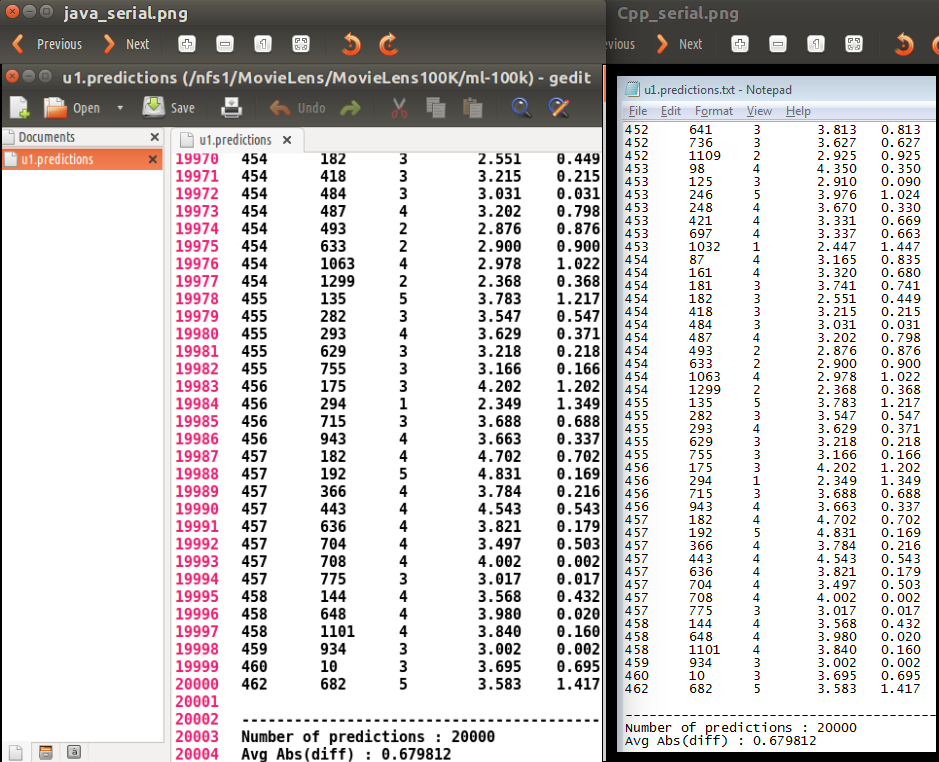
\includegraphics[width=18cm]{sos}

\vspace{3mm}

Από πάνω φαίνονται μαζί τα αποτελέσματα από τα \textlatin{predictions files} που δημιουργήθηκαν από το σειριακό πρόγραμμα σε \textlatin{Java} (αριστερά) και από το σειριακό πρόγραμμα σε \textlatin{C++} (δεξιά) έτσι ώστε να επαληθευτούν τα αποτελέσματα. Παρατηρούμε ότι τα αποτελέσματα και στις 5 στήλες (\textlatin{customer id, movie id, rating, predicted rating, abs(rating - predicted rating)}) είναι ίδια. Καθώς επίσης και ο συνολικός αριθμός των προβλέψεων όπως επίσης και ο μέσος όρος της απόλυτης διαφοράς του \textlatin{rating - predicted rating} είναι ακριβώς ίδια.

\vspace{2mm}


\\

\vspace{5mm}

Ακολουθούν οι οθόνες εφαρμογής από το παράλληλο πρόγραμμα υλοποιημένο σε \textlatin{Java} στο \textlatin{Apache Spark} με το \textlatin{dataset} των 100.000 βαθμολογιών.

Από κάτω ακολουθούν εικόνες από το \textlatin{output} στο \textlatin{directory} του \textlatin{nfs}. Όπως μπορούμε να διαπιστώσουμε η \textlatin{saveAsTextFile()} παράγει ένα φάκελο με το όνομα \textlatin{u1.predictions} ο οποίος μέσα του περιλαμβάνει τα αποτελέσματα σε δύο αρχεία το \textlatin{part-00000} και το \textlatin{part-00001}. 

\vspace{2mm}

\textbf{Εικόνα 2}

\vspace{2mm)

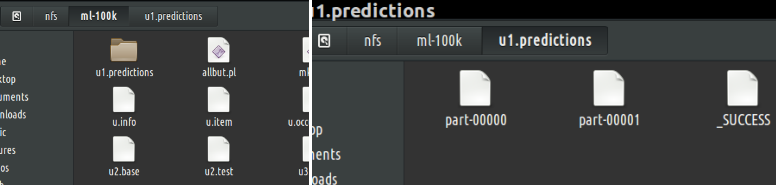
\includegraphics[width=18cm]{sparkpred1}

\vspace{2mm}

Από κάτω φαίνονται μαζί τα αποτελέσματα από τα \textlatin{predictions files} που δημιουργήθηκαν από το παράλληλο πρόγραμμα σε \textlatin{Java} (αριστερά) στο \textlatin{Spark}, το σειριακό πρόγραμμα σε \textlatin{Java} (κέντρο) και από το σειριακό πρόγραμμα σε \textlatin{C++} (δεξιά) έτσι ώστε να επαληθευτούν τα αποτελέσματα. Παρατηρούμε ότι τα αποτελέσματα και στις 5 στήλες (\textlatin{customer id, movie id, rating, predicted rating, abs(rating - predicted rating)}) είναι ίδια. Καθώς επίσης και ο συνολικός αριθμός των προβλέψεων όπως επίσης και ο μέσος όρος της απόλυτης διαφοράς του \textlatin{rating - predicted rating} είναι ακριβώς ίδια.

\vspace{3mm}

\textbf{Εικόνα 3}

\vspace{2mm}

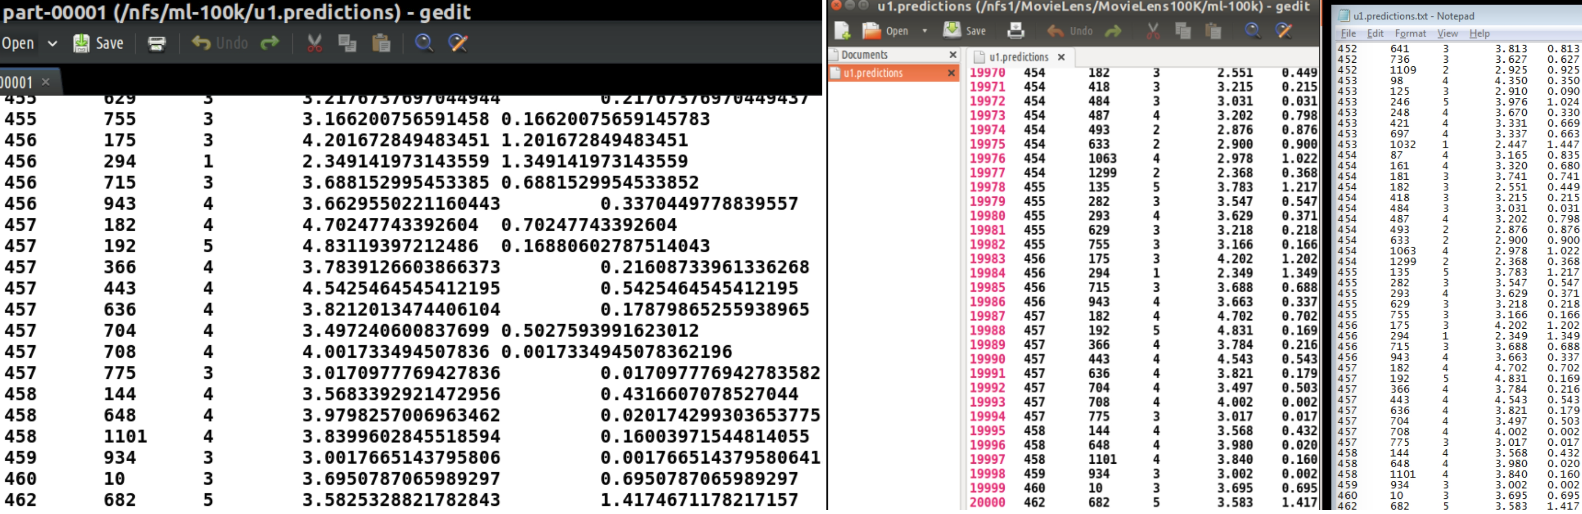
\includegraphics[width=18cm]{sparkpred2}

\vspace{2mm}

Επιπλέον ο λόγος που στο \textlatin{predictions file} του παράλληλου πρόγραμματος μερικά στοιχεία της πέμπτης στήλης δεν είναι στοιχισμένα σωστά όπως τα υπόλοιπα της ίδιας στήλης, αποδίδεται στο γεγονός ότι υπάρχει μεγαλύτερη δεκαδική ακρίβεια στα νούμερα, ωστόσο τα αποτελέσματα που φαίνονται και στα 3 αρχεία είναι ίδια.

\newpage

\vspace{20mm}


\begin{center}
\LARGE{6. ΑΠΟΤΕΛΕΣΜΑΤΑ - ΑΞΙΟΛΟΓΗΣΗ}
\end{center}

\vspace{5mm} 

\textbf{\large{6.1 Μετρικές αξιολόγησης και συγκριτική αξιολόγηση}}


    Ως μέτρο αξιολόγησης για την απόδοση των προγραμμάτων θεωρείται ο χρόνος και τα αποτελέσματα για τα οποία γίνεται αναφορά στην επόμενη παράγραφο.. Ο συνολικός χρόνος εκτέλεσης για το σειριακό πρόγραμμα σε \textlatin{Java} με το μικρό \textlatin{dataset} του \textlatin{MovieLens} των εκατό χιλιάδων βαθμολογιών ήταν 6 \textlatin{seconds}. Αξιοσημείωτο είναι ότι ο χρόνος για την κατασκευή του αντικειμένου engine, για το φόρτωμα του \textlatin{training file} και το γράψιμο των αποτελεσμάτων στο \textlatin{testing file} είναι ίσος με το μηδέν. Όλος ο χρόνος εκτέλεσης του σειριακού προγράμματος εξαρτάται από τον υπολογισμό των \textlatin{features}. Ενώ στο παράλληλο πρόγραμμα ο χρόνος εκτέλεσης  για την κατασκευή του αντίστοιχου \textlatin{engine}  διαρκεί 5 \textlatin{seconds}, για να διαβαστεί το \textlatin{training data } η διάρκεια είναι 3 \textlatin{seconds}, o υπολογισμός των \textlatin{features} 18 \textlatin{seconds} και τελικά το γράψιμο των αποτελεσμάτων 1 \textlatin{second}. Ουσιαστικά όλες οι μέθοδοι του σειριακού προγράμματος εκτελούνται πιο γρήγορα και με μεγάλη διαφορά. Ένας  λόγος στον οποίο μπορεί να αποδοθούν τα προηγούμενα αποτελέσματα είναι στο ότι το κόστος επικοινωνίας μεταξύ του \textlatin{driver} και των \textlatin{executors} είναι πολύ μεγάλο και ξεπερνάει κατά πολύ την χρονική πολυπλοκότητα των λειτουργιών και πράξεων που εκτελούνται στο σειριακό πρόγραμμα. Ένας άλλος λόγος είναι το μέγεθος του \textlatin{dataset} το οποίο είναι μικρό, γεγονός το οποίο δεν βοηθά στο να παραατηρηθεί κάποια βελτιστοποιήση από τη μεριά του παράλληλου προγράμματος. Είναι πιθανό ότι αν το πρόγραμμα ήταν να εκτελεστεί χρησιμοποιώντας το μεγαλύτερο \textlatin{dataset} που υποστηρίζει το \textlatin{MovieLens} για παράδειγμα αυτό των 20 εκατομμυρίων βαθμολογιών  το οποίο είναι διακόσες φορές μεγαλύτερο από αυτό που χρησιμοποείται στη παρούσα εργασία και με την εκτέλεση του σε κατάλληλο περιβάλλον δηλαδή σε κάποιο \textlatin{computer cluster} με υποδομή ευρείας κλίμακας τότε ίσως εκεί πιθανόν να παρατηρούνταν καλύτεροι χρόνοι στο παράλληλο πρόγραμμα γιατί τότε θα υπήρχαν περισσότεροι \textlatin{executors} για να διαμοιραστούν τα \textlatin{tasks} και επιπλέον το \textlatin{dataset} θα ήταν πλέον αρκετά μεγάλο και πλέον ο φόρτος εργασίας θα αυξανόταν δραματικά για το ακολουθιακό πρόγραμμα, πράγμα που σημαίνει ότι ο χρόνος εκτέλεσης του θα αυξανόταν αρκετά. Έγινε μεγάλος πειραματισμός με επιτυχία, μεγαλύτερου μεγέθους \textlatin{datasets}  όπως του ενός εκατομμυρίου βαθμολογιών, των τριών εκατομμυρίων βαθμολογιών και 5 εκατομμυριών βαθμολογιών αλλά και απόπειρα για εκτέλεση με μεγαλύτερα \textlatin{dataset} χωρίς όμως επιτυχία για αυτά που ήταν πάνω από το όριο των 5 εκατομμυρίων, τον λόγο τον αναφέρω στην ενότητα 6.2 . Από τη συγκέντρωση των παραπάνω αποτελεσμάτων παρατηρήθηκαν τα εξής, πράγματι καθώς αυξάνεται το μέγεθος του \textlatin{dataset} ο συνολικός χρόνος εκτέλεσης του παράλληλου προγράμματος είναι μικρότερος από ότι ο συνολικός χρόνος εκτέλεσης για το σειριακό πρόγραμμα σε \textlatin{Java}, αυτό μπορεί να φανεί από τους χρόνους εκτέλεσης με \textlatin{dataset} του ενός εκατομμυρίου και των πέντε εκατομμυρίων. Παρότι σε αυτά τα παραδείγματα σε όλες τις μεθόδους εκτός της \textlatin{CalcFeatures} παρατηρείται ότι οι χρόνοι εκτέλεσης στο σειριακό πρόγραμμα είναι πιο γρήγόροι λόγω της μέγαλης διαφοράς στον χρόνο εκτέλεσης της \textlatin{CalcFeatures} τελικά ο συνολικός χρόνος εκτέλεσης είναι πιο γρήγορος στο παράληλλο πρόγραμμα. Ωστόσο παρατήρησα ότι με dataset των 3 εκατομμυρίων που ανάμεσα στο 1 και 5 το σειριακό πρόγραμμα εκτελείται πιο γρήγορα, από αυτό συμπαιρένω ότι το πρόγραμμα δεν κάνει \textlatin{scale up} ομαλά. Έπίσης ήθελα να τονίσω ότι η ανάπτυξη στο \textlatin{Apache Spark} αποτέλεσε μεγάλη δυσκολία καταρχήν λόγω της άγνωστης πτυχής του για εμένα αλλά και εξαιτίας τη μη ύπαρξης εργαλείου \textlatin{debugger} το οποίο περιόρισε σημαντικά τον τρόπο λειτουργίας μου αλλά και τον εξαναγκασμό μου να δημιουρήσω δικά μου βοηθητικά μηνύματα συνεχώς έτσι ώστε βηματικά να γίνεται η αποσφαλμάτωση του προγράμματος.


\newpage


\textbf{\large{6.2 Αποτελέσματα}}

\vspace{2mm}

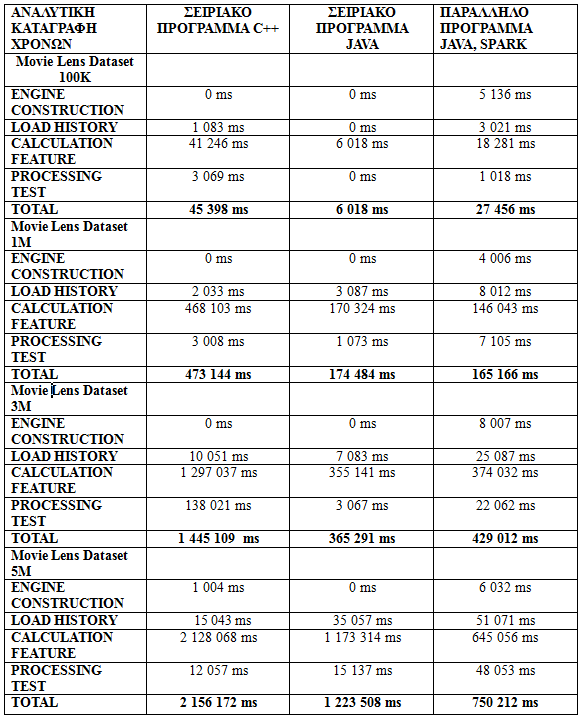
\includegraphics[width=15cm]{table}

\vspace{3mm} 

Όπως μπορούμε να διαπιστώσουμε και από τις οθόνες εφαρμογής που προηγήθηκαν τα αποτελέσματα που παράχθηκαν στα αρχεία \textlatin{predictions files} και από τα 2 προγράμματα σειριακό και παράλληλο σε \textlatin{Java} είναι ακριβώς ίδια με το αρχείο με τα αποτελέσματα που έχουν παραχθεί από το πρόγραμμα σε \textlatin{C++}. Τα αποτελέσματα γράφτηκαν στο αρχείο στην ίδια μορφή, σε 5 στήλες δηλαδή χωρισμένες με ένα \textlatin{tab} ανάμεσά τους. Επίσης ο αριθμός των εξαγόμενων αποτελεσμάτων στα αρχεία είναι ο ίδιος αλλά και ο δείκτης μέσου όρου της απόλυτης τιμής της διαφοράς μεταξύ βαθμολογίας και εκτιμώμενης βαθμολογίας είναι ακριβώς ίδιος. Τα προηγούμενα είχαν τεθεί ως απαιτούμενα για την λειτουργικότητα των προγραμμάτων καθώς χωρίς σωστά αποτελέσματα όλες οι συγκρίσεις χρόνων δεν θα ήταν αξιόπιστες για να αποδωθεί προσοχή σε αυτές.

Στον παραπάνω πίνακα φαίνεται συγκεγκεντρωμένο το σύνολο των αποτελεσμάτων με διαφορετικού μεγέθους \textlatin{dataset}.


Τα αποτελέσματα από πάνω παράχθηκαν μετά από διαδοχικές και επαναληπτικές εκτελέσεις κάθε προγράμματος έτσι ώστε να εξαχθεί ο μέσος όρος των αποτελεσμάτων όσο πιο σωστά γίνεται.

Το σειριακό πρόγραμμα σε \textlatin{Java} και το παράλληλο πρόγραμμα σε \textlatin{Java} στo \textlatin{Spark} εκτελέστηκαν με τα ίδια \textlatin{resources} στον προσωπικό μου υπολογιστή, όπως έχω προαναφέρει. Ωστόσο η εκτέλεση του προγράμματος σε \textlatin{C++} όπως επίσης προανέφερα έγινε σε υπολογιστή από τον χώρο εργασίας μου που έχει εγκατεστημένο \textlatin{Windows 7} λειτουργικό σύστημα και υποστηρίζει το \textlatin{Visual Studio 2013}. Τα αναλυτικά χαρακτηριστικά των υπολογιστών έχουν προαναφερθεί στην ενότητα 2.3 . 

Δοκιμάζοντας σε \textlatin{cluster mode} να τρέξω το παράλληλο πρόγραμμα με \textlatin{dataset} πάνω από 5 εκατομμύρια διαπίστωσα ότι δεν μπορεί να εκτελεστεί λόγω \textlatin{java.lang.OutOfMemoryError:Java heap space}, δηλαδή δεν φτάνει η μνήμη στον \textlatin{driver} για να το εκτελέσει. Ο \textlatin{driver} έχει αρκετή \textlatin{memory} συνολικά 24 \textlatin{GB RAM} αλλά μοιράζονται 4 και 4 στα δύο \textlatin{virtual machines}. Έγινε προσπάθεια για να γίνει η καλύτερη εφικτή οικονομία στα \textlatin{transformations}, επίσης στη διαδικασία ανάπτυξης το ίδιο το \textlatin{Spark} με ανάγκαζε να παραμείνω κάτω από τα 100 \textlatin{MB} και με επίπονη προσπάθεια κατάφερα να περάσει οριακά. Έγινε προσπάθεια και με τον \textlatin{Kryo Seriallizer} αλλά δεν πέτυχε, στην επόμενη ενότητα έχω συμπεριλάβει μεταξύ άλλων και την προσπάθεια αυτή.    

\vspace{20mm} 

\newpage

\begin{center}
\LARGE{7. ΣΥΜΠΕΡΑΣΜΑΤΑ}
\end{center}

\vspace{5mm}

\textbf{\large{7.1 Σύνοψη της προτεινόμενης προσέγγισης με καινοτόμα στοιχεία και θετικά αποτελέσματα }}

\vspace{2mm} 

Τα θετικά αποτελέσματα εν κατακλείδι που προέκυψαν από την παρούσα πτυχιακή εργασία είναι πολλαπλά. Αρχικά έγινε επιτυχημένα η παραμετροποιήση του σειριακού αλγορίθμου στην ίδια γλώσσα προγραμματισμού που είχε υλοποιηθεί αρχικά (\textlatin{C++}) έτσι όπως δίνεται από τον ιστότοπο \textlatin{http://www.timelydeve} \textlatin{opment.com/demos/NetflixPrize.aspx}, (ο οποίος μάλιστα βραβεύτηκε ως ο 3ος καλύτερος στο σχετικό διαγωνισμό του \textlatin{Netflix}). Η παραμετροποιήση έγινε ώστε ο νέος αλγόριθμος να δέχεται ως είσοδο τα \textlatin{dataset} στη μορφή του \textlatin{MovieLens}. Έπειτα έγινε μετατροπή του τελευταίου προαναφερμένου προγράμματος σε γλώσσα προγραμματισμού \textlatin{Java} επίσης σε σειριακή μορφή. Ο χρόνος εκτέλεσης του ακολουθιακού προγράμματος σε \textlatin{Java} με το μικρό \textlatin{dataset} των 100.000 βαθμολογιών ήταν αρκετά μικρός 6 \textlatin{second}. Πράγμα το οποίο δεν ήταν πολύ ενθαρυντικό για τον χρόνο που θα πετύχει το παράλληλο πρόγραμμα. Καθώς εάν παρατηρηθεί βελτιστοποίηση στο συνολικό χρόνο ή σε κάποια μέθοδο ξεχωριστά αυτό θα συμβεί μόνο στα μεγαλύτερα \textlatin{dataset} του \textlatin{MovieLens} αυτά των 10.000.000 βαθμολογιών και 20.000.000 βαθμολογιών. Προχωρόντας, έγινε εφικτή η παραλληλοποίηση του αλγορίθμου (με εξαίρεση τη μέθοδο \textlatin{CalcFeatures}() της οποίας η εκτέλεση όπως εξηγώ αναλυτικά στην αμέσως επόμενη ενότητα δεν μπορεί να παραλληλοποιηθεί σωστά στο \textlatin{Apache Spark})  στο βαθμό βέβαια που επέτρεπε η ίδια η φύση του αλγορίθμου αλλά και οι δομές δεδομένων για παράλληλη επεξεργασία που υποστηρίζει το \textlatin{Apache Spark}, πράγμα το οποίο είναι θετικό από μόνο του. Ο συνολικός χρόνος εκτέλεσης κυμαινόταν μεταξύ 25 και 28 \textlatin{seconds} χρησιμοποιώντας το μικρό \textlatin{dataset}. Για τα 3 προηγούμενα προγράμματα τα αποτελέσματα που εξάγονταν ήταν σε παρόμοια μορφή στα αντίστοιχα \textlatin{predictions files} και όπως αποδείχτηκε είναι όλα ίδια. Επίσης ο συνολικός αριθμός αποτελεσμάτων είναι ο ίδιος αλλά και ο δείκτης μέσου όρου της απόλυτης τιμής της διαφοράς μεταξύ του \textlatin{rating} και \textlatin{predict rating} είναι και αυτός ίδιος. Τα προηγούμενα είχαν τεθεί σαν στόχοι μερικά για απαιτούμενη λειτουργικότητα και άλλα για να ερευνηθούν.


\vspace{20mm} 

\textbf{\large{7.2 Δυσκολίες που παρουσιάστηκαν}}

\vspace{2mm}


Οι περιορισμοί αυτοί δημιούργησαν δυσκολίες στην παραλληλοποίηση ορισμένου τμήματος του αλγορίθμου. Χαρακτηριστικό παράδειγμα δυσκολίας ήταν ότι δεν υπήρχε παραλληλοποιήσιμη \textlatin{R/W} δομή που να υποστηρίζει δισδιάστατους πίνακες. Αυτό οφείλεται στην \textlatin{immutable}(αμετάβλητη) φύση των \textlatin{RDD} που είναι και η βασική παραλληλοποιήσιμη δομή στο \textlatin{Spark}. Ωστόσο έγιναν απόπειρες υλοποίησης της παραλληλοποίησης με δικής μου έμπνευσης κλάσεις.  Ως λύση στο προηγούμενο πρόβλημα, έγινε προσπάθεια χρήσης του πακέτου \textlatin{amplab:spark-indexedrdd:0.3 (IndexedRDD)} που υπόσχεται τα ακόλουθα: "\textlatin{IndexedRDD is an updatable key-value store for Spark. It enables efficient keyed lookups, updates, deletions and joins for key-value pair RDDs}". Δυστυχώς είναι συμβατό μόνο με την πολύ παλαιά έκδοση, 1.5.0 του \textlatin{Spark} και χρησιμοποιεί \textlatin{ancillary features} εκείνης της έκδοσης τα οποία δεν υποστηρίζονται πλέον από το 1.6.0 και 1.6.1. Θεωρούνται απαρχαιωμένα.

Επίσης ερευνήθηκε η βιβλιοθήκη \textlatin{MLib (Machine Learning Library)} η οποία πέραν των έτοιμων συναρτήσεων για \textlatin{Dimensionality Reduction} όπως την \textlatin{SVD}, παρέχει 4 εκδοχές \textlatin{distributed matrix} με σημαντικούς περιορισμούς η κάθε μια («\textlatin{We assume that the number of columns is not huge for a RowMatrix», «A CoordinateMatrix should be used only when both dimensions of the matrix are huge and the matrix is very sparse}», κτλ) και κοινό χαρακτηριστικό τους ότι δεν επιτρέπουν την ενημέρωση κάποιου κελιού, όπως απαιτείται από την \textlatin{CalcFeatures}().

Επιπρόσθετα, ερευνήθηκε η βιβλιοθήκη \textlatin{DataFrames and SQL}, που επίσης έχουν πρόβλημα στην ενημέρωση των δεδομένων εξαιτίας του ότι βασίζονται πάνω στα \textlatin{immutable RDDs}.

Αυτά σε συνδυασμό με τους περιορισμούς παραλληλοποίησης του αλγορίθμου για την μέθοδο \textlatin{CalcFeatures}() αποτέλεσε εμπόδιο για την πλήρη παραλληλοποίηση του προγράμματος. Πιο αναλυτικά η μέθοδος \textlatin{CalcFeatures}() δεν μπόρεσε να παραλληλοποιηθεί για τους εξής λόγους: η κυρίως εργασία του αλγορίθμου γίνεται με τη μέθοδο \textlatin{CalcFeatures}() που σκοπό έχει τον υπολογισμό των τιμών στους 2 πίνακες \textlatin{CustomerFeatures} και \textlatin{MovieFeatures}. Οι τιμές στα κελιά των πινάκων αυτών ενημερώνονται κατά κύματα \textlatin{(epochs)} μέχρι να επιτευχθεί κάποιο αποδεκτό συνολικό σφάλμα. Η εργασία αυτή αποτελείται από 3 ένθετους βρόχους, με κατ’ ελάχιστο εκτελέσεις των εντολών του εσωτερικού βρόχου να είναι 10^5 * 120 * 64. 

Οι εντολές αυτές είναι κυρίως οι 4 βασικές πράξεις αριθμητικής και ανάγνωση και εγγραφή σε 2 δισδιάστατους και έναν μονοδιάστατο πίνακα.

Παρόλα αυτά έγινε και μια απόπειρα για παραλληλοποίηση της \textlatin{CalcFeatures} η οποία απέτυχε για τους εξής λόγους που παρατήρησα και σημείωσα κατά τη διαδικασία.

\begin{enumerate}
  \item Θεωρεί ως βασικές εισόδους πέραν κάποιων σταθερών, τον πίνακα με όλα τα \textlatin{rating (custId, movieId, rating,} με αρχικοποιημένη την \textlatin{cache}) και τις 2 κατάλληλα αρχικοποιημένες μήτρες \textlatin{customer} και \textlatin{movie feature}.
  \item Ως βασικές εξόδους έχει τις μήτρες customer και movie feature.
  \item Με την ολοκλήρωση υπολογισμού κάθε \textlatin{feature} (εξωτερικός βρόχος) γίνεται ενημέρωση των \textlatin{cache} που αφορά το κάθε \textlatin{rating}, έτσι ώστε να χρησιμοποιηθεί στους υπολογισμούς των επόμενων \textlatin{feature}. Άρα ο εξωτερικός βρόχος δεν επιτρέπει να υπολογισθούν τα \textlatin{feature} ανεξάρτητα το ένα από το άλλο και άρα δεν μπορεί να παραλληλοποιηθεί.
  \item Οι επαναλήψεις του ενδιάμεσου βρόχου που αφορά τα \textlatin{epochs}, δεν είναι \textlatin{deterministic}(τετελεσμένες) για να μπορεί να παραλληλοποιηθεί με \textlatin{RDD}. Αυτό συμβαίνει γιατί μέρος της συνθήκης τερματισμού του βρόγχου, επηρεάζεται από τους υπολογισμούς μέσα στο βρόγχο (\textlatin{rmse}).
  \item O μόνος βρόγχος ως πιθανά επιδεχόμενος παραλληλοποίησης είναι ο εσωτερικός βρόγχος για όλα τα \textlatin{rating} ενός \textlatin{epoch}. Το πλήθος των επαναλήψεων είναι μεγάλο, άρα υπάρχει ευκαιρία για κέρδος λόγω παράλληλης εκτέλεσης. Επίσης η κάθε επανάληψη χρησιμοποιεί πολλά σταθερά δεδομένα, όπως το \textlatin{feature id}, το \textlatin{custId}, \textlatin{movieId, rating, cache,} επίσης μπορεί να διαβάσει τις τιμές \textlatin{cust\_feature[f][custId]} και \textlatin{movie\_feature[f][movieId]} από κάποιο \textlatin{RDD}. Τα αναγκαία δεδομένα των \textlatin{cust\_feature} και \textlatin{movie\_feature} είναι μόνο οι συγκεκριμένες γραμμές με \textlatin{index} το \textlatin{feature id}. Οι υπολογισμοί του βρόγχου αυτού άρα, θα μπορούσαν να γίνουν μέσω ενός \textlatin{transformation} πάνω σε ένα \textlatin{RDD} το οποίο θα περιείχε τα \textlatin{rating record (custId, movieId, rating, cache)}, 2 \textlatin{RDD} βασισμένα στις γραμμές \textlatin{cust\_feature[f][]} και \textlatin{movie\_feature[f][]} τα οποία θα δημιουργούνται πριν το \textlatin{transformation}.
  \item Ένα ζήτημα που χρειάζεται απάντηση είναι το πώς θα μπορέσει το \textlatin{transformation} που θα κάνει τους υπολογισμούς να έχει πρόσβαση στην τιμή του \textlatin{feature id}. Αυτό δεν είναι δυνατό με \textlatin{lambda expression} ή \textlatin{anonymous class} γιατί απαιτεί τέτοιες τιμές να βρίσκονται σε μεταβλητές τύπου \textlatin{final} ή \textlatin{effectively final}. Λύση δόθηκε με τη δημιουργία \textlatin{Inner Class (non-static nested class)} που κάνει \textlatin{implement} το κατάλληλο \textlatin{interface (call() function)} με \textlatin{data member} το \textlatin{feature id}, δημιουργία αντικειμένου  στην αρχή της \textlatin{CalcFeatures}() και ενημέρωση του \textlatin{data member} μέσω κλήσης του \textlatin{setter} σε κάθε αλλαγή του \textlatin{feature id} στον εξωτερικό βρόγχο. Έτσι η συνάρτηση \textlatin{call}() που παρέχει την υλoποίηση του \textlatin{interface}, έχει σε κάθε κλήση τη σωστή τιμή του \textlatin{feature id}.
  \item Άλλο ζήτημα που χρειάστηκε απάντηση είναι ότι η \textlatin{parallelize} μέθοδος του \textlatin{javaSparkContext} απαιτεί μονοδιάστατο πίνακα \textlatin{(vector)} από αντικείμενα προκειμένου να δημιουργήσει \textlatin{RDD}. Άρα οι μήτρες \textlatin{cust\_feature}[][] και \textlatin{movie\_feature}[][] θα έπρεπε να αναπαρασταθούν ως \textlatin{RDD<MatrixRow>}, όπου το \textlatin{MatrixRow} θα είναι μια \textlatin{custom class} που θα αναπαριστά μια γραμμή από αριθμούς ως \textlatin{List<float>}.
  \item Λόγω του μεγάλου μεγέθους των ανταλλασσόμενων δεδομένων μεταξύ του \textlatin{Driver} και των \textlatin{Executors}, χρειάστηκε να γίνει και χρήση του εναλλακτικού \textlatin{Kryo Serializer} ο οποίος έχει καλύτερες επιδόσεις από τον \textlatin{default serializer} του \textlatin{Spark}. Γι’ αυτό το σκοπό υλοποιήθηκε \textlatin{custom Kryo Registrator} όπου δηλώθηκαν όλες οι κλάσσεις που επιθυμούμε να γίνονται \textlatin{serialize} μέσω \textlatin{Kryo}. Τελικά όμως στο τελικό παράλληλο πρόγραμμα αυτό που τρέχει αλλά εκτελεί σειριακά την \textlatin{CalcFeatures}, δεν χρησιμοποιήθηκε καθώς είχε συνεχώς πρoβλήματα με \textlatin{serialization}.
  \item Ένα ζήτημα ακόμη ήταν το πώς θα επιτύχει το \textlatin{parallel transformation} τα ίδια \textlatin{output} με αυτά του σειριακού βρόγχου. Το \textlatin{sq} αρχικοποιείται πριν το βρόγχο και μέσα στο βρόγχο αυξάνεται διαδοχικά. Αυτό επιτυγχάνεται δηλώνοντας το \textlatin{sq} ως \textlatin{Accumulator}, τον οποίο ο \textlatin{Driver} αρχικοποιεί πριν την κλήση του transformation, ενώ οι Executors τον αυξάνουν μέσω του κώδικα της transformation function.
  \item Το δυσκολότερο ζήτημα που έπρεπε να λυθεί ήταν αυτό της ενημέρωσης των τιμών στα \textlatin{customer} και \textlatin{movie feature RDD<MatrixRow>}, στις αντίστοιχες θέσεις που θα γίνονταν στις μήτρες \textlatin{cust\_feature[f][custId]} και \textlatin{movie\_feature[f][movieId]}. Η μόνη λύση που επέτρεπε την ενημέρωση αυτή ήταν η δημιουργία \textlatin{custom Accumulator} για το \textlatin{MatrixRow}. Δημιουργήθηκε η \textlatin{class MatrixRowAccumulatorParam} που κάνει \textlatin{implement} το \textlatin{AccumulatorParam<MatrixRow>} \textlatin{interface} και η οποία επιτρέπει να προστεθούν 2 \textlatin{MatrixRow}. Έτσι πριν το \textlatin{transformation} αρχικοποιούνται 2 \textlatin{Accumulator<MatrixRow>} ένας για κάθε γραμμή \textlatin{cust\_feature[f][]} και \textlatin{movie\_feature[f][]} με τις τιμές των μητρών και μέσα στην \textlatin{transformation function} δημιουργούνταν ένα νέο \textlatin{MatrixRow} με μηδενικά όλα τα στοιχεία εκτός από τη στήλη \textlatin{custId} ή \textlatin{movieID} (ανάλογα) και κλήση της \textlatin{Accumulator.add()} για να κάνει την ενημέρωση. Μετά το \textlatin{transformation} γίνεται ενημέρωση των μητρών από τους \textlatin{Accumulator<MatrixRow>}.
\end{enumerate}
\\

Δυστυχώς οι υπολογισμοί με αυτήν την απόπειρα παραλληλοποίησης ενός κατά τα άλλα σειριακού αλγορίθμου δεν έδωσε σωστά αποτελέσματα και δεν είχε ικανοποιητικές επιδόσεις.
Έτσι παραλληλοποιήθηκαν τελικά όλες οι άλλες \textlatin{function} εκτός βέβαια από την μέθοδο \textlatin{CaclFeatures}() στην οποία ο υπολογισμός των \textlatin{Features} γίνεται ακολουθιακά στο πρόγραμμα.

Από κάτω ακολουθούν τμήματα κώδικα με τις προσπάθειες που έγιναν.

\vspace{2mm}

\textbf{Ακολουθεί δικιάς μου έμπνευσης υλοποίηση του \textlatin{KryoRegistrator}}.
\\
Ο \textlatin{Kryo} είναι ένα γρήγορο \textlatin{serialization framework} για την \textlatin{Java}. Στόχος του είναι η επίτευξη ταχύτητας και αποτελεσματικότητας και είναι ιδιαίτερα χρήσιμο σε περιπτώσεις όπου τα αντικείμενα πρέπει να είναι \textlatin{persistent}. \textlatin{Persistent} αντικείμενα είναι αυτά που δίνουν μια ένδειξη ότι η κατάσταση ενός αντικειμένου θα αποθηκευτεί μόνιμα, ακόμη και μετά την εκτέλεση του προγράμματος.

Ουσιαστικά αυτό που έγινε ήταν η δημιουργία μιας \textlatin{Kryo registrator} δικιάς μου κλάσης και επίσης έγινε ρύθμιση του \textlatin{serializable} τύπου και της \textlatin{Kryo registrator} κλάσης στο \textlatin{spark conf}.
 

\rule{17cm}{0.1cm}

\textlatin{\inputminted{java}{kq}}

\rule{17cm}{0.1cm}



\textbf{Ακολουθεί η κλάση \textlatin{MatrixRow}}.


Στην κλάση \textlatin{MatrixRow} γίνεται δήλωση του πεδίου \textlatin{row} το οποίο αποτελεί μια λίστα από \textlatin{Double} αντικείμενα, σειρά έχει ο \textlatin{constructor} και ο \textlatin{getter} για το πεδίο. Στην συνέχεια ακολουθεί η μέθοδος \textlatin{size} που επιστρέφει το μέγεθος της λίστας. Τελικά με την \textlatin{toString} γίνεται εκτύπωση της λίστας.


\rule{17cm}{0.1cm}

\textlatin{\inputminted{java}{MatrixRow}}

\rule{17cm}{0.1cm}


\textbf{Ακολουθεί η κλάση \textlatin{MatrixRowAccumulatorParam}}.


Η κλάση \textlatin{MatrixRowAccumulatorParam} κληρονομεί τις ιδιότητες της κλάσης \textlatin{AccumulatorParam}, η οποία είναι ένα
\textlatin{helper} αντικείμενο για τον καθορισμό του τρόπου που θα γίνονται accumulate οι τιμές ενός συγκεκριμένου τύπου, στην προκειμένη περίπτωση \textlatin{MatrixRow} αντικειμένου. Υλοποιεί τρεις μεθόδους η κλάση. Πρώτη μέθοδος είναι η \textlatin{zero} η οποία επιστρέφει την μηδενική τιμή "ταυτότητα" για έναν \textlatin{accumulator} τύπο, δεδομένου της αρχικής τιμής που περνιέται ως παράμετρος στη μέθοδο. Δεύτερη μέθοδος είναι η \textlatin{addInPlace} η οποία παίρνει ως παραμέτρους δύο σύνολα \textlatin{t} και \textlatin{t1} από \textlatin{accumulated} δεδομένα.
Ουσιαστικά η μέθοδος αυτή επιστρέφει τη συγχώνευση των δύο συσσωρευμένων αξιών και έχει τη δυνατότητα να τροποποιήσει και να επιστρέψει την πρώτη τιμή για επίτευξη απόδοσης. Τρίτη μέθοδος είναι η \textlatin{addAccumulator} η οποία παίρνει ως παραμέτρους την τρέχουσα τιμή του \textlatin{accumulator} και τα δεδομένα που θα προστεθούν στον \textlatin{accumulator}. Αυτό που επιστρέφεται είναι η νέα τιμή του \textlatin{accumulator} μετά την πρόσθεση.


\rule{17cm}{0.1cm}

\textlatin{\inputminted{java}{MatrixRowAccumulatorParam}}

\rule{17cm}{0.1cm}



\textbf{Ακολουθεί η \textlatin{inner} κλάση \textlatin{InnerFunctionClass3}}.
\\
Η κλάση κάνει \textlatin{implement}  ένα \textlatin{PairFuncion} για την κατασκευή ενός \textltin{PairRDD}. To \textlatin{PairFuncion} από τον ορισμό του παίρνει τρεις παραμέτρους, πρώτη παραμετρος είναι ένα \textlatin{Tuple2} από \textlatin{Integer} στη θέση του \textlatin{key} και στη θέση του \textlatin{value} ένα \textlatin{Tuple3} από \textlatin{Data, MatrixRow} και \textlatin{MatrixRow}, δεύτερη παράμετρος είναι  ένας \textlatin{Integer} και τρίτη παράμετρος ένα \textlatin{Tuple3} από \textlatin{Data, MatrixRow} και \textlatin{MatrixRow}, έτσι ώστε τελικά να επιστραφεί ένα καινούριο \textlatin{key-value pair Tuple2} με την δεύτερη και τρίτη παράμετρο που δόθηκαν αρχικά. Ως πεδίο δηλώνεται ο ακέραιος \textlatin{feature}, έπειτα ακολουθεί ο \textlatin{constructor} της \textlatin{InnerFunctionClass3} και ο \textlatin{setter} του \textlatin{feature}. Στην συνέχεια υλοποιείται η μόνη μέθοδος που υποστηρίζει η \textlatin{PairFunction} που είναι η \textlatin{call} η οποία είναι αυτή που θα επιστρέψει το \textlatin{Tuple2} από \textlatin{Integer} και \textlatin{Tuple3<Data, MatrixRow, MatrixRow>}. Μέσα στη μέθοδο δηλώνονται οι μεταβλητές \textlatin{index} στην οποία ανατίθεται η τιμή του \textlatin{key} από το \textlatin{Tuple2} που παιρνιέται ως παράμετρος στη μέθοδο, έπειτα έχουμε την δήλωση των κωδικών ταινίας, πελάτη, βαθμολογίας και \textlatin{cache} οι οποίες παίρνουν τις τιμές τους από τα πεδία του \textlatin{data} αντικειμένου, επιπλέον δηλώνονται το \textlatin{movieRow} και \textlatin{customerRow} τα οποία παίρνουν τιμές κάνοντας πρόσβαση στο \textlatin{value} του \textlatin{Tuple2} που παιρνιέται ως παράμετρος και συγκεκριμένα στη δεύτερη και τρίτη θέση του \textlatin{Tuple3}, δηλαδή τα δύο \textlatin{MatrixRow} που είναι οι λίστες με τα \textlatin{features} για \textlatin{customer} και \textlatin{movie} για το συγκεκριμένο \textlatin{feature} οι οποίες έπειτα ανατίθενται στο \textlatin{cf} και \textlatin{mf} αντίστοιχα. Μετέπειτα δηλώνεται και αρχικοποιείται με τιμή ένα, ο αθροιστής \textlatin{sum} και ξεκινάει ένας επαναληπτικός βρόγχος που διατρέχει όλα τα \textlatin{feature} κατά την διάρκεια του οποίου έγινε προσπάθεια να υπολογιστεί το \textlatin{sum} για κάθε \textlatin{feature}. Μετά τον επαναληπτικό βρόγχο δημιουργείται ένα \textlatin{Tuple3} το \textlatin{t3} με \textlatin{data, customerRow} και \textlatin{movieRow} το οποίο θα αποτελέσει το \textlatin{value} πεδίο για το \textlatin{
Tuple2} που θα επιστραφεί από τη μέθοδο με \textlatin{index}  που θα επιστραφεί .



\rule{17cm}{0.1cm}

\textlatin{\inputminted{java}{vb}}

\rule{17cm}{0.1cm}




\textbf{Ακολουθεί η απόπειρα για παραλληλοποίηση της μεθόδου \textlatin{CalcFeatures}()}.

Αρχικά γίνονται οι δηλώσεις των πεδίων που υπήρχαν στην αντίστοιχη υλοποίηση της σειριακής εκδοχής του \textlatin{CalcFeatures}() και επιπλέον δηλώνονται οι μεταβλητές \textlatin{MIN\_EPOCHS} και \textlatin{MIN\_IMPROVEMENT} οι οποίες παίρνουν τις τιμές των αντίστοιχων \textlatin{broadcasted} πεδίων. Έπειτα ακολουθεί η δήλωση των μεταβλητών της \textlatin{inner} κλάσης που χρησιμοποιούνται στα \textlatin{transformations}. Έπειτα ακολούθησε η δημιουργία ενός \textlatin{RDD} με \textlatin{Data} και δύο \textlatin{MatrixRows} για τους πίνακες \textlatin{CustomerFeature[f][]} και \textlatin{MovieFeature[f][]}. Στην συνέχεια γίνεται η δημιουργία δύο \textlatin{broadcast} μεταβλητών για τα \textlatin{MatrixRows} του  \textlatin{customer} και \textlatin{movie} έτσι ώστε να έχουν πρόσβαση στις παλιές τιμές (\textlatin{cache}). Ύστερα ακολουθεί η δημιουργία δύο \textlatin{accumulators} για τα \textlatin{MatrixRows} του \textlatin{customer} και \textlatin{movie}. Γίνεται απόπειρα να υπολογιστεί το \textlatin{sq}. Συλλέγονται οι βαθμολογίες με \textlatin{transformation}, βρίσκεται το πλήθος τω βαθμολογιών, γίνεται απόπειρα να υπολογιστεί η 
ρίζα του μέσου τετραγωνικού σφάλματος. Τυπώνονται τα αποτελέσματα παρόλα αυτά η διαφορά του \textlatin{rmse\_last} και του \textlatin{rmse} δεν έβγαζε σωστά αποτελέσμτα με τα αντίστοιχα στο σειριακό πρόγραμμα (χρήση \textlatin{debugger} για το σειριακό) και εκτύπωση των τιμών στο παράλληλο πρόγραμμα για να συγκριθούν.





\rule{17cm}{0.1cm}

\textlatin{\inputminted{java}{vb1}}

\rule{17cm}{0.1cm}



\textbf{Ακολουθεί η \textlatin{inner} κλάση \textlatin{CalculateSQ\_InnerClass}}.

H κλάση \textlatin{CalculateSQ\_InnerClass} αποτελεί μια άλλη απόπειρα να υλοποιηθεί η \textlatin{InnerFunctionClass3} μόνο
που αυτή τη φορά η κλάση υλοποιεί \textlatin{PairFunction} με πρώτη παράμετρο ένα \textlatin{Tuple2} με \textlatin{key} \textlatin{Integer} και \textlatin{value TrainingData} , δεύτερη παράμετρο \textlatin{Integer} και τρίτη παράμετρος \textlatin{TrainingData}. 
H \textlatin{TrainingData} κλάση έχει δηλωμένα ως πεδία \textlatin{custId, MovieId, Rating} και \textlatin{Cache}. Παρόμοια με την προηγούμενη απόπειρα υλοποίησης της \textlatin{inner} κλάσης, δηλώνεται το πεδίο \textlatin{feature} και ο αντίστοιχος \textlatin{setter} του, 
όπως επίσης ο \textlatin{default} \textlatin{constructor} της κλάσης. Αντίστοιχα υλοποιείται η μέθοδος \textlatin{call}, γίνεται δήλωση των πεδίων και παίρνουν τις ίδιες τιμές με την προηγούμενη υλοποίηση της \textlatin{inner} κλάσης με εξαίρεση την δήλωση των δύο \textlatin{MatrixRow} μεταβλητών και τις τιμές οπυ ανατίθενται στο \textlatin{cf} και \textlatin{mf}. Στην συνέχεια υπολογίζεται το άθροισμα \textlatin{movie feature} και \textlatin{customer feature} και στην συνέχεια παιρνάει από τους ελέγχους έτσι ώστε να περιοριστεί η βαθμολογία μεταξύ των τιμών ένα έως πέντε. Έπειτα ακολουθεί η ίδια διαδικασία για το \textlatin{trailing } και τελικά 
υπολογίζεται το \textlatin{err} και προσθέτουμε το τετράγωνο του \textlatin{error} στον \textlatin{accumulator} του \textlatin{sq}. Και αφού δεν γίνεται να ενημερωθεί μια συγκεκριμένη τιμή σε ένα \textlatin{MatrixRow accumulator} δοκιμάζω να κατασκευάσω ένα μηδενικό \textlatin{MatrixRow}, ουσιαστικά έγινε μια ανορθόδοξη προσπάθεια θα ενημερώνεται ο \textlatin{MatrixRow Accumulator} ενημερώνοντας ένα μεμονωμένο στοιχείο και παιρνώντας αυτό σε ένα άδειο \textlatin{MatrixRow}. Ουσιαστικά ακόμη και αν λειτουργούσε αυτή η μέθοδος θα έπρεπε για κάθε στοιχείο να γίνεται δημιουργία μια λίστας από \textlatin{double} πράγμα το οποίο θα ήταν αναποτελεσματικό καθώς πλέον το κόστος της επικοινωνίας θα ήταν αρκετά μεγάλο. Το ίδιο πράγμα που δοκίμασα για τους \textlatin{customers} δοκίμασα να κάνω και για τα \textlatin{movies} και στην συνέχεια να επιστραφεί το \textlatin{tuple} από τη μέθοδο. Το πρόβλημα στη περίπτωση αυτή πέρα από την πολύ κακή παραλληλοποίηση είναι ότι στη σειριακή έκδοση της \textlatin{CalcFeatures} στο τέλος του πρώτου εξωτερικού επαναληπτικού βρόγχου ο οποίος διατρέχει τα \textlatin{features} γίνονται \textlatin{cache off} τα παλιά \textlatin{predictions} για να γίνει αυτό χρειάζεται πρόσβαση στις προηγούμενες \textlatin{cache} τιμές το οποίο δεν μπορεί να επιτευχθεί παράλληλα σε συνδυασμό με την πολυπλοκότητα και την αλληλοεξάρτηση των μεταβλητών με τους τρεις επαναληπτικούς βρόγχους και τις πράξεις και υπολογισμούς που υλοποιούνται μέσα σε αυτούς.


\rule{17cm}{0.1cm}

\textlatin{\inputminted{java}{vb2}}

\rule{17cm}{0.1cm}


\textbf{Ακολουθεί η παράλληλη εκδοχή της \textlatin{PredictRating}()}.


Οι αλλαγές που έγιναν σε αυτή την προσέγγιση είναι στις δύο αθροίσεις με τη μεταβλητή \textlatin{sum}. Αρχικά στην πρόσθεση της συμμετοχής του τωρινού \textlatin{feature}, πλέον δεν παιρνιέται σαν παράμετρος το \textlatin{movie feature} και \textlatin{customer feature} αλλά οι κωδικοί των ταινιών και πελατών οι οποιοί στην συνέχεια χρησιμοποιούνται ως δείτκες στους πίνακες \textlatin{m\_aMovieFeatures} και \textlatin{m\_aCustFeatures} που έχουν τα \textlatin{feature} ανά ταινία και πελάτη. Και στην πρόσθεση των \textlatin{default} τιμών του \textlatin{trailing} η μόνη διαφορά είναι ότι αντί να χρησιμοποιηθούν τα σειριακά \textlatin{data members} χρησιμοποιούνται τα αντίστοιχα \textlatin{broadcast} πεδία που δηλώνονται στο παράλληλο πρόγραμμα.

\rule{17cm}{0.1cm}

\textlatin{\inputminted{java}{vb3}}

\rule{17cm}{0.1cm}



\vspace{15mm} 


\textbf{\large{7.3 Πιθανός χώρος για βελτιώσεις}}

\vspace{2mm}

Πιθανή βελτίωση στα προγράμματα που υλοποιήθηκαν προηγουμένως και στο σειριακό και στο παράλληλο, είναι η μετατροπή όλων των τύπων δεδομένων που δηλώθηκαν ως \textlatin{double} σε \textlatin{float}. Υπάρχει η άποψη ό,τι οι τύποι δεδομένων \textlatin{double} χρειάζονται περισσότερο χώρο στη μνήμη από ό,τι οι τύποι δεδομένων \textlatin{float}.Υπάρχει βέβαια και η άποψη ότι η επιλογή μεταξύ \textlatin{float} και \textlatin{double} δεν είναι τόσο σημαντική όσο ο τρόπος που χρησιμοποιούνται τα δεδομένα. Έαν θέλουμε να κάνουμε μικρούς υπολογισμούς σε μεγάλο \textlatin{dataset} ένας μικρός τύπος δεδομένων όπως ο \textlatin{float} είναι προτιμότερος. Ενώ η υλοποιήση πολλών υπολογισμών σε μικρό \textlatin{dataset} θα επέτρεπε τη χρήση μεγαλύτερων τύπων δεδομένων όπως double χωρίς κάποια σημαντική διαφορά. 

Συνεπώς θεωρώ ότι με αρκετό πειραματισμό μεταξύ μικρών και μεγάλων τύπων δεδομένων καθώς επίσης και με βάση το μέγεθος του \textlatin{dataset} του \textlatin{Movielens} που χρησιμοποιείται κάθε φορά είτε 100.000 βαθμολογιών, είτε 1.000.000 βαθμολογιών, είτε 10.000.000 βαθμολογιών, είτε 20.000.000 βαθμολογιών μπορεί να προκύψει βελτίωση στον χρόνο υλοποιήσης των προγραμμάτων λαμβάνοντας υπόψην και την αρχιτεκτονική του συστήματος κάθε φορά \textlatin{x}86 ή \textlatin{x}64.

\vspace{20mm} 

\textbf{\large{7.4 Μελλοντικές επεκτάσεις}}

\vspace{2mm}
\\
Οι μελλοντικές επεκτάσεις που αναφέρονται από κάτω αφορούν το σειριακό και το παράλληλο πρόγραμμα που υλοποιήθηκαν σε \textlatin{Java} και όχι στον αρχικό κώδικα που δόθηκε από τον ιστότοπο υλοποιημένο σε \textlatin{C++}. Καθώς ο τελευταίος παραμετροποιήθηκε από μέρος μου έτσι ώστε να δέχεται τα \textlatin{dataset} του \textlatin{MovieLens} σε \textlatin{C++}. 

Μελλοντικά, θα μπορούσαν να επεκταθούν τα δύο προγράμματα έτσι ώστε να μπορούν να διαβάζουν τα \textlatin{dataset} του \textlatin{Netflix} καθώς διαφέρει ο τρόπος που είναι δομημένη η πληροφορία συγκριτικά με το τρόπο που είναι διαθέσιμη στο \textlatin{dataset} του \textlatin{MovieLens}. Στο \textlatin{dataset} του \textlatin{MovieLens} το αρχείο \textlatin{u.data} περιέχει όλες τις ταυτότητες των χρηστών, όλες τις ταυτότητες των ταινιών, όλες τις βαθμολογίες που έχουν δοθεί από τους χρήστες σε ταινίες μαζί με το \textlatin{timestamp} τους. Ουσιαστικά το \textlatin{dataset} του \textlatin{MovieLens} διαθέτει όλη την αξιποιήσιμη πληροφορία συγκεντρωμένη σε ένα αρχείο. Αντίθετα στη περίπτωση του \textlatin{Netflix} η πληροφορία του \textlatin{trading dataset} έχει κατανεμηθεί σε  17.700 ξεχωριστά αρχεία. Συνεπώς, έχοντας αυτό σαν δεδομένο διαφέρει ο αριθμός των αρχείων που πρέπει να διαβαστούν, επιπρόσθετα υπάρχουν και άλλες διαφορές όπως θα δούμε στη συνέχεια.

Μια άλλη διαφορά είναι και ο τρόπος που διανέμονται οι πληροφορίες στα αρχεία. Στη περίπτωση του \textlatin{MovieLens} τα δεδομένα δίνονται σε μια λίστα από γραμμές στις οποίες τα πεδία είναι χωρισμένες με \textlatin{tab}. Τα πεδία σε κάθε γραμμή δίνονται με την ακόλουθη σειρά, η ταυτότητα ενός χρήστη, ύστερα η ταυτότητα της ταινίας, έπειτα η βαθμολογία που έχει δώσει ο καθορισμένος χρήστης στην συγκεκριμένη ταινία και τελικά στο τέλος κάθε γραμμής ακολουθεί μια χρονοσφραγίδα. Ενώ στη περίπτωση του \textlatin{Netflix} στο φάκελο \textlatin{training\_set} περιέχονται 17.700 αρχεία, κάθε αρχείο αντιπροσωπεύει μία από τις ταινίες και σε κάθε αρχείο η πληροφορία είναι παρουσιασμένη με τον εξής τρόπο, στη πρώτη γραμμή κάθε αρχείου υπάρχει η ταυτότητα της ταινίας και από κάτω ακολουθεί μια λίστα από γραμμές στς οποίες τα δεδομένα έχουν την εξής σειρά, η ταυτότητα του χρήστη, η βαθμολογία που έχει δώσει κάθε χρήστης στη ταινία και τέλος η ημερομηνία που δόθηκε η βαθμολογία. Επιπλέον τα πεδία δεν είναι χωρισμένα με \textlatin{tab} αλλά με κόμμα.


\vspace{20mm} 

%-------------------------------------------------------------------------------------
\newpage

\begin{thebibliography}{9}


\bibitem{recommendsystem}
\textlatin{Wikipedia: Recommender system,
https://en.wikipedia.org/wiki/Recommender\_system}


\bibitem{knuthwebsite} 
\textlatin{Wikipedia: Collaborative filtering,
https://en.wikipedia.org/wiki/Collaborative\_filtering}.

\bibitem{svd}
\textlatin{Wikipedia: Singular value decomposition,
https://en.wikipedia.org/wiki/Singular\_value\_decomposition}

\bibitem{knuthwebsite} 
\textlatin{Timely Development, Netflix Prize, 2007, http://www.timelydevelopment.com/demos/NetflixPrize.aspx}

\bibitem{simonfunk} 
\textlatin{Simon Funk. [Netflix Update: Try This at Home]. Journal, Monday, December 11, 2006, 
http://sifter.org/~simon/journal/20061211.html}

\bibitem{dataset}
\textlatin{Wikipedia: Data set,
https://en.wikipedia.org/wiki/Data_set}

\bibitem{movielens}
\textlatin{Wikipedia: MovieLens,
https://en.wikipedia.org/wiki/MovieLens}

\bibitem{grouplensdatasets}
\textlatin{Wikipedia: MovieLens,
http://grouplens.org/datasets/movielens/}

\bibitem{apachespark}
\textlatin{Apache Spark, Lightning-fast cluster computing,
http://spark.apache.org/docs/latest/}

\bibitem{ptixiaki1}
\textlatin{Gediminas Adomavicius, Alexander Tuzhilin, Toward the Next Generation of Recommender
Systems: A Survey of the State-of-the-Art and
Possible Extensions, Paper, IEEE Transactions on knowledge and data engineering, vol. 17, No. 6, June 2005}. 


\bibitem{ptixiaki2}
\textlatin{John S. Breese, David Heckerman, Carl Kadie, Empirical Analysis of Predictive Algorithms for Collaborative Filtering, Microsoft Research, October 1998}. 

\bibitem{ptixiaki3}
Δήμητρα Παρασκευοπούλου, Κατηγοριοποίηση κειμένων με τη βοήθεια ταξινομητών, Διπλωαματική Εργασία,\textlatin{ 
http://vivliothmmy.ee.auth.gr/346/1/}



\bibitem{scdtutorial} 
\textlatin{[SVD Tutorial], Article, 
http://alias-i.com/lingpipe/demos/tutorial/svd/read-me.html}

\bibitem{knuthwebsceafeecacite} 
\textlatin{HowtoForge, Setting up an NFS server and client on centOS 6.3,
https://www.howtoforge.com/setting-up-an-nfs-server-and-client-on-centos-6.3}


\bibitem{knuthggglgliwebsite} `
\textlatin{Spark, Spark Standalone Mode,} \textlatin{Documentation, Programming Guide, http://spark.apache.org/docs/latest/spark-standalone.html}

\bibitem{knuthggglgddddliwebsite} 
\textlatin{Spark, Spark Programming Guide,} \textlatin{Documentation, Programming Guide, http://spark.apache.org/docs/latest/programming-guide.html}

\bibitem{knuthggglgddddwwddliwebsite} 
\textlatin{Spark,} \textlatin{API Docs, Java, http://spark.apache.org/docs/latest/api/java/index.html}

\bibitem{knuthwebcdcacsite} 
\textlatin{Gliffy,} \textlatin{cloud-based diagramming software, https://www.gliffy.com/}

\bibitem{knuthwdwxxsxsebsite} 
\textlatin{Matei Zaharia,} \textlatin{Parallel programming with Spark, Presentation, UC Berkeley, http://ampcamp.berkeley.edu/wp-content/uploads/2012/06/matei-zaharia-part-1-amp-camp-2012-spark-intro.pdf}

\bibitem{sharelatex} 
\textlatin{ShareLaTex,} \textlatin{online LaTeX editor, https://www.sharelatex.com/}

\bibitem{shadddrelatex} 
\textlatin{Academic Torrents, Netflix Prize Data Set, \\ http://academictorrents.com/details/9b13183dc4d60676b773c9e2cd6de5e5542cee9a}


\bibitem{grouplensdatasets} 
\textlatin{Grouplens, MovieLens datasets, http://grouplens.org/datasets/movielens/}



\bibitem{knudfeeeeeeethwebsite} 
\textlatin{Wikipedia: Apache Spark, https://en.wikipedia.org/wiki/Apache\_Spark}

\bibitem{knuthccaccecwebsite} 
\textlatin{Stack Overflow, Differentiate driver code and work code in Apache Spark, December 2015, http://stackoverflow.com/questions/33339200/differentiate-driver-code-and-work-code-in-apache-spark}


\bibitem{knuthwebfdsasite} 
\textlatin{GitBook, Mastering Apache Spark, TaskScheduler, https://jaceklaskowski.gitbooks.io/mastering-apache-spark/content/spark-taskscheduler.html}

\bibitem{knufeathfeawefebfeeseite} 
\textlatin{Safari, Chapter 5. Loading and Saving Your Data, https://www.safaribooksonline.com/library/view/learning-spark/9781449359034/ch05.html}

\bibitem{knuthwecbswbsite} 
\textlatin{Cloudera, How-to: Tune your apache spark jobs 1, http://blog.cloudera.com/blog/2015/03/how-to-tune-your-apache-spark-jobs-part-1/}

\bibitem{knuthwebhtredwsite} 
\textlatin{Cloudera, How-to: Tune your apache spark jobs 2, http://blog.cloudera.com/blog/2015/03/how-to-tune-your-apache-spark-jobs-part-2/}

\bibitem{knuthwebsite} 
\textlatin{Spark Apache, Submitting Applications, http://spark.apache.org/docs/latest/submitting-applications.html}

\bibitem{knuthxwqawebsite} 
\textlatin{Khoa's IT blog, understand the shuffle component in spark-core, April 4, 2015, https://trongkhoanguyenblog.wordpress.com/}

\bibitem{knuthwevbrtscbsite} 
\textlatin{Apache Spark, Spark Configuration, http://spark.apache.org/docs/latest/configuration.html}

\bibitem{knuthwebsicwwcwte} 
\textlatin{Apache Spark, Building Spark, http://spark.apache.org/docs/latest/building-spark.html}

\bibitem{knuthwebcecavvasite} 
\textlatin{Oracle, The Java™ Tutorials, Local Classes, https://docs.oracle.com/javase/tutorial/java/javaOO/localclasses.html}

\bibitem{knuvsffecthwebsite} 
\textlatin{Oracle, The Java™ Tutorials, Lambda Expressions, \\ https://docs.oracle.com/javase/tutorial/java/javaOO/lambdaexpressions.html}

\bibitem{knufeathfeawefebfeeseitrgrve} 
\textlatin{Safari, Chapter 3. Programming with RDDs, https://www.safaribooksonline.com/library/view/learning-spark/9781449359034/ch03.html}

\bibitem{knuthwebsifvafewte} 
\textlatin{Oracle, The Java™ Tutorials, Anonymous Classes, \\ https://docs.oracle.com/javase/tutorial/java/javaOO/anonymousclasses.html}

\bibitem{knuthwebsitcracee} 
\textlatin{Oracle, The Java™ Tutorials, Nested Classes, https://docs.oracle.com/javase/tutorial/java/javaOO/nested.html}



\bibitem{knuthwefdddrexwbsite} 
\textlatin{Safari, Chapter 1. Introduction to Data Analysis with Spark, https://www.safaribooksonline.com/library/view/learning-spark/9781449359034/ch01.html}

\bibitem{knuthwebsiceacte} 
\textlatin{Safari, Chapter 2.Downloading Spark and Getting Started, https://www.safaribooksonline.com/library/view/learning-spark/9781449359034/ch02.html}

\bibitem{knuthwebsceedfwsite} 
\textlatin{Safari,Chapter Index, https://www.safaribooksonline.com/library/view/learning-spark/9781449359034/ix01.html}

\bibitem{knuthwebsivracxefsdte} 
\textlatin{Safari, Chapter 8. Tuning and Debugging Spark, https://www.safaribooksonline.com/library/view/learning-spark/9781449359034/ch08.html}

\bibitem{knuvrathfeawebfesefite} 
\textlatin{Taming The Elephant, Using KryoSerializer in SPARK. Friday, February 13, 2015, http://lordjoesoftware.blogspot.gr/2015/02/using-kryoserializer-in-spark.html}

bibitem{knuvrathfeawebfesefite} 
\textlatin{Safari, Chapter 7. Running on a Cluster, https://www.safaribooksonline.com/library/view/learning-spark/9781449359034/ch07.html}

\bibitem{knuthwebsitcaceae} 
\textlatin{Spark Summit 2015, Session, IndexedRDD: Efficient Fine-Grained Updates for RDDs, Monday, June 15, https://spark-summit.org/2015/events/indexedrdd-efficient-fine-grained-updates-for-rdds/}

\bibitem{knufeathfeawefebfeeseitsvre} 
\textlatin{Safari, Chapter 4. Working with Key/Value Pairs, https://www.safaribooksonline.com/library/view/learning-spark/9781449359034/ch04.html}

\bibitem{knufafethfaewebsfaeeifete} 
\textlatin{Safari, Chapter 6. Advanced Spark Programming, https://www.safaribooksonline.com/library/view/learning-spark/9781449359034/ch06.html}






\end{thebibliography}

\newpage

\begin{center}
\LARGE{Παραρτήματα}
\end{center}

\vspace{5mm}

\textbf{\large{Ακολουθιακό Πρόγραμμα \textlatin{C++} με \textlatin{MovieLens datasets}}}

\vspace{5mm}

Και τα τρία προγράμματα που ακολυθούν εμπεριέχουν επεξηγηματικά σχόλια. 
\\
Ακολουθεί από κάτω η μετατροπή του αρχικού κώδικα σε \textlatin{C++} έτσι ώστε να δέχεται ως είσοδο το \textlatin{dataset} του \textlatin{MovieLens}.


\vspace{2mm}

\begin{document}
\textlatin{\begin{minted}{c++}}
//=============================================================================
//
// SVD Sample Code
//
// Copyright (C) 2007 Timely Development (www.timelydevelopment.com)
//
// Special thanks to Simon Funk and others from the Netflix Prize contest 
// for providing pseudo-code and tuning hints.
//
// Feel free to use this code as you wish as long as you include 
// these notices and attribution. 
//
// Also, if you have alternative types of algorithms for accomplishing 
// the same goal and would like to contribute, please share them as well :)
//
// STANDARD DISCLAIMER:
//
// - THIS CODE AND INFORMATION IS PROVIDED "AS IS" WITHOUT WARRANTY
// - OF ANY KIND, EITHER EXPRESSED OR IMPLIED, INCLUDING BUT NOT
// - LIMITED TO THE IMPLIED WARRANTIES OF MERCHANTABILITY AND/OR
// - FITNESS FOR A PARTICULAR PURPOSE.
//
//=============================================================================

#define WIN32_LEAN_AND_MEAN
#include <windows.h>
#include <stdio.h>
#include <math.h>
#include <tchar.h>
#include <map>
using namespace std;

//===================================================================
//
// Constants and Type Declarations
//
//===================================================================

#define TRAINING_FILE   "C:\\MovieLens\\u.data"
#define TESTING_FILE "C:\\MovieLens\\u1.test"
#define PREDICTION_FILE "C:\\MovieLens\\u1.predictions"

#define MAX_RATINGS     100000     // Ratings in entire training set (+1)
#define MAX_CUSTOMERS   943        // Customers in the entire training set (+1)
#define MAX_MOVIES      1682         // Movies in the entire training set (+1)
#define MAX_FEATURES    64            // Number of features to use 
#define MIN_EPOCHS      120           // Minimum number of epochs per feature
#define MAX_EPOCHS      200           // Max epochs per feature

#define MIN_IMPROVEMENT 0.0001        // Minimum improvement required to continue current feature
#define INIT            0.1           // Initialization value for features
#define LRATE           0.001         // Learning rate parameter
#define K               0.015         // Regularization parameter used to minimize over-fitting

typedef unsigned char BYTE;

struct Movie
{
public:
	int         RatingCount = 0;
	int         RatingSum = 0;

	double RatingAvg()
	{
		return RatingSum / (1.0 * RatingCount);
	}
	
	double PseudoAvg()
	{
		return (3.23 * 25 + RatingSum) / (25.0 + RatingCount);
	}

};

struct Customer
{
	int         RatingCount = 0;
	int         RatingSum = 0;
};

struct Data
{
	int         CustId;
	short       MovieId;
	BYTE        Rating;
	double       Cache = 0.0;
};

class Engine
{
private:
int        m_nRatingCount;   // Current number of loaded ratings
Data       m_aRatings[MAX_RATINGS];  // Array of ratings data
Movie      m_aMovies[MAX_MOVIES+1];  // Array of movie metrics
Customer   m_aCustomers[MAX_CUSTOMERS+1];  // Array of customer metrics
double     m_aMovieFeatures[MAX_FEATURES][MAX_MOVIES+1]; // Array of features by movie 
double     m_aCustFeatures[MAX_FEATURES][MAX_CUSTOMERS+1]; // Array of features by customer

inline double PredictRating(short movieId, int custId, int feature, double cache, bool bTrailing=true);
inline double PredictRating(short movieId, int custId);

public:
	Engine(void);
	~Engine(void) { };

	void            CalcMetrics();
	void            CalcFeatures();
	void            LoadHistory();
	void            ProcessTest();
	void            ProcessFile(const char* pwzFile);
};


//===================================================================
//
// Program Main
//
//===================================================================
int _tmain(int argc, _TCHAR* argv[])
{
	Engine* engine = new Engine();

	engine->LoadHistory();
	engine->CalcFeatures();
	engine->ProcessTest();

	wprintf(L"\nDone\n");
	getchar();

	return 0;
}


//===================================================================
//
// Engine Class 
//
//===================================================================

//-------------------------------------------------------------------
// Initialization
//-------------------------------------------------------------------

Engine::Engine(void)
{
	m_nRatingCount = 0;

	for (int f = 0; f<MAX_FEATURES; f++)
	{
		for (int i = 1; i<MAX_MOVIES+1; i++) m_aMovieFeatures[f][i] = INIT;
		for (int i = 1; i<MAX_CUSTOMERS+1; i++) m_aCustFeatures[f][i] = INIT;
	}
}

//-------------------------------------------------------------------
// Calculations - This Paragraph contains all of the relevant code
//-------------------------------------------------------------------

//
// CalcFeatures
// - Iteratively train each feature on the entire data set
// - Once sufficient progress has been made, move on
//
void Engine::CalcFeatures()
{
	int f, e, i, custId, cnt = 0;
	Data* rating;
	double err, p, sq, rmse_last = 0.0, rmse = 2.0;
	short movieId;
	double cf, mf;

	for (f = 0; f<MAX_FEATURES; f++)
	{
		wprintf(L"\n--- Calculating feature: %d ---\n", f);

		// Keep looping until you have passed a minimum number 
		// of epochs or have stopped making significant progress 
		for (e = 0; (e < MIN_EPOCHS) || (rmse <= rmse_last - MIN_IMPROVEMENT); e++)
		{
			cnt++;
			sq = 0;
			rmse_last = rmse;

			for (i = 0; i<m_nRatingCount; i++)
			{
				rating = m_aRatings + i;
				movieId = rating->MovieId;
				custId = rating->CustId;

				// Predict rating and calc error
				p = PredictRating(movieId, custId, f, rating->Cache, true);
				err = (1.0 * rating->Rating - p);
				sq += err*err;

				// Cache off old feature values
				cf = m_aCustFeatures[f][custId];
				mf = m_aMovieFeatures[f][movieId];

				// Cross-train the features
				m_aCustFeatures[f][custId] += (LRATE * (err * mf - K * cf));
				m_aMovieFeatures[f][movieId] += (LRATE * (err * cf - K * mf));
			}

			rmse = sqrt(sq / m_nRatingCount);

			//wprintf(L"     <set x='%d' y='%f' />\n", cnt, rmse);
		}

	    // Cache off old predictions
	    for (i = 0; i<m_nRatingCount; i++)
	    {
	      rating = m_aRatings + i;
	      rating->Cache = PredictRating(rating->MovieId, rating->CustId, f, rating->Cache, false);
	    }
	}
}

//
// PredictRating
// - During training there is no need to loop through all of the features
// - Use a cache for the leading features and do a quick calculation for the trailing
// - The trailing can be optionally removed when calculating a new cache value
//
double Engine::PredictRating(short movieId, int custId, int feature, double cache, bool bTrailing)
{
	// Get cached value for old features or default to an average
	double sum = (cache > 0) ? cache : 1; //m_aMovies[movieId].PseudoAvg; 

	// Add contribution of current feature
	sum += m_aMovieFeatures[feature][movieId] * m_aCustFeatures[feature][custId];
	if (sum > 5) sum = 5;
	if (sum < 1) sum = 1;

	// Add up trailing defaults values
	if (bTrailing)
	{
		sum += (MAX_FEATURES - feature - 1) * (INIT * INIT);
		if (sum > 5) sum = 5;
		if (sum < 1) sum = 1;
	}

	return sum;
}

//
// PredictRating
// - This version is used for calculating the final results
// - It loops through the entire list of finished features
//
double Engine::PredictRating(short movieId, int custId)
{
	double sum = 1; //m_aMovies[movieId].PseudoAvg;

	for (int f = 0; f<MAX_FEATURES; f++)
	{
		sum += m_aMovieFeatures[f][movieId] * m_aCustFeatures[f][custId];
		if (sum > 5) sum = 5;
		if (sum < 1) sum = 1;
	}

	return sum;
}

//-------------------------------------------------------------------
// Data Loading / Saving
//-------------------------------------------------------------------

//
// LoadHistory
// - Loop through all of the files in the training directory
//
void Engine::LoadHistory()
{

	this->ProcessFile(TRAINING_FILE);
}


void Engine::ProcessFile(const char* pwzFile)
{
	int custId, movieId, rating, items;
	long tmp;
	FILE *in;

	// open input file
	if ((in = fopen((const char*)pwzFile, "r")) == NULL)	return;

	// repeat as long as the EOF has not been reached
	while (!feof(in))
	{
		// read TAB delimited line
		items = fscanf(in, "%d\t%d\t%d\t%d\n", &custId, &movieId, &rating, &tmp);
		// assign tokens read from input file to the corresponding m_aRatings[] struct
		m_aRatings[m_nRatingCount].MovieId = (short)movieId;
		m_aRatings[m_nRatingCount].CustId = custId;
		m_aRatings[m_nRatingCount].Rating = (BYTE)rating;
		// update Movie and Customer statistics
		m_aMovies[movieId].RatingCount++;
		m_aCustomers[custId].RatingCount++;
		m_aMovies[movieId].RatingSum += rating;
		m_aCustomers[custId].RatingSum += rating;
		// increment ratings count
		m_nRatingCount++;
	}
	// close input file
	fclose(in);
}

//
// ProcessTest
// - Load a sample set in the following format

void Engine::ProcessTest()
{
	FILE *in, *out;
	long tmp;
	int custId = 0;
	short movieId = 0;
	unsigned char rating = 0;
	double predictrating = 0.0, diff;
	double sum = 0.0; // the sum of all differences
	long cnt = 0, // the number of predictions
		items;

	// open input file for read
	if ((in = fopen((const char*)TESTING_FILE, "r")) == NULL)	return;
	// open output file for write
	if ((out = fopen((const char*)PREDICTION_FILE, "w")) == NULL)	return;

	// repeat as long as the EOF of the input file has not been reached
	while (!feof(in))
	{
		// read TAB delimited line
		items = fscanf(in, "%d\t%d\t%d\t%d\n", &custId, &movieId, &rating, &tmp);
		// calculate the prediction
		predictrating = PredictRating(movieId, custId);
		// calculate prediction statistics
		diff = abs(predictrating - rating);
		sum += diff;
		cnt++;
		// write the TAB delimited prediction line
		items = fprintf(out, "%d\t%d\t%d\t%.3f\t%.3f\n", custId, movieId, rating,
			predictrating, diff);
	}
  // write the summary line
  items = fprintf(out, "\n----\nNumber of predictions : %d\nAvg Abs(diff) : %0.6f\n", cnt, sum / cnt);
  // close files
  fclose(in);
  fclose(out);
}
\end{minted}


\newpage

\textbf{\large{Ακολουθιακό Πρόγραμμα \textlatin{Java} με \textlatin{MovieLens datasets}}}

\vspace{5mm}


Ακολουθεί από κάτω η υλοποίηση του σειριακού κώδικα σε γλώσσα προγραμματισμού \textlatin{Java} χρησιμοποιώντας ως είσοδο το \textlatin{MovieLens Dataset} των 100.000 βαθμολογιών.}

\vspace{5mm}

\textlatin{\inputminted{java}{customer}}

\vspace{5mm}

\textlatin{\inputminted{java}{data}}

\vspace{5mm}

\textlatin{\inputminted{java}{movie}}

\vspace{5mm}

\textlatin{\inputminted{java}{myFileNameFilter}}

\vspace{5mm}

\textlatin{\inputminted{java}{engine}}\\


\newpage

\textbf{\large{Παράλληλο Πρόγραμμα  \textlatin{Java} στο \textlatin{Apache Spark} με \textlatin{MovieLens datasets}}}

\vspace{5mm}

Παρακάτω παρουσιάζεται η υλοποιήση του παράλληλου κώδικα στη διεπαφή προγραμματισμού εφαρμογών \textlatin{Apache Spark} χρησιμοποιώντας την υποστηριζόμενη γλώσσα προγραμματισμού \textlatin{Java}

\vspace{10mm} 

\textlatin{\inputminted{java}{customerspark}}

\vspace{5mm}

\textlatin{\inputminted{java}{moviespark}}

\vspace{5mm}

\textlatin{\inputminted{java}{sparkdata}}

\vspace{5mm}

\textlatin{\inputminted{java}{sparkTrainingData}}

\vspace{5mm}

\textlatin{\inputminted{java}{sparkTestingData}}

\vspace{5mm}

\textlatin{\inputminted{java}{SVDMovieLensSparkJava}}
%\textlatin{Latin text can also be added to the document.}

\end{document}



